
%% bare_jrnl.tex
%% V1.4b
%% 2015/08/26
%% by Michael Shell
%% see http://www.michaelshell.org/
%% for current contact information.
%%
%% This is a skeleton file demonstrating the use of IEEEtran.cls
%% (requires IEEEtran.cls version 1.8b or later) with an IEEE
%% journal paper.
%%
%% Support sites:
%% http://www.michaelshell.org/tex/ieeetran/
%% http://www.ctan.org/pkg/ieeetran
%% and
%% http://www.ieee.org/

%%*************************************************************************
%% Legal Notice:
%% This code is offered as-is without any warranty either expressed or
%% implied; without even the implied warranty of MERCHANTABILITY or
%% FITNESS FOR A PARTICULAR PURPOSE! 
%% User assumes all risk.
%% In no event shall the IEEE or any contributor to this code be liable for
%% any damages or losses, including, but not limited to, incidental,
%% consequential, or any other damages, resulting from the use or misuse
%% of any information contained here.
%%
%% All comments are the opinions of their respective authors and are not
%% necessarily endorsed by the IEEE.
%%
%% This work is distributed under the LaTeX Project Public License (LPPL)
%% ( http://www.latex-project.org/ ) version 1.3, and may be freely used,
%% distributed and modified. A copy of the LPPL, version 1.3, is included
%% in the base LaTeX documentation of all distributions of LaTeX released
%% 2003/12/01 or later.
%% Retain all contribution notices and credits.
%% ** Modified files should be clearly indicated as such, including  **
%% ** renaming them and changing author support contact information. **
%%*************************************************************************


% *** Authors should verify (and, if needed, correct) their LaTeX system  ***
% *** with the testflow diagnostic prior to trusting their LaTeX platform ***
% *** with production work. The IEEE's font choices and paper sizes can   ***
% *** trigger bugs that do not appear when using other class files.       ***                          ***
% The testflow support page is at:
% http://www.michaelshell.org/tex/testflow/



\documentclass[journal]{IEEEtran}
%
% If IEEEtran.cls has not been installed into the LaTeX system files,
% manually specify the path to it like:
% \documentclass[journal]{../sty/IEEEtran}





% Some very useful LaTeX packages include:
% (uncomment the ones you want to load)


% *** MISC UTILITY PACKAGES ***
%
%\usepackage{ifpdf}
% Heiko Oberdiek's ifpdf.sty is very useful if you need conditional
% compilation based on whether the output is pdf or dvi.
% usage:
% \ifpdf
%   % pdf code
% \else
%   % dvi code
% \fi
% The latest version of ifpdf.sty can be obtained from:
% http://www.ctan.org/pkg/ifpdf
% Also, note that IEEEtran.cls V1.7 and later provides a builtin
% \ifCLASSINFOpdf conditional that works the same way.
% When switching from latex to pdflatex and vice-versa, the compiler may
% have to be run twice to clear warning/error messages.






% *** CITATION PACKAGES ***
%
%\usepackage{cite}
% cite.sty was written by Donald Arseneau
% V1.6 and later of IEEEtran pre-defines the format of the cite.sty package
% \cite{} output to follow that of the IEEE. Loading the cite package will
% result in citation numbers being automatically sorted and properly
% "compressed/ranged". e.g., [1], [9], [2], [7], [5], [6] without using
% cite.sty will become [1], [2], [5]--[7], [9] using cite.sty. cite.sty's
% \cite will automatically add leading space, if needed. Use cite.sty's
% noadjust option (cite.sty V3.8 and later) if you want to turn this off
% such as if a citation ever needs to be enclosed in parenthesis.
% cite.sty is already installed on most LaTeX systems. Be sure and use
% version 5.0 (2009-03-20) and later if using hyperref.sty.
% The latest version can be obtained at:
% http://www.ctan.org/pkg/cite
% The documentation is contained in the cite.sty file itself.






% *** GRAPHICS RELATED PACKAGES ***
%
\ifCLASSINFOpdf
  % \usepackage[pdftex]{graphicx}
  % declare the path(s) where your graphic files are
  % \graphicspath{{../pdf/}{../jpeg/}}
  % and their extensions so you won't have to specify these with
  % every instance of \includegraphics
  % \DeclareGraphicsExtensions{.pdf,.jpeg,.png}
\else
  % or other class option (dvipsone, dvipdf, if not using dvips). graphicx
  % will default to the driver specified in the system graphics.cfg if no
  % driver is specified.
  % \usepackage[dvips]{graphicx}
  % declare the path(s) where your graphic files are
  % \graphicspath{{../eps/}}
  % and their extensions so you won't have to specify these with
  % every instance of \includegraphics
  % \DeclareGraphicsExtensions{.eps}
\fi
% graphicx was written by David Carlisle and Sebastian Rahtz. It is
% required if you want graphics, photos, etc. graphicx.sty is already
% installed on most LaTeX systems. The latest version and documentation
% can be obtained at: 
% http://www.ctan.org/pkg/graphicx
% Another good source of documentation is "Using Imported Graphics in
% LaTeX2e" by Keith Reckdahl which can be found at:
% http://www.ctan.org/pkg/epslatex
%
% latex, and pdflatex in dvi mode, support graphics in encapsulated
% postscript (.eps) format. pdflatex in pdf mode supports graphics
% in .pdf, .jpeg, .png and .mps (metapost) formats. Users should ensure
% that all non-photo figures use a vector format (.eps, .pdf, .mps) and
% not a bitmapped formats (.jpeg, .png). The IEEE frowns on bitmapped formats
% which can result in "jaggedy"/blurry rendering of lines and letters as
% well as large increases in file sizes.
%
% You can find documentation about the pdfTeX application at:
% http://www.tug.org/applications/pdftex





% *** MATH PACKAGES ***
%
%\usepackage{amsmath}
% A popular package from the American Mathematical Society that provides
% many useful and powerful commands for dealing with mathematics.
%
% Note that the amsmath package sets \interdisplaylinepenalty to 10000
% thus preventing page breaks from occurring within multiline equations. Use:
%\interdisplaylinepenalty=2500
% after loading amsmath to restore such page breaks as IEEEtran.cls normally
% does. amsmath.sty is already installed on most LaTeX systems. The latest
% version and documentation can be obtained at:
% http://www.ctan.org/pkg/amsmath





% *** SPECIALIZED LIST PACKAGES ***
%
%\usepackage{algorithmic}
% algorithmic.sty was written by Peter Williams and Rogerio Brito.
% This package provides an algorithmic environment fo describing algorithms.
% You can use the algorithmic environment in-text or within a figure
% environment to provide for a floating algorithm. Do NOT use the algorithm
% floating environment provided by algorithm.sty (by the same authors) or
% algorithm2e.sty (by Christophe Fiorio) as the IEEE does not use dedicated
% algorithm float types and packages that provide these will not provide
% correct IEEE style captions. The latest version and documentation of
% algorithmic.sty can be obtained at:
% http://www.ctan.org/pkg/algorithms
% Also of interest may be the (relatively newer and more customizable)
% algorithmicx.sty package by Szasz Janos:
% http://www.ctan.org/pkg/algorithmicx




% *** ALIGNMENT PACKAGES ***
%
%\usepackage{array}
% Frank Mittelbach's and David Carlisle's array.sty patches and improves
% the standard LaTeX2e array and tabular environments to provide better
% appearance and additional user controls. As the default LaTeX2e table
% generation code is lacking to the point of almost being broken with
% respect to the quality of the end results, all users are strongly
% advised to use an enhanced (at the very least that provided by array.sty)
% set of table tools. array.sty is already installed on most systems. The
% latest version and documentation can be obtained at:
% http://www.ctan.org/pkg/array


% IEEEtran contains the IEEEeqnarray family of commands that can be used to
% generate multiline equations as well as matrices, tables, etc., of high
% quality.




% *** SUBFIGURE PACKAGES ***
%\ifCLASSOPTIONcompsoc
%  \usepackage[caption=false,font=normalsize,labelfont=sf,textfont=sf]{subfig}
%\else
%  \usepackage[caption=false,font=footnotesize]{subfig}
%\fi
% subFig.sty, written by Steven Douglas Cochran, is the modern replacement
% for subfigure.sty, the latter of which is no longer maintained and is
% incompatible with some LaTeX packages including fixltx2e. However,
% subFig.sty requires and automatically loads Axel Sommerfeldt's caption.sty
% which will override IEEEtran.cls' handling of captions and this will result
% in non-IEEE style figure/table captions. To prevent this problem, be sure
% and invoke subFig.sty's "caption=false" package option (available since
% subFig.sty version 1.3, 2005/06/28) as this is will preserve IEEEtran.cls
% handling of captions.
% Note that the Computer Society format requires a larger sans serif font
% than the serif footnote size font used in traditional IEEE formatting
% and thus the need to invoke different subFig.sty package options depending
% on whether compsoc mode has been enabled.
%
% The latest version and documentation of subFig.sty can be obtained at:
% http://www.ctan.org/pkg/subfig




% *** FLOAT PACKAGES ***
%
%\usepackage{fixltx2e}
% fixltx2e, the successor to the earlier fix2col.sty, was written by
% Frank Mittelbach and David Carlisle. This package corrects a few problems
% in the LaTeX2e kernel, the most notable of which is that in current
% LaTeX2e releases, the ordering of single and double column floats is not
% guaranteed to be preserved. Thus, an unpatched LaTeX2e can allow a
% single column figure to be placed prior to an earlier double column
% figure.
% Be aware that LaTeX2e kernels dated 2015 and later have fixltx2e.sty's
% corrections already built into the system in which case a warning will
% be issued if an attempt is made to load fixltx2e.sty as it is no longer
% needed.
% The latest version and documentation can be found at:
% http://www.ctan.org/pkg/fixltx2e


%\usepackage{stfloats}
% stfloats.sty was written by Sigitas Tolusis. This package gives LaTeX2e
% the ability to do double column floats at the bottom of the page as well
% as the top. (e.g., "\begin{figure*}[!b]" is not normally possible in
% LaTeX2e). It also provides a command:
%\fnbelowfloat
% to enable the placement of footnotes below bottom floats (the standard
% LaTeX2e kernel puts them above bottom floats). This is an invasive package
% which rewrites many portions of the LaTeX2e float routines. It may not work
% with other packages that modify the LaTeX2e float routines. The latest
% version and documentation can be obtained at:
% http://www.ctan.org/pkg/stfloats
% Do not use the stfloats baselinefloat ability as the IEEE does not allow
% \baselineskip to stretch. Authors submitting work to the IEEE should note
% that the IEEE rarely uses double column equations and that authors should try
% to avoid such use. Do not be tempted to use the cuted.sty or midfloat.sty
% packages (also by Sigitas Tolusis) as the IEEE does not format its papers in
% such ways.
% Do not attempt to use stfloats with fixltx2e as they are incompatible.
% Instead, use Morten Hogholm'a dblfloatfix which combines the features
% of both fixltx2e and stfloats:
%
% \usepackage{dblfloatfix}
% The latest version can be found at:
% http://www.ctan.org/pkg/dblfloatfix




%\ifCLASSOPTIONcaptionsoff
%  \usepackage[nomarkers]{endfloat}
% \let\MYoriglatexcaption\caption
% \renewcommand{\caption}[2][\relax]{\MYoriglatexcaption[#2]{#2}}
%\fi
% endfloat.sty was written by James Darrell McCauley, Jeff Goldberg and 
% Axel Sommerfeldt. This package may be useful when used in conjunction with 
% IEEEtran.cls'  captionsoff option. Some IEEE journals/societies require that
% submissions have lists of figures/tables at the end of the paper and that
% figures/tables without any captions are placed on a page by themselves at
% the end of the document. If needed, the draftcls IEEEtran class option or
% \CLASSINPUTbaselinestretch interface can be used to increase the line
% spacing as well. Be sure and use the nomarkers option of endfloat to
% prevent endfloat from "marking" where the figures would have been placed
% in the text. The two hack lines of code above are a slight modification of
% that suggested by in the endfloat docs (section 8.4.1) to ensure that
% the full captions always appear in the list of figures/tables - even if
% the user used the short optional argument of \caption[]{}.
% IEEE papers do not typically make use of \caption[]'s optional argument,
% so this should not be an issue. A similar trick can be used to disable
% captions of packages such as subFig.sty that lack options to turn off
% the subcaptions:
% For subFig.sty:
% \let\MYorigsubfloat\subfloat
% \renewcommand{\subfloat}[2][\relax]{\MYorigsubfloat[]{#2}}
% However, the above trick will not work if both optional arguments of
% the \subfloat command are used. Furthermore, there needs to be a
% description of each subfigure *somewhere* and endfloat does not add
% subfigure captions to its list of figures. Thus, the best approach is to
% avoid the use of subfigure captions (many IEEE journals avoid them anyway)
% and instead reference/explain all the subfigures within the main caption.
% The latest version of endfloat.sty and its documentation can obtained at:
% http://www.ctan.org/pkg/endfloat
%
% The IEEEtran \ifCLASSOPTIONcaptionsoff conditional can also be used
% later in the document, say, to conditionally put the References on a 
% page by themselves.




% *** PDF, URL AND HYPERLINK PACKAGES ***
%
%\usepackage{url}
% url.sty was written by Donald Arseneau. It provides better support for
% handling and breaking URLs. url.sty is already installed on most LaTeX
% systems. The latest version and documentation can be obtained at:
% http://www.ctan.org/pkg/url
% Basically, \url{my_url_here}.




% *** Do not adjust lengths that control margins, column widths, etc. ***
% *** Do not use packages that alter fonts (such as pslatex).         ***
% There should be no need to do such things with IEEEtran.cls V1.6 and later.
% (Unless specifically asked to do so by the journal or conference you plan
% to submit to, of course. )


% correct bad hyphenation here
\hyphenation{op-tical net-works semi-conduc-tor}

\usepackage{times}

% numbers option provides compact numerical references in the text. 
\usepackage[numbers]{natbib}
\usepackage{multicol}
\usepackage{wrapfig}
\usepackage{enumitem} 
\usepackage[bookmarks=true]{hyperref}

\usepackage{makeidx} % allows for indexgeneration
\usepackage{graphicx}
%\usepackage[ruled,vlined ]{algorithm2e}
\usepackage{caption}


%\usepackage{subcaption}

\usepackage{subfig}

\usepackage{verbatim}
\usepackage{float}
\usepackage{amsmath}
\usepackage{amssymb}
\usepackage[english]{babel}
\usepackage{amsthm}
\renewcommand\qedsymbol{$\blacksquare$}
\usepackage[dvipsnames]{xcolor}
\usepackage[ruled, vlined, linesnumbered]{algorithm2e}
\newtheorem{theorem}{Theorem}[subsection]
\newtheorem{lemma}{Lemma}[subsection]
\newtheorem{fact}{Fact}[subsection]
\newtheorem{remark}{Remark}[subsection]
\newtheorem{proposition}{Proposition}[subsection]
\newtheorem{assumption}{Assumption}[subsection]
\newtheorem{hypothesis}{Hypothesis}[subsection]
\newtheorem{constrain}{Constrain}[subsection]
\usepackage[
    style=ieee,
    sorting=none
]{biblatex}
\addbibresource{sample.bib}
\setlist[itemize]{leftmargin=*}
\usepackage{balance}
\usepackage{soul}
\usepackage{tcolorbox}
\tcbuselibrary{breakable}
\usepackage{cleveref}


\begin{document}
%

% paper title
% Titles are generally capitalized except for words such as a, an, and, as,
% at, but, by, for, in, nor, of, on, or, the, to and up, which are usually
% not capitalized unless they are the first or last word of the title.
% Linebreaks \\ can be used within to get better formatting as desired.
% Do not put math or special symbols in the title.
\title{Shape Formation in Homogeneous Swarms Using Local Task Swapping}
%
%
% author names and IEEE memberships
% note positions of commas and nonbreaking spaces ( ~ ) LaTeX will not break
% a structure at a ~ so this keeps an author's name from being broken across
% two lines.
% use \thanks{} to gain access to the first footnote area
% a separate \thanks must be used for each paragraph as LaTeX2e's \thanks
% was not built to handle multiple paragraphs
%

\author{Hanlin~Wang
        and~Michael~Rubenstein% <-this % stops a space
\thanks{H. Wang is with the Department
of Computer Science, Northwestern University, Evanston,
IL, 60201 USA e-mail: hanlinwang@u.northwestern.edu}% <-this % stops a space
\thanks{M. Rubenstein is with the Department of Computer Science and Department of Mechanical Engineering, Northwestern University, Evanston,
IL, 60201 USA e-mail: rubenstein@northwestern.edu}% <-this % stops a

%\thanks{Manuscript received April 19, 2005; revised August 26, 2015.}
}

% note the % following the last \IEEEmembership and also \thanks - 
% these prevent an unwanted space from occurring between the last author name
% and the end of the author line. i.e., if you had this:
% 
% \author{....lastname \thanks{...} \thanks{...} }
%                     ^------------^------------^----Do not want these spaces!
%
% a space would be appended to the last name and could cause every name on that
% line to be shifted left slightly. This is one of those "LaTeX things". For
% instance, "\textbf{A} \textbf{B}" will typeset as "A B" not "AB". To get
% "AB" then you have to do: "\textbf{A}\textbf{B}"
% \thanks is no different in this regard, so shield the last } of each \thanks
% that ends a line with a % and do not let a space in before the next \thanks.
% Spaces after \IEEEmembership other than the last one are OK (and needed) as
% you are supposed to have spaces between the names. For what it is worth,
% this is a minor point as most people would not even notice if the said evil
% space somehow managed to creep in.



% The paper headers
\markboth{Transactions on Robotics}%
{Shell \MakeLowercase{\textit{et al.}}: Bare Demo of IEEEtran.cls for IEEE Journals}
% The only time the second header will appear is for the odd numbered pages
% after the title page when using the twoside option.
% 
% *** Note that you probably will NOT want to include the author's ***
% *** name in the headers of peer review papers.                   ***
% You can use \ifCLASSOPTIONpeerreview for conditional compilation here if
% you desire.




% If you want to put a publisher's ID mark on the page you can do it like
% this:
%\IEEEpubid{0000--0000/00\$00.00~\copyright~2015 IEEE}
% Remember, if you use this you must call \IEEEpubidadjcol in the second
% column for its text to clear the IEEEpubid mark.



% use for special paper notices
%\IEEEspecialpapernotice{(Invited Paper)}




% make the title area
\maketitle

% As a general rule, do not put math, special symbols or citations
% in the abstract or keywords.
%\belowcaptionskip -10pt

%\setlength{\textfloatsep}{10pt}
\captionsetup[figure]{font=small}
\begin{abstract}
The task of shape formation in robot swarms can often be reduced to two tasks: assigning goal locations to each robot, and creating a collision-free path to that goal.  Here we present a distributed algorithm that solves these tasks concurrently, enabling a swarm of robots to move and form a shape quickly and without collision.  A user can specify a desired shape as an image, send that to a swarm of identically programmed robots, and the swarm will move all robots to goal locations within the desired shape.  This algorithm was executed on a swarm of up to 1024 simulated robots, and a swarm of 100 real robots, showing that it reliably converges to all robots forming the shape.
\end{abstract}

% Note that keywords are not normally used for peerreview papers.
\begin{IEEEkeywords}
Swarms, Distributed Robot Systems, Multi-Robot Systems.
\end{IEEEkeywords}
% For peer review papers, you can put extra information on the cover
% page as needed:
% \ifCLASSOPTIONpeerreview
% \begin{center} \bfseries EDICS Category: 3-BBND \end{center}
% \fi
%
% For peerreview papers, this IEEEtran command inserts a page break and
% creates the second title. It will be ignored for other modes.
\IEEEpeerreviewmaketitle


\section{introduction}

\IEEEPARstart{S}{hape} formation is one of the fundamental problems in swarm systems. The task is often framed as moving a set of robots, which are initially located randomly in space, into a given arbitrary target formation, which is often specified by a set of locations. It plays an important role in a wide variety of applications, such as modular robots \cite{ex1},  warehouse management \cite{ex2}, entertainment
applications \cite{am}, and more \cite{rss2019}. 

\captionsetup[subfloat]{labelformat=empty}
\begin{figure}[t!]
 \centering
\subfloat[T = 0s]{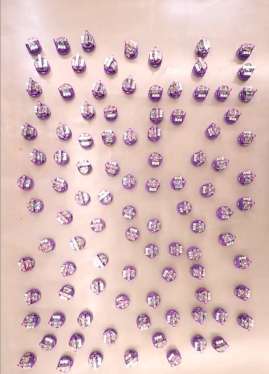
\includegraphics[width=0.16\textwidth]{coolfig/0.jpg}}\hfill
\subfloat[T = 20s]{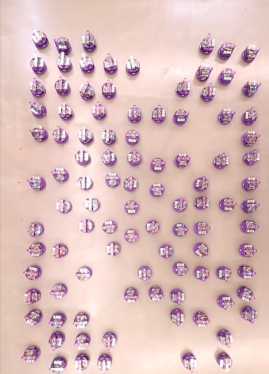
\includegraphics[width=0.16\textwidth]{coolfig/1.jpg}}\hfill
\subfloat[T = 64s]{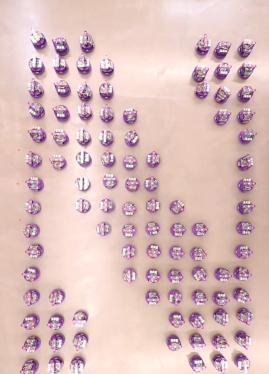
\includegraphics[width=0.16\textwidth]{IEEEtran/coolfig/2.jpg}}
\\
\vskip -10pt
\centering
\subfloat[T = 72s]{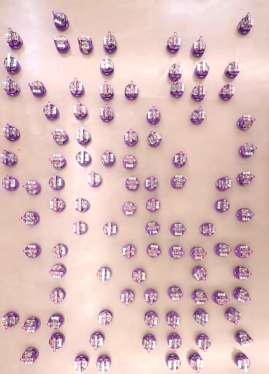
\includegraphics[width=0.16\textwidth]{coolfig/3.jpg}}\hfill
\subfloat[T = 80s]{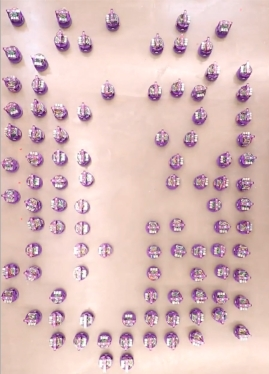
\includegraphics[width=0.16\textwidth]{coolfig/4.jpg}}\hfill
\subfloat[T = 112s]{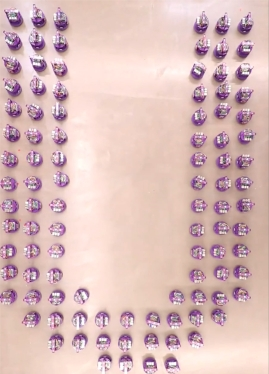
\includegraphics[width=0.16\textwidth]{coolfig/5.jpg}}

\caption{Still images from a 100 robot shape formation experiment.  The robots start in a random configuration, and move to form the desired ``N" shape.  Once this shape is formed, they then form the shape ``U".  The entire sequence is fully autonomous using the distributed algorithm described in this paper.}
\label{fig:frames1}
\end{figure}
\captionsetup[figure]{labelformat=default}



In general, the complete shape formation problem can be divided into two subproblems: assignment of robots' locations in shape, and formation control. 

The assignment subproblem tries to divide the goal locations among the individuals, often in an optimal way such as minimizing the total distance traveled by the swarm. This problem has been well studied and there are several algorithms which can find the optimal assignment, including the Hungarian algorithm  \cite{huang}, auction algorithms  \cite{a1, a2}, and iterative methods  \cite{i1, i2}. Recent work shows that some certain assignments which minimize a cost of interest can help to reduce the computational complexity of path planning problems. One typical cost of interest used is the sum of the distance traveled by all agents \cite{e1, capt, centralized}, and the other cost of interests are the sum of the square distance traveled \cite{goalassign} and the maximal distance traveled \cite{peter}, which help to minimize the total time elapsed. In these methods, the calculation for the assignment is handled by a centralized coordinator. These centralized strategies can deliver a solution to the assignment problem, but does not easily scale to large numbers of robots, presents a single point of failure, and does not easily adapt to situations where the number of robots is unknown or can vary.  

Unsurprisingly, the distributed assignment methods, on the other hand, can often scale well to the number of robots, and can be more robust to failures \cite{particle} and varying numbers of robots. Past efforts try to solve the distributed assignment problem by following an incremental distributed refinements process \cite{nanthan, e2}. Here, the order how agents explore each goal has significant effect on convergence rate. In \cite{nanthan}, the agents follow a pre-assigned order which assures that a correct assignment of agents to tasks is always achieved after exploring at
most a polynomial number of assignments.  In  \cite{e2}, authors obtained an efficient convergence by forcing agents to follow a certain path. This path is collision free when agents have infinitely small size, but when agents have finite size, the path cannot provide a collision free guarantee.

After determining the role in shape, each agent then needs to move cooperatively to form the desired shape. In the past, many methods to produce the formation have been proposed. According to the types of actively controlled variables \cite{survey} such as agent's position or distances to the neighbors, formation control methods can be categorized into local-measurement-based methods \cite{graphtext, distance, dis1, dis2, dis3, dis4, bearing, displacement, pos1, pos2, pos3, pos5, rhc}, and position-based methods \cite{e1, capt, centralized, goalassign, d1,d2,d3,timeopt, c1,c2,c3,global, orca, van2011reciprocal, alonso2018cooperative, bufferedvonori,rrt, swarmbarrier, p1,p2, p3, capt,pri,peter}. 


In local-measurement-based methods \cite{graphtext}, the agents form the desired shape by actively controlling its distance \cite{distance,dis1,dis2,dis3,dis4}, bearing \cite{bearing}, or both \cite{displacement,pos1,pos2,pos3,pos5}, relative to its neighbors. This type of methods only require the use of relative measurements therefore can be employed in the GPS-denied environments, e.g. indoor environments. For local-measurement-based methods, the challenge is how to obtain the global stabilization to the desired formation using only peer-to-peer information \cite{displacement}. 


Some methods achieve the global stabilization by relying on the leader agents \cite{dis4,pos2,pos3,pos5}. In these methods, the leader(s) tracks its desired trajectory, and the non-leader agents are tasked to maintain certain graph structures rooted from the leader agent(s) where each vertex characterized an agent and each edge characterizes an inter-agent measurements, such as  distance or relative position. These methods allow the swarm to stabilize to a formation that is even dynamically moving, but require an additional leader selection phase to assign a role (leader or non-leader) to each agent.



The methods proposed in \cite{displacement, pos1} are leaderless, these methods enable a group of
agents to reliably produce a rigid shape, using the relative positions of agent's neighbors. Nevertheless, in order to achieve global stability, the method proposed in \cite{pos1} needs the communication graph amongst agents to be complete, and the method proposed in \cite{displacement} requires the desired formation to satisfy some specific topological conditions.


While local-measurement-based methods permit operations in GPS-denied environments, they often requires a centralized coordinator, or the use of a complete communication network, to initially assign each robot a position in final shape. Moreover, without any additional mechanism, it often fails to provide an absolute collision avoidance guarantee when agents have finite size.



To the contrary, in position-based methods, the desired formation is achieved by
actively controlling the agents' positions. This type of methods require that each agent is able to measure their own positions with respect to a global coordinate system. Here, the challenge is how to efficiently generate collision-free trajectories where agents can achieve the desired formation by moving to goal locations. 


Some previous work tackled the problem in a discrete setting  \cite{d1,d2,d3,timeopt}, while others solved the problem in a continuous setting  \cite{c1,c2,c3,global}. As expected, these centralized methods suffer from the curse of dimensionality (because the dimension of swarm's joint configuration space increase exponentially over swarm size), hence often cannot easily scale to large-scale swarms, such as a swarm of over 1000 agents.

An alternative method is to use an artificial potential function to guide agents to the desired formations using gradient descent. Some authors make use of gradient descent to drive agents to goals \cite{p1,p2}, and some use the potential function to modify current trajectories locally to prevent collision and maintain connectivity  \cite{p3}. The drawbacks for this kind of method are that it may take a long time to converge, and there is no guarantee provided that they can form the desired shape \cite{capt,pri}.



Distributed multi-agent path planning is a well studied topic. Some methods are based on local measurements, either relative velocities \cite{orca, van2011reciprocal,, alonso2018cooperative}, or relative positions \cite{bufferedvonori}, but none of these methods can provide a deadlock free guarantee;  agents can get stuck in a situation where no action can be made for further progress, yet the shape is incomplete. In fact, in our review of distributed path planners \cite{orca, van2011reciprocal,bufferedvonori, swarmbarrier, rhc, alonso2018cooperative}, none of the methods can provide a deadlock free guarantee and absolute collision free guarantee at the same time. This is also suggested in \cite{bufferedvonori}, which also claims that no deadlock free distributed path planner that is with absolute collision free guarantee exists. Other approaches make use of the communication among agents, but in order to guarantee the correctness of the method, require either a lossless fully connected network \cite{rrt}, or precise velocity control \cite{capt}, which can be difficult to guarantee when implemented in a physical system. In \cite{swarmbarrier}, authors presented a distributed collision avoidance strategy which can resolve some certain types of deadlocks using local communication only, but the method cannot resolve all types of deadlocks. A distributed receding horizon control (RHC) based method is proposed in \cite{rhc}, this method requires only the use of relative sensing in robot's local coordinate frames, and is able to provide mathematical guarantees on the achievement of the rendezvous, however, it has not been shown that the method can provide collision free guarantee and absolute deadlock free guarantee at the same time.    

In this paper, we present a fully distributed shape formation algorithm where each agent is identically programmed and takes the same input, a set of goal points that describes the desired shape. Each agent will use local communication to actively refine the goal assignment and control its position in a distributed fashion. To the best of our knowledge, and supported by \cite{bufferedvonori}, our algorithm is the first provably correct fully distributed shape formation algorithm that can also provide absolute collision free and deadlock free guarantees, requiring only the use of local communication. Moreover, the physical experiments and simulations presented show that our algorithm is robust to real world non-idealities, such as communication errors, sensing errors, and imperfect robot motion.


\IEEEdisplaynontitleabstractindextext
\section{problem definition}
In this paper, we propose an algorithm that when given a set of desired target points (which are described by a set of nodes on a grid), moves a swarm of mobile agents so that each agent is located at a target position, and no target position has more than one agent. For each agent, the set of target positions are known a prior, moreover, all the agents agree on the same global reference frame. This algorithm must distribute the target positions among the agents and then drive the agents to their corresponding target position without collision. The system is distributed, agents are identically programmed, and act based on local information gathered through communication. In this section we will formally state the problem and introduce the notations used in paper. 

\subsection{Robot Model}

Agents are modeled as 2D omni-directional robots equipped with position and orientation sensing, i.e. each agent can measure its own position and orientation in a global coordinate system at all times. Each agent is treated as a circle with a finite radius $r$ and can move in any direction at two possible speeds: 0 or $v_m$. Additionally, each agent is able to communicate with any robot lying within its communication range $R\geq4\sqrt{2}r$. To simplify the analysis and description, we here assume that:

\begin{enumerate}[label=(\alph*), leftmargin=*]
    
     \item Each agent has the same clock frequency $f_{clock}$;
     \item Each agent is able to constantly transmit messages to the neighbors in communication range at a fixed rate $f_{comm}$;
     \item The local inter-agent communication is lossless;
   
    \item Each agent has the same $v_m$;
     \item The communication latency is negligible. 
\end{enumerate}

\noindent Note that here we do not have any assumption on the phase of the robot clock's relative to each other, they can be asynchronous in phase. When the algorithm is implemented in the real world, these assumptions can be relaxed to accommodate the real-world non-idealities, see section \ref{experi} for detailed discussion. 

\label{assumptions}


\subsection{Notations}
For the sake of describing our algorithm and formulating the problem, we introduce the notations as follows:

Let $A = \{a_1, a_2, ..., a_n\}$ be a set of agents, where each agent $a_i \in A$ has a position $p_{a_i}(t)\in {\mathbb{R}}^2$ at time $t$. For all $p\in \mathbb{R}^2$, $p^x, p^y$ denote $p$'s x and y components, respectively. $||\cdot||$ denotes the euclidean norm on ${\mathbb{R}}^2$ space and $\succ$ denotes the lexical order on $\mathbb{R}^2$ space, namely, $p_1\succ p_2$ if and only if: $p_1^x > p_2^2$, or $p_1^x=p_2^x$, $p_1^y>p_2^y$. Let $Q = \{q_1,..., q_m\}$ be a set of distinct target locations, where $q_i\in {\mathbb{R}}^2$, we assume that $\forall q_i, q_j \in Q, ||q_i - q_j|| \geq 2\sqrt{2}r$, i.e, in the desired shape no pair of robots collide with each other. Moreover, we use $T_{a_i}(t) \in Q$ to denote $a_i$'s assigned target position at time t. We assume that every agent has the same communication range $R$, and $N_{a_i}(t) \subset A$ denotes the set such that at time t, $\forall a_j \neq a_i$, $||p_{a_i}(t) - p_{a_j}(t)|| \leq R$ if and only if $a_j \in N_{a_i}(t)$, in the other words, $N_{a_i}(t)$ is the set of agents that are able to communicate with $a_i$ at time $t$.  

\subsection{The Problem Formulation}
Our task is to design an algorithm to move a swarm of $n$ identical robots, represented by set $A$, from their initial positions to an arbitrary connected target formation, represented by set $Q$. To simplify the problem, we assume $|Q|=|A|$. The algorithm should be deadlock free and collision free, that is:
\begin{itemize}

    \item $\exists t_{max} > 0$ such that at any time $t > t_{max}$, it holds that: $\forall a_i \in A$, $p_{ai}(t) = T_{a_i}(t)$, moreover, $\forall a_j \neq a_i, T_{a_j}(t) \neq T_{a_i}(t)$,
    \item  $\forall t\geq0$, for any two agents $a_i\neq a_j$, $||p_{a_i}(t) - p_{a_j}(t)|| \geq 2r$. 

\end{itemize}







\section{Approach}
To form the goal shape, each agent needs to pick a valid goal, and then move on a collision-free and deadlock-free path towards that goal without any centralized coordination. For this task, two subproblems arise. One of them is solving duplicated assignments, which is caused by the limited sensing ability of the agents. Agents don't have access to global information so they have to determine their targets based only on local information. This makes it possible that there exist multiple robots holding the same target. The other subproblem is planning each robot's motion based on local information so as to generate collision-free and deadlock-free paths toward the goals.  Additionally, if every agent's target is unique, the motion planner should guarantee that each agent will reach the target in a finite amount of time. 

In our method, the task is handled by two modules: the \textit{new goal selector}, which is used to pick a valid goal, and the \textit{motion planner}, which is used to plan the agent's motion. Each agent uses the \textit{motion planner} to move to its current goal, and if it encounters another agent holding the same goal, it uses the \textit{new goal selector} to pick another goal. A detailed description is shown as alg. \ref{al1}. Note that this algorithm runs on each agent of the swarm.

\begin{algorithm}[t]
\caption{General Framework for Shape Formation}
\DontPrintSemicolon
\label{al1}
%\SetAlgoLined
\small
\KwIn{ $Q=\{q_1, q_2, ..., q_m\}$ }
$T_{a_i}(t) \gets $ random element in $Q$\;
\While{True}{
 \If{$\exists a_j \in N_{a_i}(t)$, s.t. $T_{a_j}(t) = T_{a_i}(t)$}
     {run \textit{new goal selector} \textit{(alg. \ref{mh} Line 3-10)}\;}

 run \textit{motion planner} \textit{(alg. \ref{alg:main} Line 25-29)}\;
 }
\end{algorithm}




\subsection{Motion planning}

To generate a collision-free path, we first convert the continuous environment into a discrete grid, as shown in Fig. \ref{fig:grid}. Note that the grid here is the same grid goal points are located on.  Let $l$ be the length of the grid edge, where the constraint that $2\sqrt{2}r\leq l \leq \frac{R}{2}$ is enforced for the purpose of collision avoidance. Furthermore, we assume that there are no obstacles located in the environment. With this representation, each agent's path is given by a sequence of the waypoints, i.e. the nodes of the grids.

\begin{figure}[h]
    \centering
    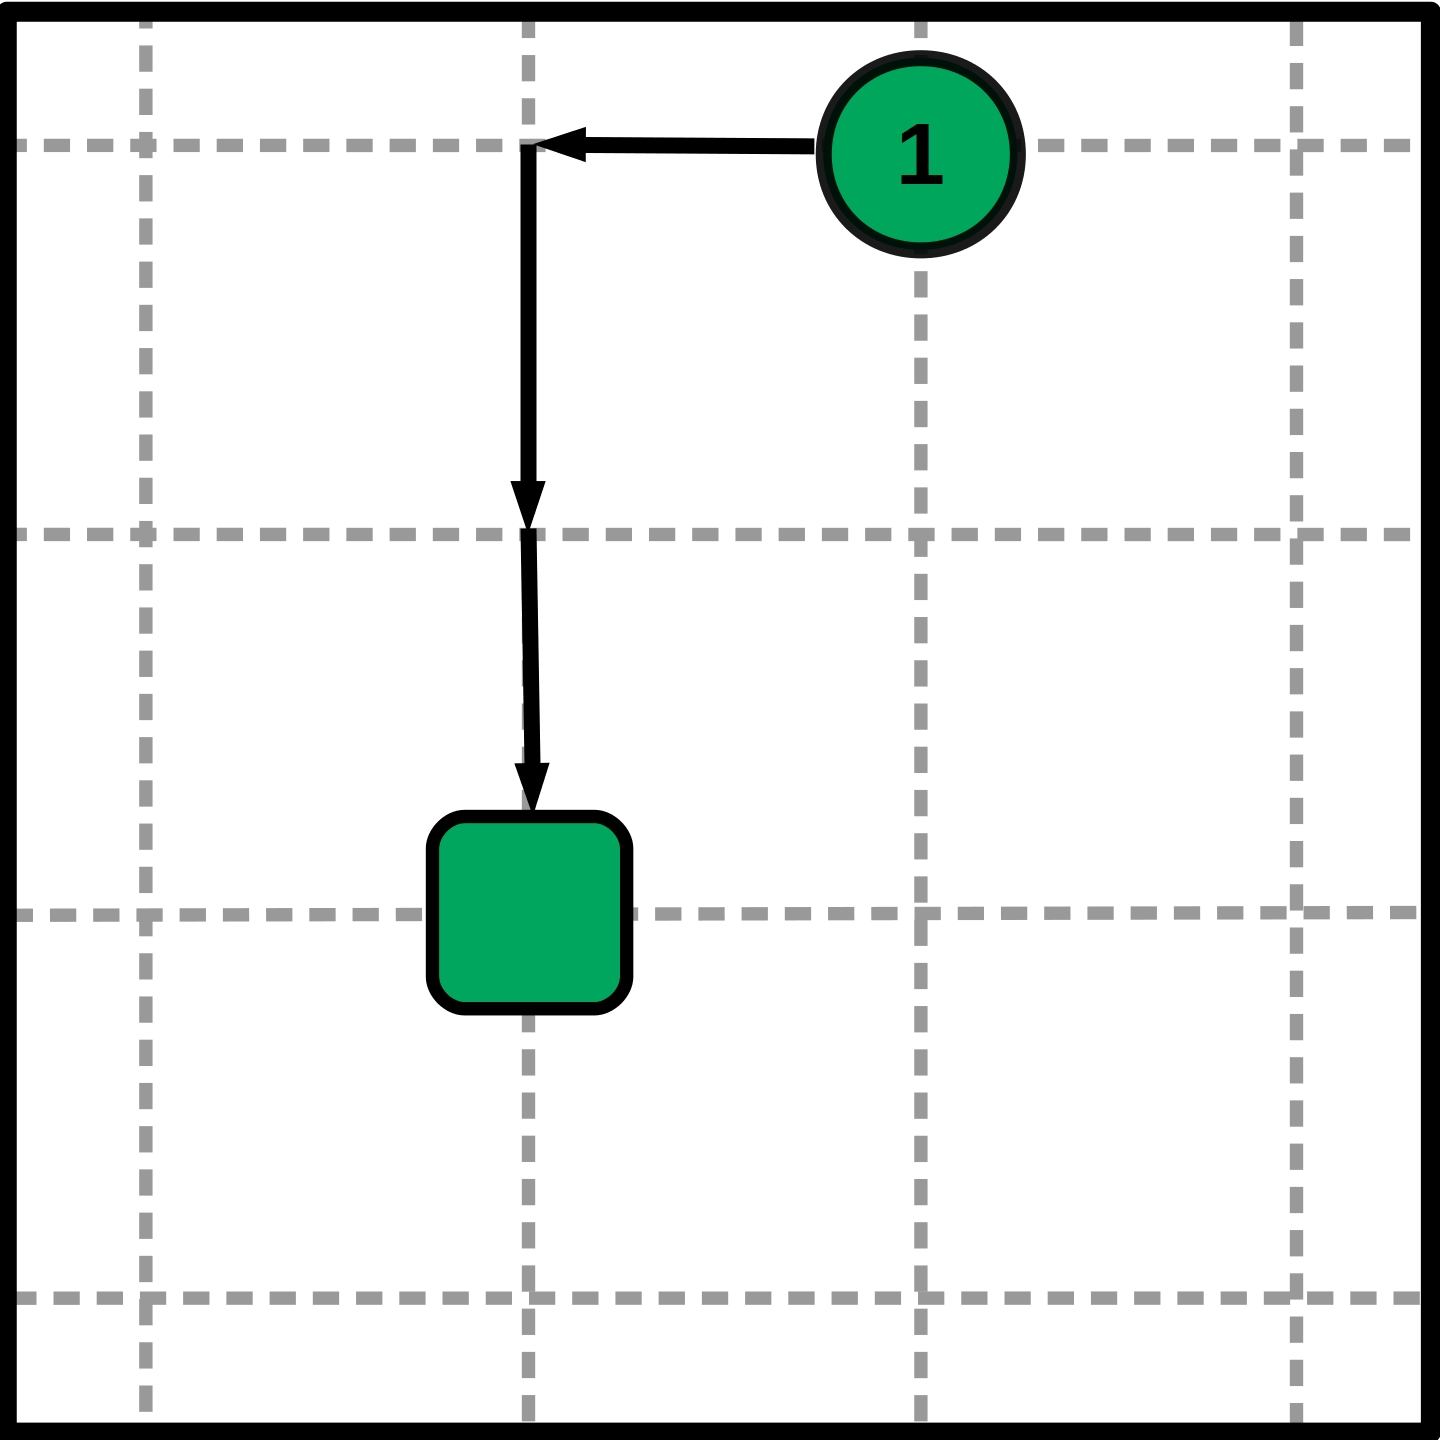
\includegraphics[width=0.15\textwidth]{traffic1/00.jpg}
    \hfill
    \includegraphics[width=0.15\textwidth]{traffic1/01.jpg}
    \hfill
    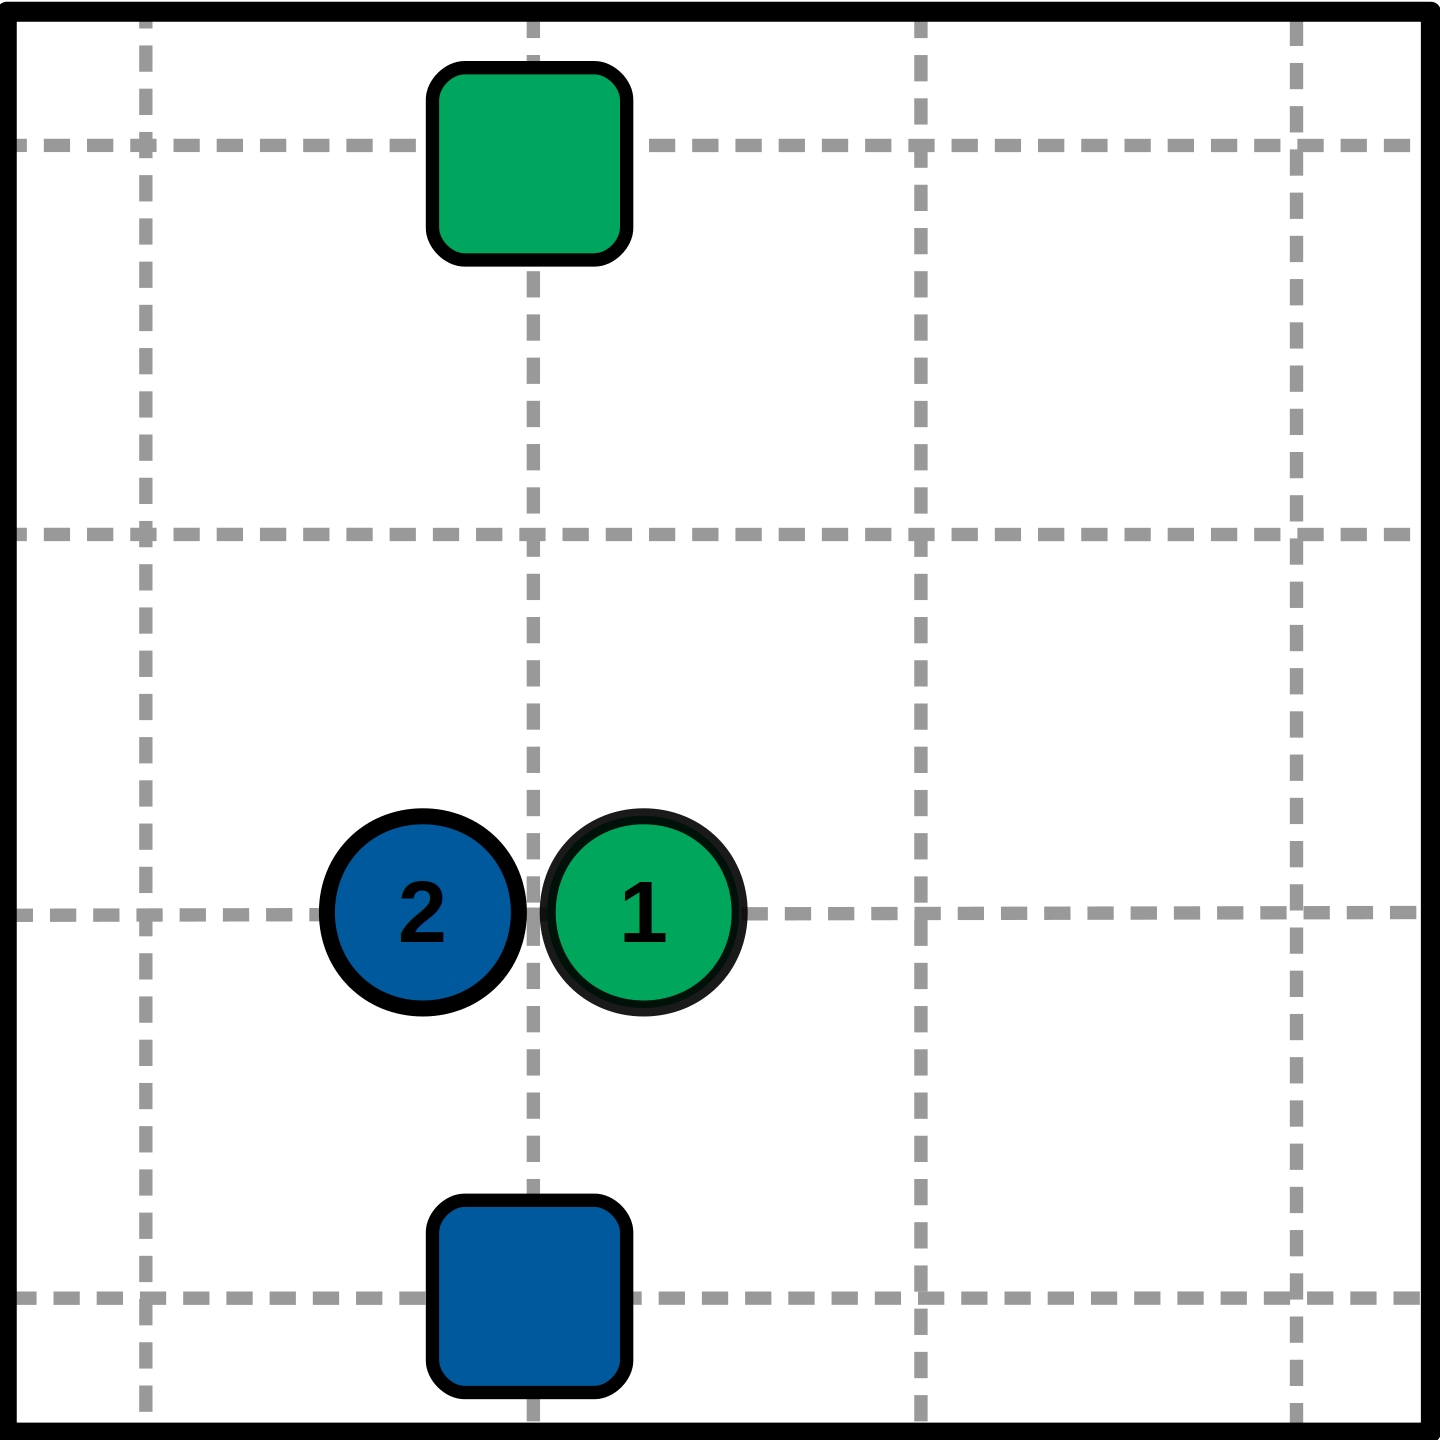
\includegraphics[width=0.15\textwidth]{traffic1/02.jpg}
    \caption{Illustration of the grid discretization of space and possible collision cases. The intersections of grey dashed lines represent the feasible waypoints, and agents travel on the edges between waypoints.  Each agent's position is shown with a colored circle and its goal point is shown with a square of the same color. Moreover, we label each agent with a unique number and use the arrow to show agent's incentive for next step. \textbf{(\textit{left})} a valid trajectory for a single agent to move to its goal.  The trajectory is shown as a sequence of arrows.  \textbf{(\textit{middle})} an edge collision, where blue and green robots both intend to travel on the edge in black, in opposite directions.  Here neither can make progress without collision.  \textbf{(\textit{right})} collision happens on a waypoint, where the blue and green robots try to move to the same waypoint at the same time, physically colliding.}
    \label{fig:grid}
\end{figure}


For every two adjacent waypoints, the motion controller enforces that the robots travel on the line segment between them. The motion controller plans every robot's motion, such that the following constrains are satisfied:



\begin{constrain} At any time t, no agent moves to the waypoint that is currently occupied by the other, and no pair of agents move towards the same waypoint at the same time.\label{cmp1}\end{constrain}

\begin{constrain} At any time t, no pair of agents travel on the same edge in opposite directions.\label{cmp2}
\end{constrain} 


For each agent located at any waypoint, there are five possible actions: move $north$, $east$, $south$, $west$, and $wait$. Agents should choose the action that greedily reduces the Manhattan distance to its goal point. Once the agent determines its next action, and if this action is not $wait$, it first uses communication to check whether the waypoint is occupied by any other agent. If it is occupied, the agent executes $wait$ and continues using communication to check the availability of the waypoint \textit{(alg. \ref{alg:main} Line 26-27)}. If there is no other agent occupying this waypoint, the agent then starts to check if any other agent wants to move to the same waypoint as it does. If there are multiple robots intending to go to the same waypoint $(x, y)$ at the same time $t$, then the robot $a_i$ whose current position $p_{ai}(t)$ is the lexically largest will go first \textit{(alg. \ref{alg:main} Line 28-29)}. 

As the agent moves towards its goal, it continually tries to improve its goal assignment, changing its goal based on local information.  When it senses a neighbor with whom a swapped goal would result in a reduced  pairwise traveled distance (in terms of Manhattan distance), it swaps goals with that neighbor \textit{(alg. \ref{mh} Line 11-15)}. If swapping goals with a neighbor does not change the pairwise distance traveled, they swap goals with a probability of 0.1 \textit{(alg. \ref{mh} Line 16-21)}.  When a goal conflict is sensed, i.e. a neighbor is seen that is holding the same goal point, one of the agents picks a new goal from $Q$ to eliminate the duplicated goal \textit{(alg. \ref{mh} Line 3-10)}. An illustration of the cases in which an agent may change its goal are shown in Fig. \ref{fig:i3}.  

It is possible that multiple agents (more than two agents) intend to swap the goals at the same time, for example, at time $t$, $a_i$ intends to swap the goal with $a_j$ while $a_j$ intends to swap the goal with the third agent $a_k$. In our implementation, the pairwise goal swap is achieved by 2-way handshake \textit{(alg. \ref{mh} Line 12, 18)}. Only the pair of agents who successfully handshake with each other can swap the goal. To be specific, when agent $a_i$ intends to swap the goal with $a_j$, if $p_{a_j}(t)\succ p_{a_i}(t)$, then it will take the role of \textit{client} in this handshake, otherwise if $p_{a_i}(t)\succ p_{a_j}(t)$, $a_i$ will act as \textit{server} in the handshake. A \textit{client} agent $a_i$ will send a handshake request to its intended goal swap peer $a_j$, which is a handshake \textit{server} since $p_{a_j}(t)\succ p_{a_i}(t)$, and then wait for the acknowledgement (ACK) from this \textit{server} agent $a_j$ for certain amount of time. On the other hand, a \textit{server} agent $a_j$ will wait for the handshake request from its intended goal swap peer $a_i$ for certain amount of time, which is a \textit{client} agent since $p_{a_j}(t)\succ p_{a_i}(t)$, and send back an ACK to $a_i$ after receiving the handshake request from $a_i$. Note that it is possible that a \textit{server} agent $a_j$ receives the handshake requests from other agents that is not its intended goal swap peer. When this happens, it will answer the requests from these agents with a negative acknowledgement (NACK) (or does not answer these requests at all so as to trigger the handshake timeout). The \textit{client} agent $a_i$ will update its goal only after receiving the ACK from the intended goal peer $a_j$, and the \textit{server} agent $a_j$ will update its goal after receiving the handshake request from its intended goal swap peer $a_i$.

\begin{figure}[h]
\centering
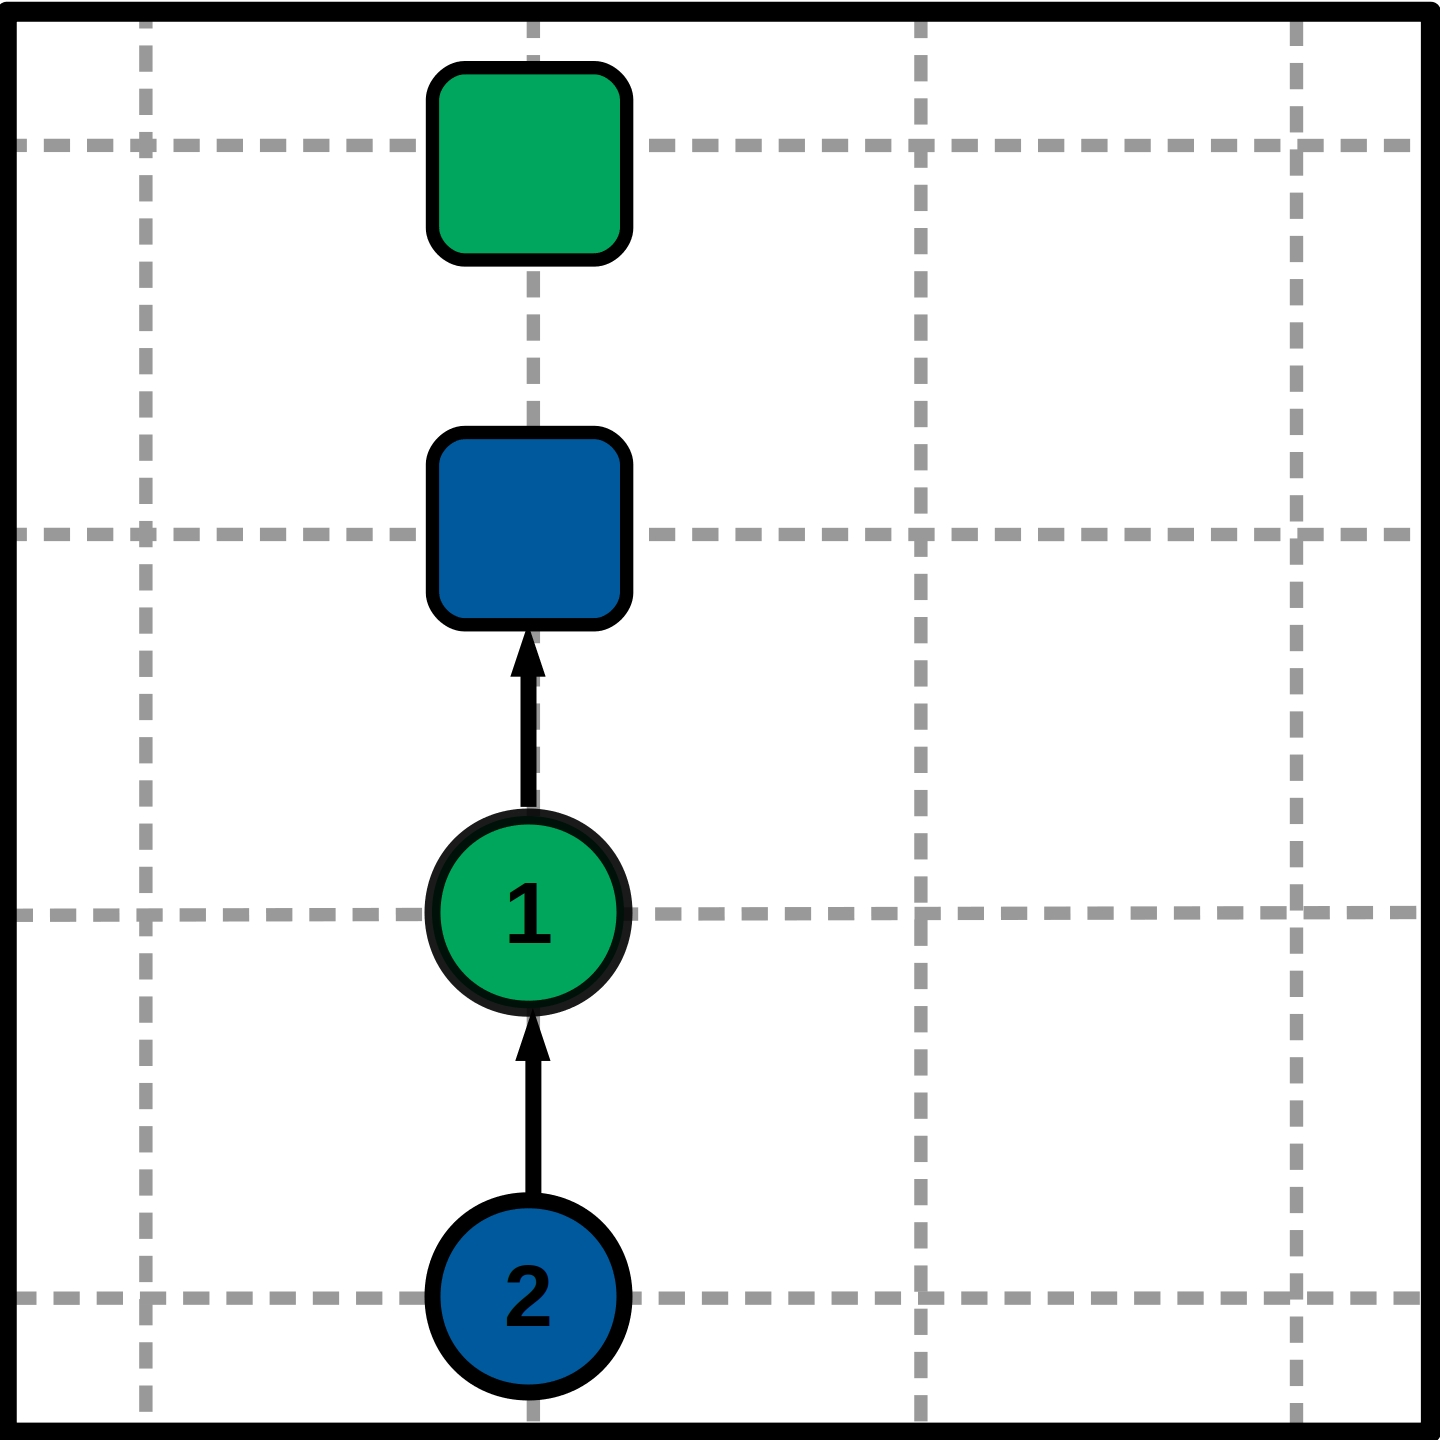
\includegraphics[width=0.15\textwidth]{traffic2/00.jpg}
\hfill
\includegraphics[width=0.15\textwidth]{traffic2/01.jpg}
\hfill
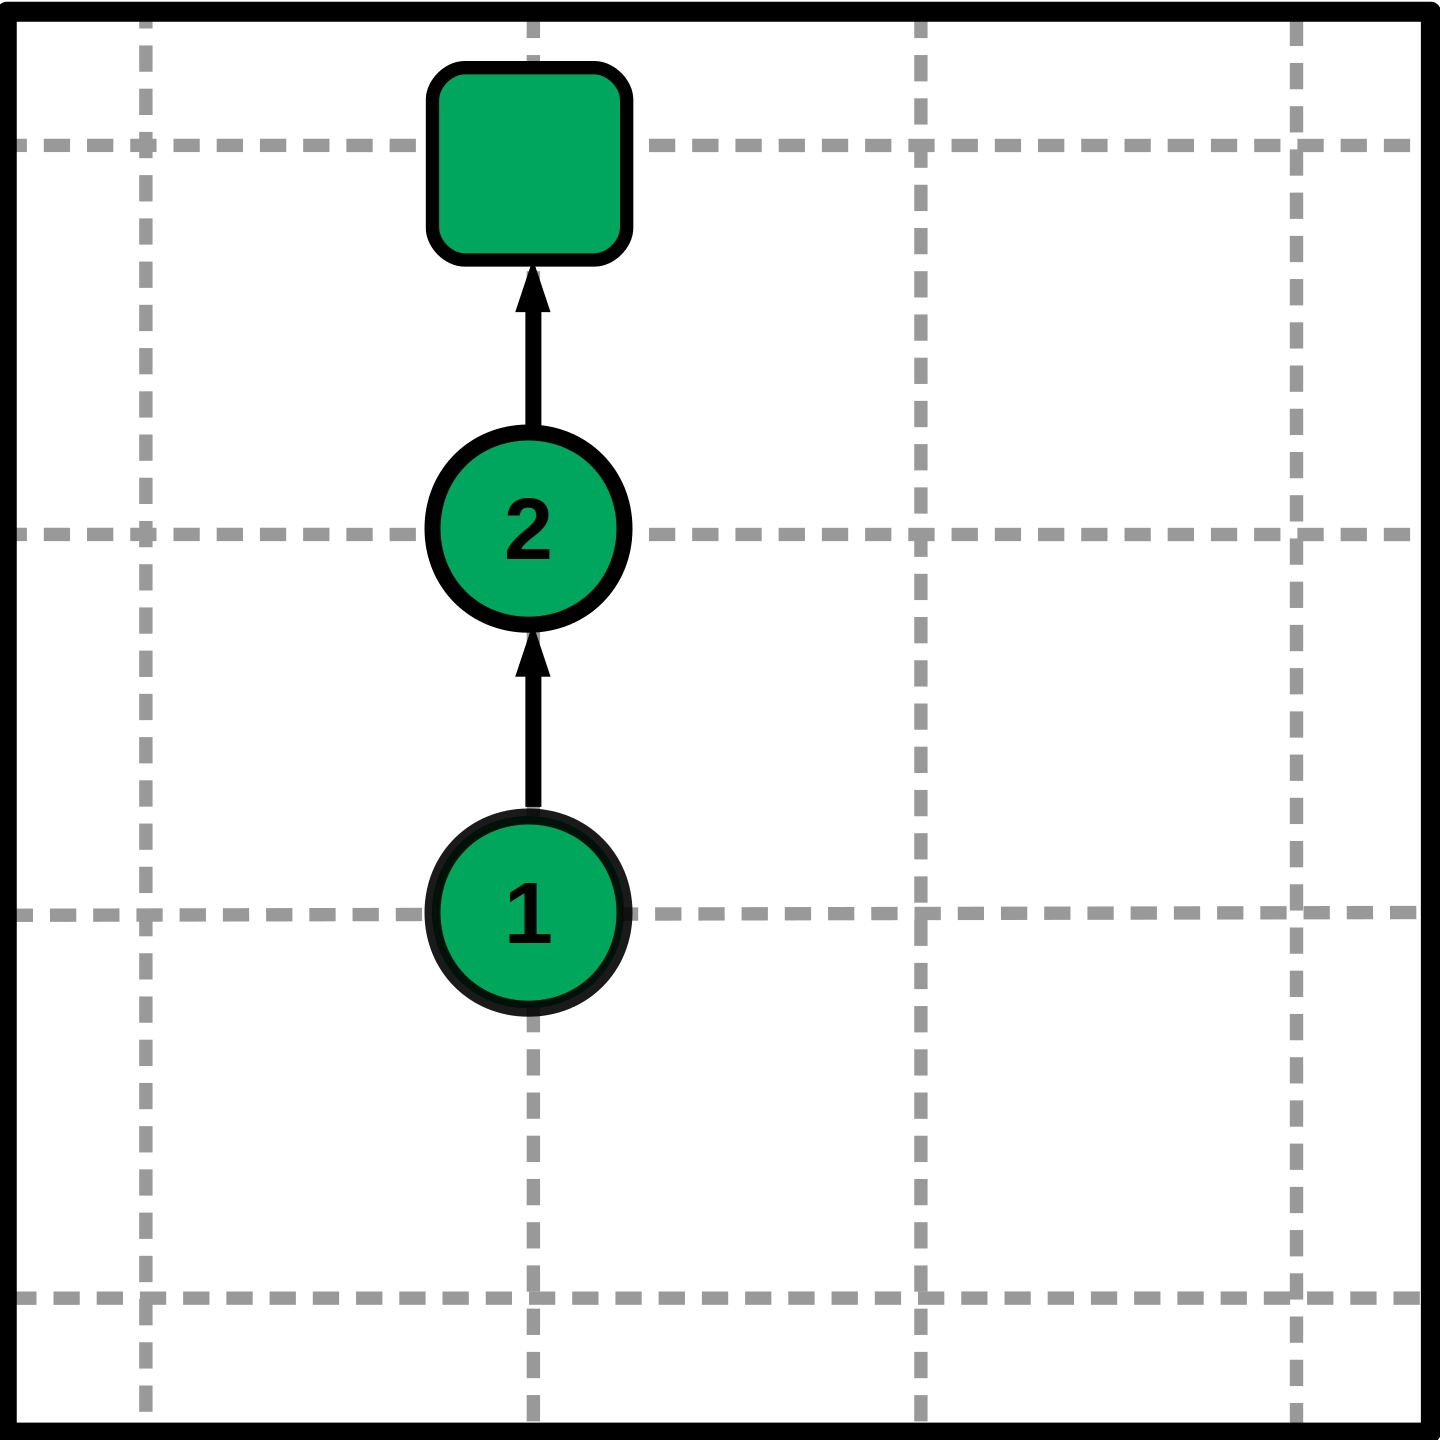
\includegraphics[width=0.15\textwidth]{traffic2/02.jpg}
\caption{Illustration of possibles cases where an agent may change its goal. All the information is encoded in the same way as Fig. \ref{fig:grid}.  \textbf{(\textit{middle})} For any pair of agents located within each other's communication range, if goal swap can help them to reduce the pairwise total distance traveled (in term of Manhattan distance), then goal swap occurs.  \textbf{(\textit{left})} If the goal swap doesn't affect the total pairwise travel distance, these two agents randomly decide whether to swap. \textbf{(\textit{right})} If both agents hold the same goal, one of them will run the \textit{new goal selector} algorithm to select a new goal from $Q$. }
\label{fig:i3}
\end{figure}
\label{motion planning}




\subsection{New goal selecting}
As we want each agent to have a unique goal in the end, the algorithm needs to eliminate any duplications in the assigned goals. For the \textit{new goal selector} algorithm, we desire the swarm to have as many different goals assigned as possible.  When the total number of assigned goals is equal to the size of the swarm, no pair of agents will have the same goal. This implies that the \textit{new goal selector} should keep the number of assigned goals growing.  Therefore, every time a new goal is selected, the total number of assigned goal points should be non-decreasing. 

\subsubsection{Random selector}
A simple \textit{new goal selector} would be a random selector. For every pair of agents $a_i, a_j$ that detect that they hold the same goal, if $p_{a_j}(t)\succ p_{a_i}(t)$,  where $\succ$ denotes the lexical order on $\mathbb{R}^2$ space, then $a_i$ randomly picks a new goal from the set $Q$. 

While the random selector can guarantee the process to be almost surely convergent, the probability of picking an  unassigned  goal will decay over the number of assigned goals, leading to a relatively long convergence time. We therefore introduce a heuristic to speed convergence.

\subsubsection{Gradient based selector}

The gradient algorithm, which is a well-known collective behavior, also known as hop-count algorithm \cite{mike,mike2},
 can be adapted to improve goal selection. It is a simple algorithm that involves two agent roles, the common agent and the anchoring agent, and both roles transmit a single message containing an position $q_u$ and a hop-count $h$. Each common agent listens to messages from its neighbors in communication range $R$, finds the message with the lowest hop-count received, $(q_u^x,q_u^y,hop)$, and then transmits the message $(q_u^x,q_u^y,hop+1)$ \textit{(alg. \ref{alg:main} \textit{Line 17-19})}.
 
The basic hop-count algorithm from  \cite{mike, mike2} can be modified in the following way to allow for better goal selection. An agent will take on the anchoring role when it is one grid length away from an unassigned goal point $(q_u^x,q_u^y)$ (by `` unassigned  goal" we mean the goal that is not assigned to any of the agent's neighbors in communication range), and transmit the message $(q_u^x,q_u^y,0)$ \textit{(alg. \ref{alg:main} \textit{Line 20-24})}. An anchoring agent will become a common agent when it no longer detects a  unassigned  goal that is one grid length away. Every agent $a_i$ keeps the latest goal point $(q_u^x, q_u^y)$ it transmits as the candidate goal $q_u$. When $a_i$ detects that there is other agent $a_j$ holding the same goal and  $p_{a_j}(t)\succ p_{a_i}(t)$, it then uses the current candidate goal $q_u$ to update its goal $T_{a_i}(t)$ (alg. \ref{mh} \textit{Line 3-10}).

\begin{figure}[t]
\centering
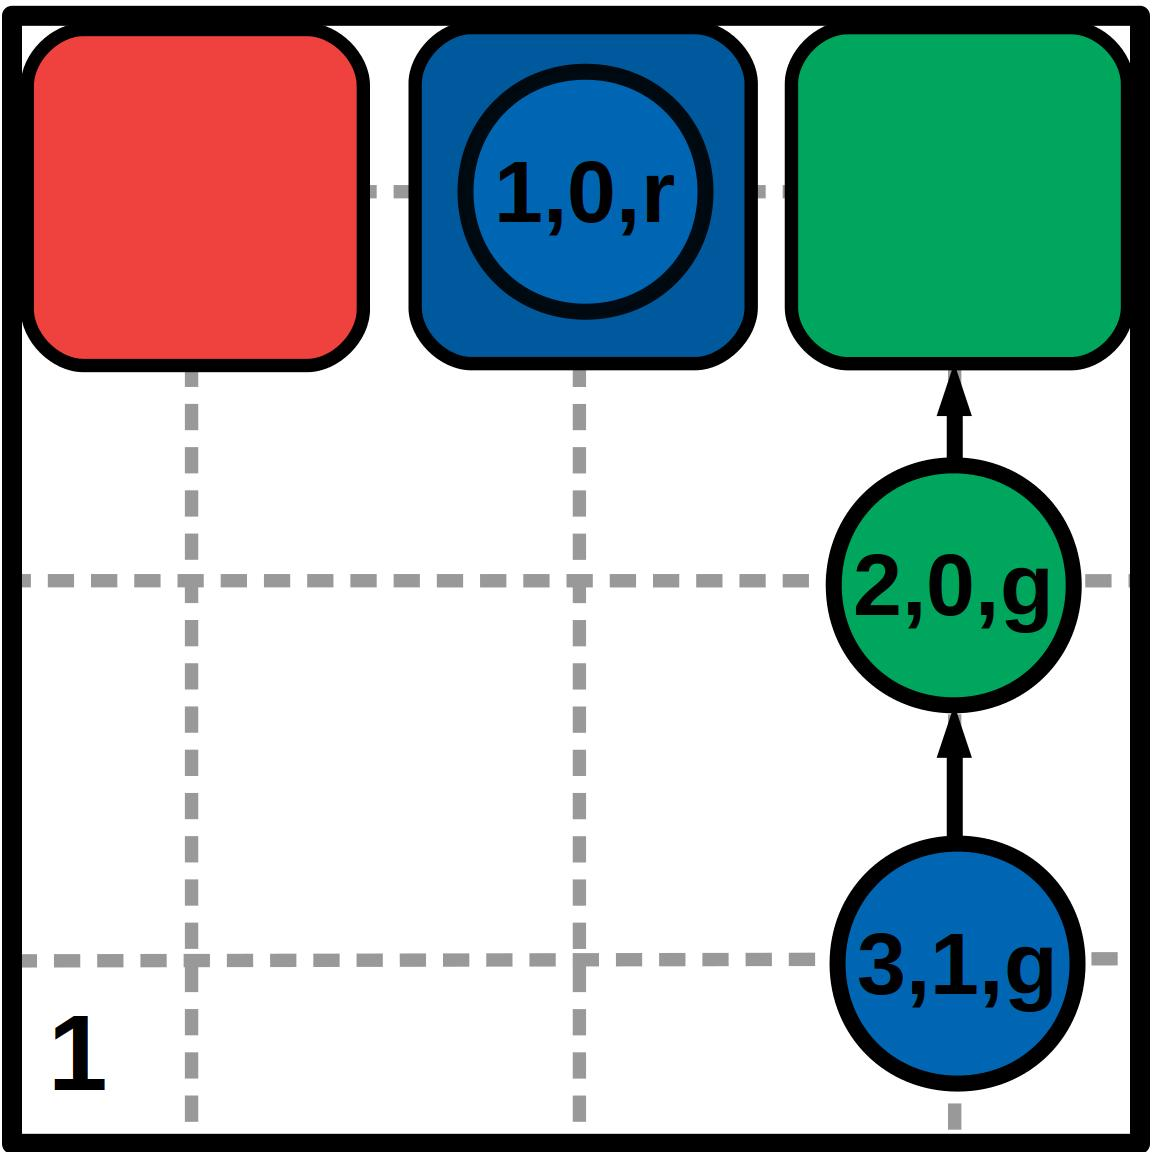
\includegraphics[width=0.115\textwidth]{IEEEtran/hopcount/1.jpg}
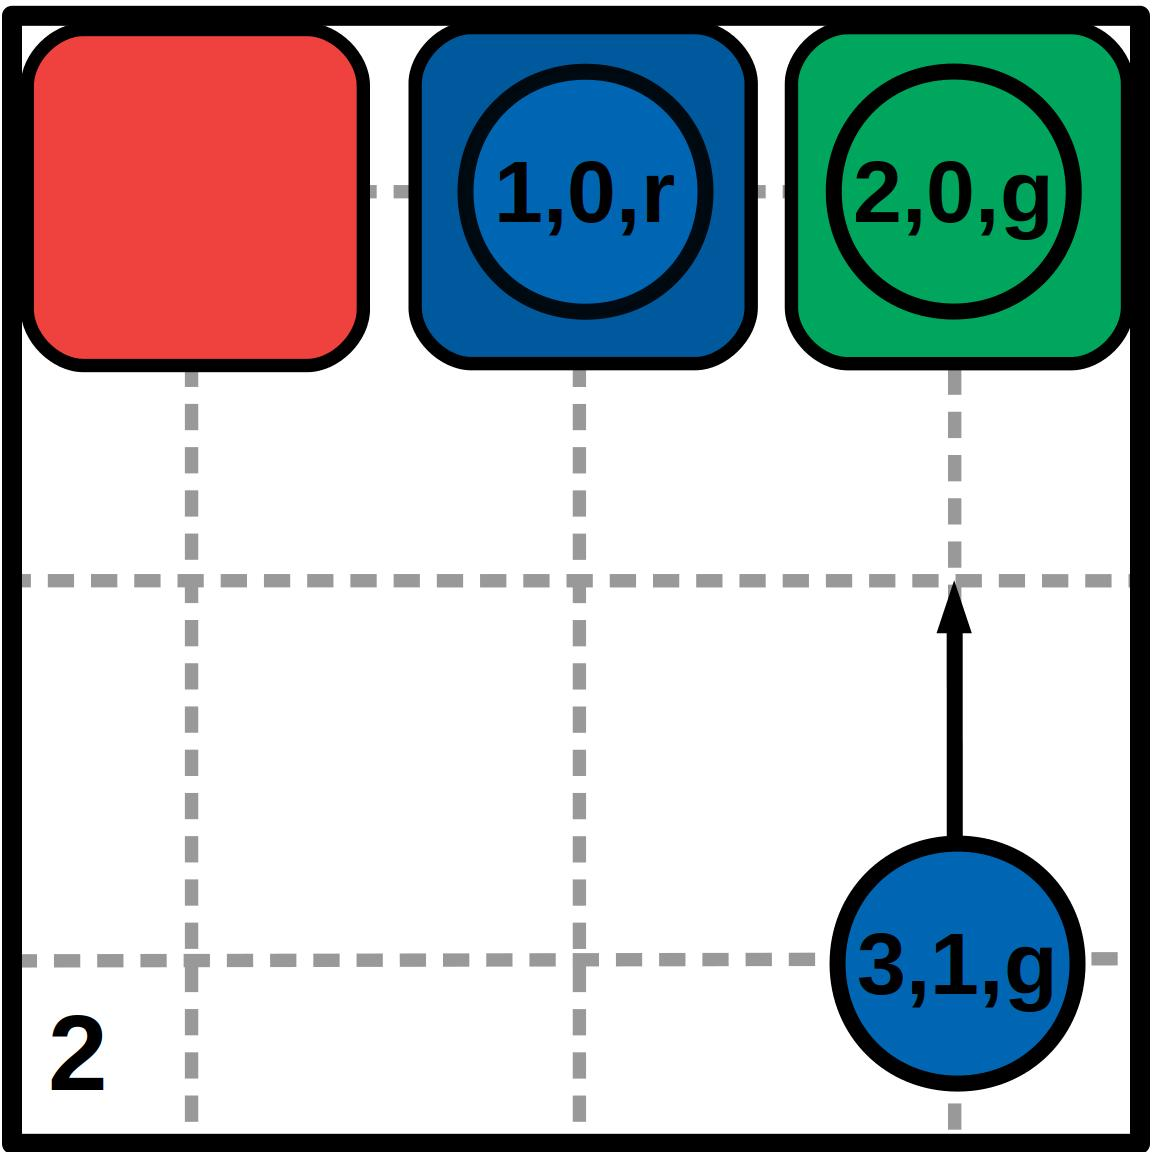
\includegraphics[width=0.115\textwidth]{IEEEtran/hopcount/2.jpg}
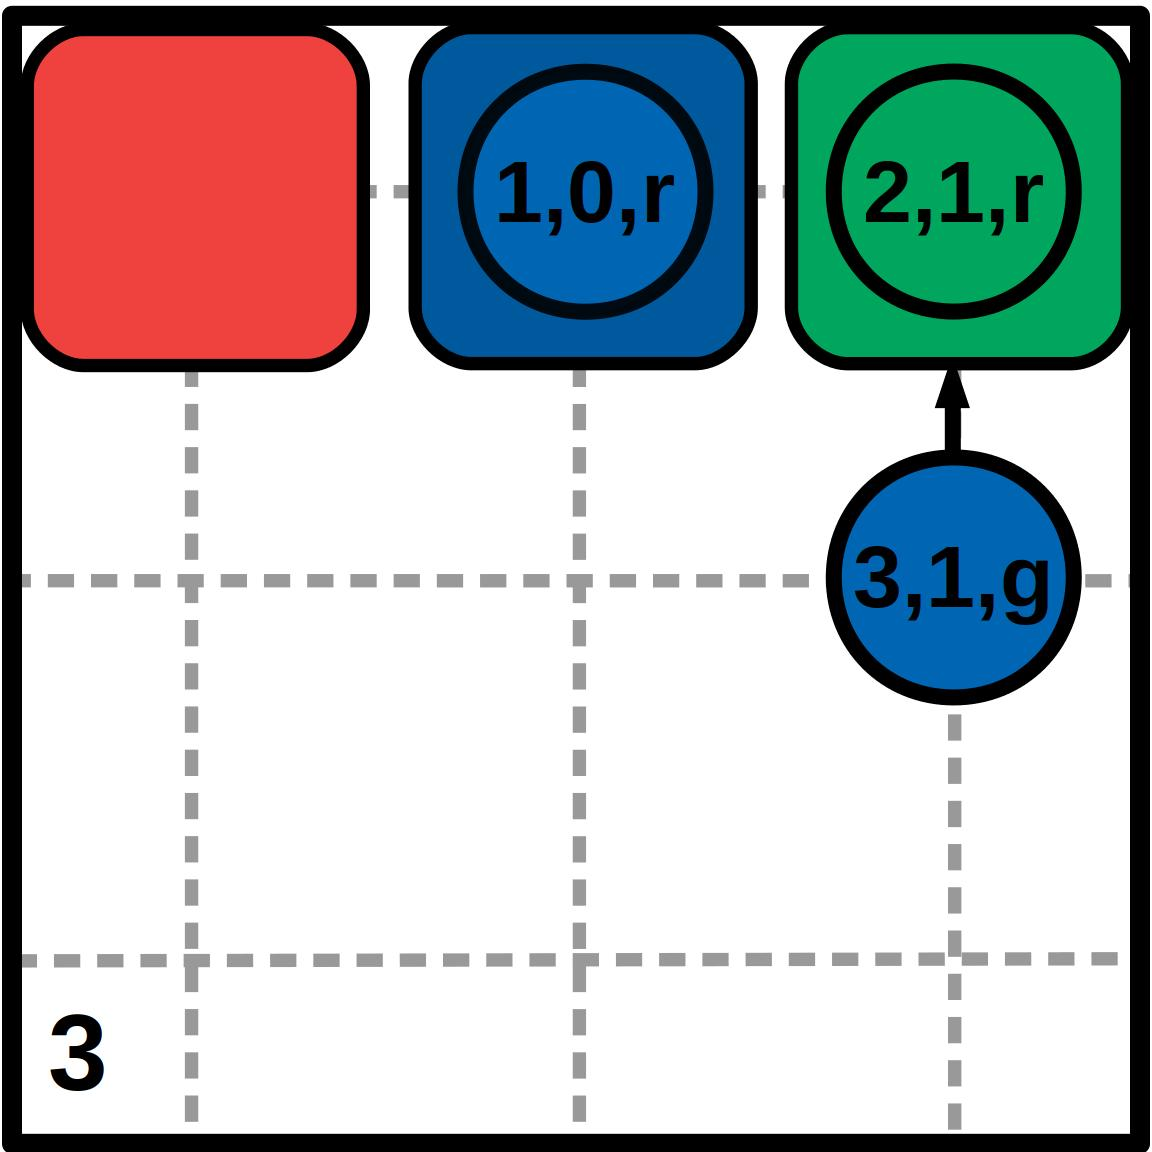
\includegraphics[width=0.115\textwidth]{IEEEtran/hopcount/3.jpg}
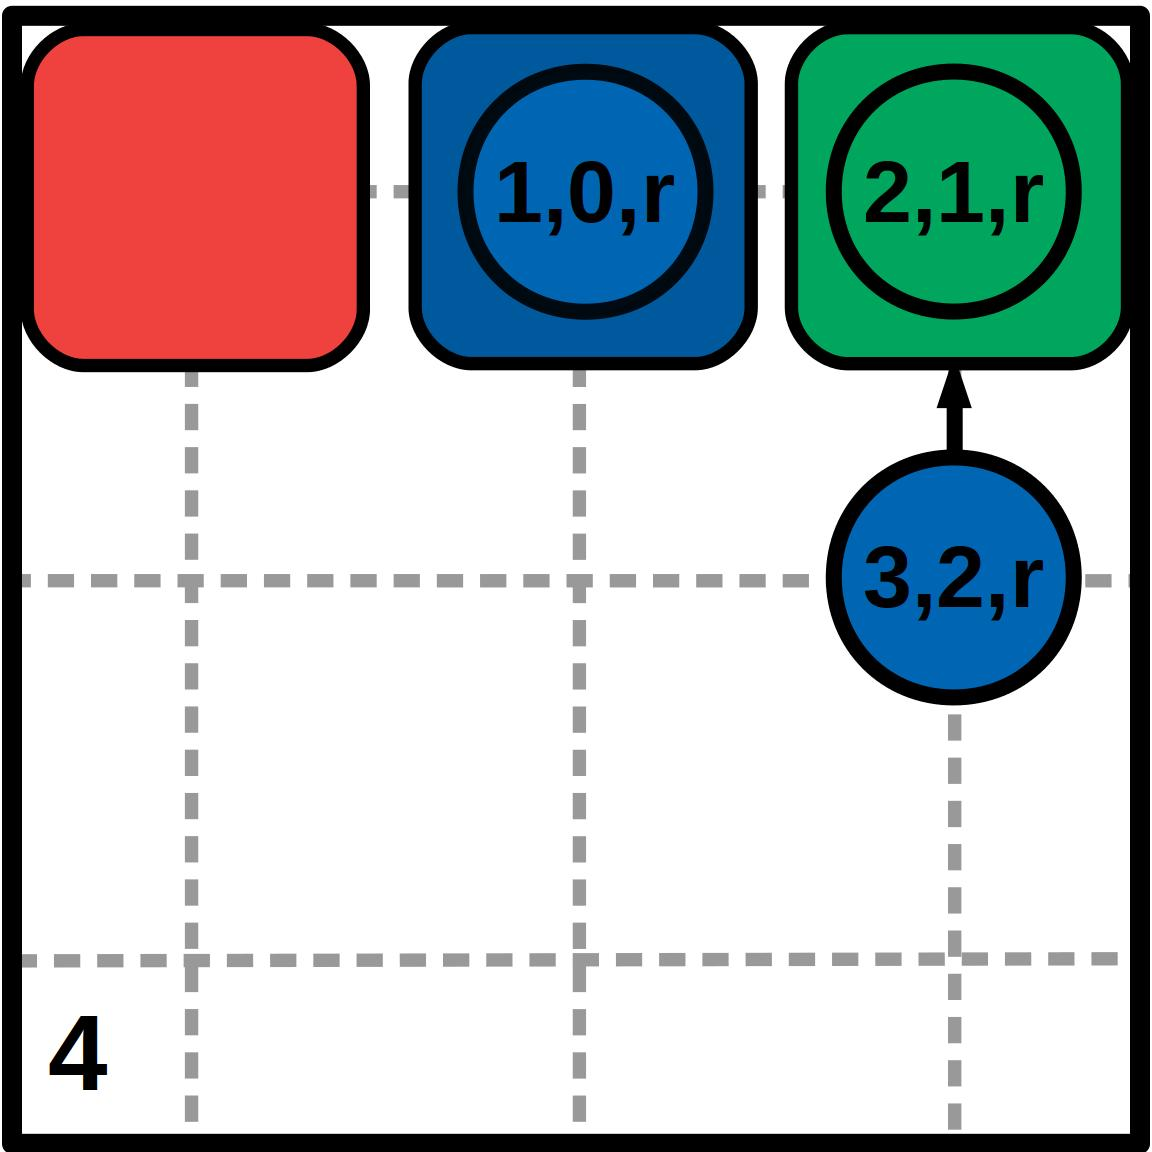
\includegraphics[width=0.115\textwidth]{IEEEtran/hopcount/4.jpg}

\caption{An example of agents using gradient based selector to update their goals. Goal positions are shown as a colored square, agent positions are shown as a circle who's color matches its current goal. Agents are labeled with its index $i$, hop count value $hop$, and candidate goal $q_u$ color (r-red, b-blue, g-green) respectively. For this example, we assume that each agent's communication range is one grid length. Initially, in \textbf{frame1}, agent $a_1$'s goal is blue, $a_2$'s goal $T_{a_2}$ is green and $a_3$'s goal $T_{a_3}$ is blue. In \textbf{frame 2} agent $s$ and $s$ move towards their goal, with $s$ arriving at its goal.  In \textbf{frame 3} the hop count is updated.  In \textbf{frame 4} agent $s$ sees $s$ with the same goal, and since $s \succ s$ changes goals, choosing the goal indicated by the hopcount message.}
\label{fig:hop}
\end{figure}




This gradient based selector helps to prevent an agent from selecting a goal that is already occupied, while also propagating information about valid goals throughout the entire swarm.  This helps increase the possibility that the new goal generated from ``new goal selector" is valid, i.e. the goal has not been occupied by other agents yet. See Fig. \ref{fig:hop} for a graphical illustration.


In addition, the swarm can also use the gradient hop count to detect whether the shape is completed. If the shape is completely formed, there will be no anchor nodes in the swarm, so the gradient value of each agent will increase temporally.  If any agent holds a gradient value larger than the number of agents, then the agent knows there are no anchor nodes, and therefore the shape is completed. Once any agent detects that the shape is complete, it will send a message which propagates across the entire swarm telling every other agent that the shape is complete. 


\subsection{Implementation}
\label{implementaion}
In this section, we describe the implementation of shape formation algorithm using gradient based selector in detail. The algorithm consists of three components: main
component, broadcast component, and goal manager. The main component coordinates agent's motion based on the information coming from its neighbors in communication range so as to avoid collision; the broadcast
component constantly transmits messages to neighbors at a fixed frequency $f_{comm}$, and the neighbors in communication range will use these information to coordinate their traffic; the goal manager refines agent's assigned goal so as to eliminate the duplicated assignment and resolve the deadlocks. These three components can be implemented using three separate threads running on each agent that communicate through shared memory. The sketches of these three modules are shown in alg. \ref{alg:main}, \ref{com module}, and \ref{mh}. Note that all the variables are thread-public.

\begin{algorithm}[h!]
\caption{Main Component}
\DontPrintSemicolon
\label{alg:main}
\small
\KwIn{$Q=\{q_1, q_2, ..., q_m\}$}
\SetKwBlock{empty}{}{}
$wp\gets$ current waypoint\;
\small
$hop\gets \infty$\;
$q_u\gets$ random element in $Q$ \;
$T \gets $ random element in $Q$\;
\textit{next\_step} $\gets$ current waypoint\;
$\Delta t\gets\frac{2}{f_{comm}}$\;
\textit{last\_check} $\gets$ \textit{clock()}\;
\While{True}
{
     
    \textit{surroundings}$\gets${\footnotesize
    \{$(wp^x-l, wp^y), (wp^x, wp^y-l), (wp^x+l, wp^y), (wp^x, wp^y+l)$\}}{\scriptsize\tcc*[r]{ the set of waypoints one grid length away from current waypoint.}} 
    \textit{wait\_flag} $\gets 0$ \;
  \For({\scriptsize\tcc*[f]{find the next waypoint}})
 {\small i in surroundings} 
 {\small \If{ choice of i reduces distance to goal}{
    \textit{next\_step }$ \gets$ i\;  
    \textbf{Break}\;   
   }
  }
  \small
  \textit{msg\_buff}$\gets$ all messages received since \textit{clock()} - $\Delta t$\;
  \If {msg\_buff is \textbf{not} empty}{
  \scriptsize{\tcc*[h]{find the message that contains the lowest hop count value.}}\;
  \small
  \textit{msg\_min} $\gets $ the message in \textit{msg\_buff} that contains the lowest \textit{message.hop}\;
 $hop\gets$1 + \textit{msg\_min}.\textit{hop}\;
 $q_u\gets$\textit{msg\_min}.$q_u$\;
 \For({\scriptsize\tcc*[f]{check if there is any  unassigned  goal one grid length away}}){\small i in surroundings}
 {\small 
  \If{\footnotesize $i\in Q$  \textbf{and} $\forall$ msg$_j$ in msg\_buff, msg$_j$.$T\neq i$}{ 
   $q_u\gets i$\;
   $hop\gets 0 $\;
   \textbf{Break}\;
   }
   }
 \small  
  \For({\scriptsize\tcc*[f]{loop through all the messages in msg\_buff to check if there is any potential collision}}){\small i in msg\_buff}{\small 
    \If{i.wp == \textit{next\_step}}
        {\textit{wait\_flag} $\gets 1$ \scriptsize{\tcc*[f]{next\_step is occupied}}\;  
    }
    \If{i.next\_step == next\_step \textbf{and} i.$p \succ p$}
    {\textit{wait\_flag} $\gets 1$\scriptsize{\tcc*[f]{other agent with higher priority intends to go to the same waypoint}}\;
    }
    }
    }
    \If(\scriptsize{\tcc*[f]{there is no potential collision and the agent has stay at the current waypoint long enough}}){\small wait\_flag == 0 \textbf{and} clock() - last\_check $> \Delta t$ }
    {\small
    $wp\gets$\textit{next\_step}\;
    
    agent moves to $wp$\;
    \textit{last\_check} $\gets$ \textit{clock()}\;
  }
  \small
  \Else{stay at current waypoint}
  
}
\end{algorithm}

\begin{algorithm}[h!]
\caption{Broadcast Component}
\DontPrintSemicolon
\label{com module}
\small
\While{True}
{

\scriptsize{\tcc*[l]{Forge the message to be transmitted, the message contains: agent's current position, current waypoint, next waypoint, current goal, candidate goal, and hop count value.}}
\small
\textit{msg}$\gets$\textit{\{$p$, $wp$, next\_step, $T$, $q_u$, $hop$\}}\;
 transmit \textit{msg} \;
 sleep $\frac{1}{f_{comm}}$\;
 }
\end{algorithm}

\begin{algorithm}[h!]
\caption{Goal Manager}
\DontPrintSemicolon
\label{mh}
\small
\While{True}
{
\scriptsize{\tcc*[l]{We use $a_i$ to denote the agent that is executing this thread}}
\small
 \If {receive a msg\_in from any other agent $a_j$}{
 \If{$a_j$ holds the same goal}{
   \If{$p_{a_j}\succ p_{a_i}$}{
   \If{rand(0, 1.0) $>$ 0.1}{
   $T \gets q_u$\;
       \textit{last\_check} $\gets$ \textit{clock()}\scriptsize{\tcc*[l]{The goal changes, as a result, \textit{alg. \ref{alg:main} Line 11-13} may change \textit{next\_step}, hence we need to reset the timer for safety checking so as to avoid collision}}}
   \Else{$T \gets $ random element in $Q$\;
       \textit{last\_check} $\gets$ \textit{clock()}\scriptsize{\tcc*[l]{Same reason as \textit{alg. \ref{mh} Line 7.}}}
   }
   }
   }
     \If{the goal swap with $a_j$ can reduce cost} {   
         Execute the \textit{2-way handshake} with $a_j$\;
    \If{2-way handshake succeeds}
    {
    updates agent's goal\;
    \textit{last\_check} $\gets$ \textit{clock()}\scriptsize{\tcc*[l]{Same reason as \textit{alg. \ref{mh} Line 7.}}}
    }
    }
    \If{the goal swap with $a_j$ doesn't effect cost} {  
        \If{$rand(0, 1.0) > 0.9$}
        { Execute the \textit{2-way handshake} with $a_j$\;
    \If{2-way handshake succeeds}
    {
    updates agent's goal\;
    \textit{last\_check} $\gets$ \textit{clock()}\scriptsize{\tcc*[l]{Same reason as \textit{alg. \ref{mh} Line 7.}}}
    }}
    }
    }
 }
\end{algorithm}

\subsubsection{Main Component}
In main component, the agent has two tasks: use the messages from its neighbor to plan its motion \textit{(alg. \ref{alg:main} Line 25-29)}, and perform the gradient algorithm so as to help to propagate the information about  unassigned goal through the swarm \textit{(alg. \ref{alg:main} Line 15-24)}. The variables and system calls that are used in this component are:

\begin{itemize}
    \item \textit{hop:} Agent's current hop count value;
    
    \item $q_u$: Agent's candidate goal;
    \item $T$: Agent's current goal, i.e., the goal that the agent is moving towards;
    \item \textit{wp}: The waypoint that agent is claiming, i.e., the waypoint that agent is currently moving to or staying at;
    \item $p$: The agent's position;
    \item \textit{next\_step: } Agent's next waypoint;
    \item $\Delta t$: The amount of time such that: If the agent tries to plan its motion at time $t$, then it will use all the messages received between $t-\Delta t$ and $t$ to do the calculation; 
    \item \textit{clock(): }The system call that returns the time elapsed since the program started;
     \item \textit{last\_check: }The variable to record the time when the agent arrived at current waypoint;
    \item \textit{surroundings: }The set of four waypoints that are one grid length away from current waypoint;
    \item \textit{msg\_buff: }The set of messages that are received in the last $\Delta t$ amount of time;
    \item \textit{wait\_flag: }The flag variable that helps agent to check the potential collisions, specifically, if \textit{wait\_flag} is 0, then agent can move to the next waypoint; otherwise if \textit{wait\_flag} is 1, then the agent needs to stay at the current waypoint.  
\end{itemize}

Recall that the agents' clocks could be asynchronized in phase. In order to avoid collisions, we enforce the agent to move in a ``listen-think-walk" manner, namely, before moving from one waypoint $wp_a$ to the other waypoint $wp_b$, the agent will wait at $wp_a$ long enough, more than $\Delta t$ amount of time to be specific, so as to collect the neighbor's information and broadcast its information to the neighbors. Moreover, when the agent waits at waypoint $wp_a$, it keeps using the messages received in last $\Delta t$ amount of time to determine whether it is safe to move to the $wp_b$. The collision-free guarantees of this traffic scheduling strategy is shown in section \ref{safety}. 

\subsubsection{Goal Manager}
In goal manager component, when agent receives a message from its neighbor, the agent will first check that if this neighbor are holding the same goal point as it does, if so, then the one whose current position is lexcially smaller will change its goal \textit{(alg. \ref{mh} {Line 3-10})}. After this, the agent will then check whether the conditions \textit{(alg. \ref{mh} Line 11, Line 16)} for goal swap are triggered, if so, then it tries to execute the \textit{2-way handshake} with the intended agent, and if the \textit{2-way handshake} succeeds, the agents then updates their goals accordingly. 

Note that this thread is executed concurrently with main component \textit{(alg. \ref{alg:main})}, as a result, when agent's goal changes in this thread \textit{(alg. \ref{mh} Line 6, 9, 14, 20)}, the \textit{alg. \ref{alg:main} (Line 11-14)} may change the agent's \textit{next
\_step}, therefore, in order to avoid the physical collision that is incurred by the concurrency, right after changing the goal in \textit{alg. \ref{mh}}, the agent will reset the timer for the safety checking \textit{(alg. \ref{mh} Line 7, 10, 15, 21)}. 

\section{theoretical results}
\subsection{Safety}
\label{safety}

In this section, we show that if the assumptions proposed in section \ref{assumptions} are satisfied, then our algorithm is safe, i.e., the algorithm is collision-free. 


Recall that as shown in section \ref{motion planning}, to provide collision free guarantee, the implementation of motion planner should satisfy the constrain \ref{cmp1}, \ref{cmp2}. First, we show that our implementation satisfies constrain \ref{cmp1}.
\begin{lemma}
Let $wp_{a_i}(t)$ be the waypoint that agent $a_i$ is claiming at time $t$. If agent $a_i$ changes the $wp_{a_i}$ from $wp^0_{a_i}$ to $wp^1_{a_i}$ at time $t^*$, then there is no agent $a_j$ such that $wp_{a_j}(t^*) = wp^1_{a_i}$.
\label{induc}
\end{lemma}

\begin{proof}
Lemma \ref{induc} suggests that the algorithm can guarantee that when an agent changes the waypoint it is moving to, there is no other agent moving to this waypoint, or staying at this waypoint, at the same time.
We prove lemma \ref{induc} by contradiction. Let $\Delta t$ be $\frac{2}{f_{comm}}$, according to the \textit{alg. \ref{alg:main}}, in order to allow agent $a_i$ to change $wp_{a_i}$ from $wp_{a_i}^0$ to $wp_{a_i}^1$ at time $t^*$, the following conditions must hold:
\begin{itemize}
   \item\textit{Condition 1:} For each message msg that $a_j$ received between $t^* - \Delta t$ and $t^*$, msg should \textbf{not} trigger the two conditions stated in \textit{alg. \ref{alg:main} Line 26, 28};
   \item\textit{Condition 2:} For all the times $t\in (t^* - \Delta t, t^*]$, $wp_{a_i}(t) = wp_{a_i}^0$, as $a_j$ needs to wait at $wp_{a_i}^0$ for more than $\Delta t$ amount of time before changing $wp_{a_i}$ \textit{(alg. \ref{alg:main} Line 30)}.
\end{itemize}

For any other agent $a_j \neq a_i$, $wp_{a_j}^1$ denotes the $wp_{a_j}(t^*)$ and $wp_{a_j}^0$ denotes the waypoint that $a_j$ is claiming prior moving to $wp_{a_j}^1$, moreover, we use $t_j^{0\rightarrow1}$ to denote the time that $a_j$ changes $wp_{a_j}$ from $wp_{a_j}^0$ to $wp_{a_j}^1$. Suppose that there is an agent $a_j$ such that $wp^1_{a_j} = wp_{a_i}^1$. We here exhaustively outline two possible cases:

\textit{\textbf{Case 1. }} $t_j^{0\rightarrow1} \leq t^*-0.5\Delta t$: This case suggests that for all the times $t\in[t^*-0.5\Delta t, t^*]$, $wp_{a_j}(t)=wp_{a_i}^1$. On the other hand, since $a_j$ transmits the messages at fixed frequency $f_{comm}$, during time span $[t^*-0.5\Delta t, t^*]$, it should be able to transmit at least one message to the neighbors, as a result, $a_i$ will receive a message that triggers \textit{alg. \ref{alg:main} {Line 26}} during $[t^*-0.5\Delta t, t^*]$, which contradicts to \textit{Condition 1}.


\textit{\textbf{Case 2. }} $t^*-0.5\Delta t< t_j^{0\rightarrow1}\leq t^*$: By \textit{Condition 2}, in this case we have: For all the times $t\in(t^*-\Delta t, t^*-0.5\Delta t]$, it holds that $wp_{a_j}(t)=wp_{a_j}^0$ and $ wp_{a_i}(t) = wp_{a_i}^0$. Since we assume $wp_{a_i}^1 = wp_{a_j}^1$, we can conclude that these two agents intend to go the the same waypoint, i.e., $wp_{a_i}^1$, during $(t^*-\Delta t, t^*-0.5\Delta t]$. On the other hand, the period of time between $t^* - \Delta t$ and $t^* - 0.5\Delta t$ is long enough to allow $a_i, a_j$ to acknowledge the other's incentive for next waypoint. Given the fact that $a_j$ changes $wp_{a_j}$ after acknowledging $a_i$'s next waypoint, one can conclude that $a_j$ has higher priority to move to the $wp_{a_j}^1$, as a result, the message transmitted by $a_j$ during $(t^*-\Delta t, t^*-0.5\Delta t]$ will trigger \textit{alg. \ref{alg:main} Line 28} on $a_i$, which contradicts the \textit{Condition 1}, completing the proof.   

\end{proof}

\begin{theorem}
At time $t=0$, if each agent starts with a unique waypoint, then for any time $t>0$, constrain \ref{cmp1} will be satisfied.
\label{collision free}
\end{theorem}
\begin{proof}
If each agent starts with a unique waypoint, then lemma \ref{induc} suffices to show that theorem \ref{collision free} holds. 
\end{proof}

Next, we show that our implementation satisfied the constrain \ref{cmp2} as well.


\begin{theorem}
At time $t=0$, if each agent starts with a unique waypoint, then for any time $t>0$, constrain \ref{cmp2} will be satisfied.
\label{collision free2}
\end{theorem}
\begin{proof}
We prove theorem \ref{collision free2} by contradiction. Suppose that at time $t^*$, there are two agents $a_i$, $a_j$ traveling on the edge connecting waypoint $wp^{0}, wp^{1}$ in the opposite direction. Without loss of the generality, we assume $a_i$ is moving from $wp^{0}$ to $wp^{1}$ and $a_j$ is moving from $wp^{1}$ to $wp^{0}$. Let $t_i^{0\rightarrow 1}$ be the time that $a_i$ changes $wp_{a_i}$ from $wp^0$ to $wp^1$ and $t_j^{1\rightarrow 0}$ be the time that $a_j$ changes $wp_{a_j}$ from $wp^1$ to $wp^0$, we have two cases:

\textit{\textbf{Case 1. }} $t_{i}^{0\rightarrow 1} \neq t_{j}^{1\rightarrow 0}$: This cases contradicts to lemma \ref{induc}, as the agent who changes its $wp$ later will change its $wp$ to a waypoint that is already claimed by the other. 


\textit{\textbf{Case 2. }} $t_{i}^{0\rightarrow 1} = t_{j}^{1\rightarrow 0}$: By \textit{alg. \ref{alg:main} Line 30}, before $t_{i}^{0\rightarrow 1}$, there is sufficient time for each of these two agent to sense that its \textit{next\_step} is claimed by the other, as a result, \textit{alg. \ref{alg:main} Line 26} will be triggered, and the agents' $wp$s will not change, where contradiction occurs. 

\end{proof}





\subsection{Almost sure convergence}

In this section, we show that if the \textit{new goal selector} can pick a valid new goal point with non-zero probability, then the algorithm can enable the swarm to successfully form the desired shape with probability 1, regardless of the swarm's initial configuration. 

To prove the convergence of the algorithm, for every time step $t$, we construct the following objective functions:

$$J_1(t) = \sum_{i = 1}^{|A|}d_i(t)$$
$$J_2(t) = |A| - \sum_{i = 1}^{|Q|}e_{i}(t) $$

In which, $d_i(t)$ is the Manhattan distance from agent $a_i$'s current position to its current goal at time t, i.e., the number of edges to be traversed in the grid. Moreover, for each goal position $q_i$, we define $e_{i}(t)$ as follows:


    $$e_{i}(t)=
    \begin{cases}
      1, & \text{if at time t, $\exists$ j s.t. $T_{a_j}(t) = q_i$} \\
      0, & \text{otherwise}
    \end{cases}$$
 
  
One can see that these two objective functions will both equal 0 only if all agents successfully arrive at a unique goal.  Therefore, it is sufficient to show that our method can always drive the swarm to the desired final configuration by proving our method can make both $J_1$ and $J_2$ converge to 0, regardless of the initialization.
\begin{proposition}
Let $Pr\{\cdot\}$ be the probability that event $\cdot$ will occur, for any function $J(t)\in \mathbb{Z}^{\geq0}$, it will almost surely converge to 0 if:

\begin{itemize}
  \item $\exists C \in \mathbb{Z}^{\geq0}$, s.t. $\forall t$, $J(t)\leq C$ 
  \item $\forall$ $t_1 \leq t_2$, $J(t_1)\geq J(t_2)$
  \item $\exists \tau, \epsilon>0$, s.t. 
  $\forall t$, $Pr\{J(t + \tau) \leq J(t) - 1| J(t) \neq 0\} \geq \epsilon$
\end{itemize}


\label{root}
\end{proposition} 

\begin{proof}
Proposition \ref{root} suggests that: if a bounded non-negative objective is non-increasing and will strictly decrease with a no-zero probability when it is not zero, then it will almost surely converge to zero. Without loss of generality, let $J(t_0) = C$, we have:

$$\displaystyle \lim_{n \to \infty} Pr\{J(t_0 + n\tau) = 0\}\geq \displaystyle \lim_{n\to\infty} \sum_{k = C}^{n}{{n \choose k}}{(\epsilon)^k}{(1 - \epsilon)}^{n - k}$$

Hence, $\displaystyle \lim_{n\to\infty} Pr\{J(t_0 + n\tau) = 0\} = 1$
\end{proof}


Next, to prove that both $J_1$ and $J_2$ can almost surely converge to 0, we show that both these two functions satisfy all three conditions proposed in \textit{Proposition} \ref{root}.

\begin{lemma} 
Both $J_1$ and $J_2$ are bounded by a finite constant.
\label{lemma1}
\end{lemma}
\begin{proof} 
At any time \textit{t}, we can always find a minimal rectangle that covers all agent positions and goal positions.  Let $cx_t$, $cy_t$ be the length of the rectangle's edge in the x and y direction, respectively, and let $c_t$ be $cx_t + cy_t$. Using the fact that each agent moves to its goal point greedily, we have $\forall t_1, t_2$, if $ t_1 \leq t_2$, then $c_{t_1} \geq c_{t_2}$, in the other words, $\forall t, c_t \leq c_{t0}$. Note that $c_t$ is always larger than or equal to the Manhattan distance between any pair of points in the rectangle at time t, therefore, we have $J_1 \leq |A|c_{t0}$. On the other hand, since at least one goal will be assigned to the swarm, we have $J_2\leq|A| - 1$, which completes the proof.
\end{proof}

\begin{lemma} 
$J_2$ is monotonically decreasing, moreover, $J_1$ is monotonically decreasing if $J_2$ equals 0.
\label{lemma2}
\end{lemma}

\begin{proof}
Recall the way that the \textit{new goal selector} works: if two agents realize that they are holding the same goal, then only one of them will select a new goal while the other agent will keep holding the current goal. As a result, no matter whether the new goal is valid or not, $J_2$ will never increase.

On the other hand, if $J_2 = 0$, then the \textit{new goal selector} will no longer be triggered, so the robots will move greedily toward their goals. Thus when $J_2 = 0$, $J_1$ will never increase.
\end{proof}


Before moving to further proof, to describe swarm's traffic condition, at every time step \textit{t}, we construct a directed graph $\mathcal{G}_t = (\mathcal{V}, \mathcal{E}_t)$, in which $\mathcal{V}$ = A and $\mathcal{E}_t$ = $\{(v_i, v_j)\}$ as its edge set, where $(v_i, v_j)\in \mathcal{E}_t$ if $a_j$ occupies $a_i$'s next waypoint at time \textit{t}. Moreover, for the sake of the description, at time t we call agent $a_i$ is agent $a_j$'s successor, or $a_j$ is $a_i$'s predecessor, if $(v_i, v_j)\in\mathcal{E}_t$. By definition, each vertex on $\mathcal{G}_{t}$ essentially characterizes an agent, therefore, in the rest of the section we use the notation $a_i$ and $v_i$ interchangeably.
\begin{lemma} 
If $(v_i, v_j)\in \mathcal{E}_t$, then a goal swap between $a_i$ and $a_j$ will happen with a non-zero probability. 
\label{fact1}


\end{lemma}


\begin{proof}

If $(v_i, v_j)\in \mathcal{E}_t$, then the goal swap between $a_i$ and $a_j$ will not increase $d_i + d_j$. By \textit{alg. \ref{mh} (\textit{Line 16-21})}, the goal swap between $a_i$ and $a_j$ will happen with a non-zero probability, completing the proof.
\end{proof}


\begin{lemma} 
If $J_2 = 0$, then if $J_1 \neq 0$, $J_1$ will decrease by at least 1 within a finite amount of time with non-zero probability, independent of the history.
\label{lemma3}
\end{lemma}
\begin{proof} 
We prove \textit{Lemma} \ref{lemma3} via case analysis. If $J_1(t) \neq 0$, then at least one agent intends to move to the next waypoint, there are two possible cases:

\begin{itemize}
\item $\textit{\textbf{Case 1. The graph $\mathcal{G}_t$ is cyclic:}}$
\end{itemize}


Assume that at time $t^0$, there exists a cycle $\mathcal{C}$ on $\mathcal{G}_{t^0}$. Let $len(\mathcal{C})$ be the length of $\mathcal{C}$, i.e. the number of the agents that are on cycle $\mathcal{C}$ at time ${t^0}$. We use $a^1, a^2, ..., a^{len(\mathcal{C})}$ to denote the agents that are on $\mathcal{C}$ at time $t^0$, for the sake of description, we order these agents in the way such that: 

\begin{enumerate}[label=\textbullet]
   \item If $i<len(\mathcal{C})$, then $(a^i, a^{i+1}) \in \mathcal{E}_{t^0}$, 
   \item If $i=len(\mathcal{C})$, then $(a^i, a^{1}) \in \mathcal{E}_{t^0}$. 
\end{enumerate}

\noindent Note that it does not matter how do we pick the first agent $a^1$, $a^1$ could be any agent that is on cycle at time $t^0$.

We show that lemma \ref{lemma3} holds in case 1 by contradiction.

Suppose that $\forall \tau > 0, Pr\{J_1(t_0 + \tau) \leq J_1(t_0) - 1\} = 0$, i.e., the probability that $J_1$ strictly decreases after $t_0$ is 0. One can conclude that if the assumption is true, then:
\begin{enumerate}[label=\textbullet]
   \item No agent can change its position after $t_0$, as $J_1$ will decrease every time when any agent moves, moreover, 
   \item No agent can execute the goal swaps that can decrease $J_1$. 
\end{enumerate}

\noindent In the other words, the only two possible actions left for agents are: doing nothing, or executing the goal swaps that cannot change the $J_1$. It worth noting that if these two actions are the only ones available for agents, then each time when an agent tries to decide an action to execute, the action ``doing nothing" will be picked with a non-zero probability, as state in \textit{alg. \ref{mh} (\textit{Line 16-21})}


Next, let $q^*$ be $a^1$'s goal at $t^0$, combing lemma \ref{fact1} and the conclusion we just obtained, we have that the follows will happen with a non-zero probability:
\begin{enumerate}[label=\textbullet]
   \item $q^*$ propagates among the agents $a^1,..., a^{len(\mathcal{C})}$ via \textbf{swap} in the order that: $a^1\rightarrow a^{len(\mathcal{C})}\rightarrow a^{len(\mathcal{C}) - 1}\rightarrow ...\rightarrow a^2$.
   \item For any agent $a^i \neq a^1$ that is on $\mathcal{C}$ at time $t^0$, it will \textbf{do nothing} but wait to take $q^*$ from its successor (via goal swap) and then pass $q^*$ to its predecessor (via goal swap). 
\end{enumerate}

That is, $q^*$ will traverse agents $a^1, ..., a^{len(\mathcal{C})}$ in the opposite direction of $\mathcal{C}$ with a non-zero probability, an graphical illustration of this event is shown in Fig. \ref{fig:cyclic}. 


Let $t^1$ be the time that $q^*$ is passed to $a^2$, we have $J_2(t^1) \leq J_2(t^0) - len(\mathcal{C})$, because the owners of goals of all the agents that are on $\mathcal{C}$ have moved one step closer to goal via goal swap, see Fig. \ref{fig:cyclic} for a more intuitive illustration. This observation suffices to show that we are wrong to assume that the probability that $J_1$ strictly decreases after $t_0$ is 0, completing the proof in case 1.

\begin{figure}[h!]
 \centering
 {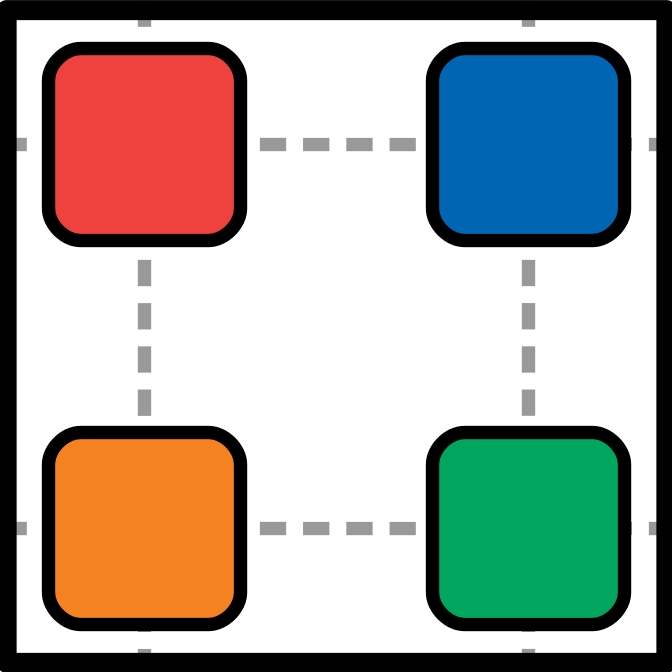
\includegraphics[width=0.09\textwidth]{IEEEtran/cyclic/gaols.jpg}}
 {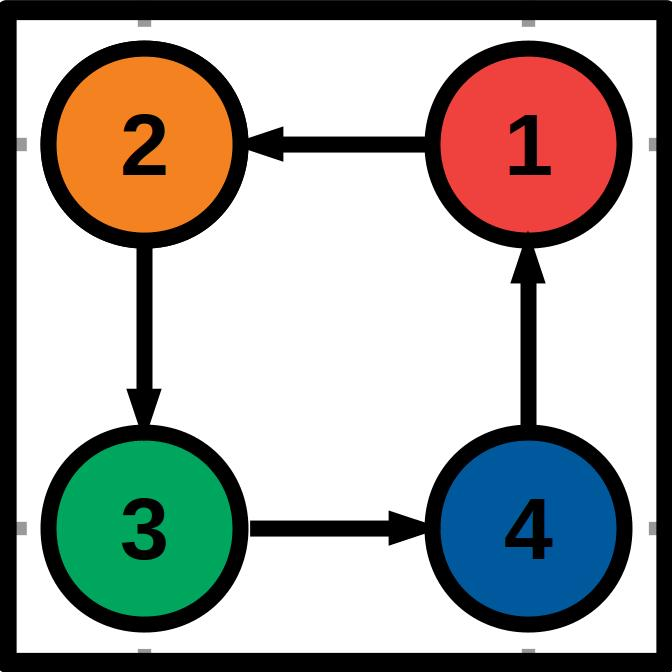
\includegraphics[width=0.09\textwidth]{IEEEtran/cyclic/c1.jpg}}
 {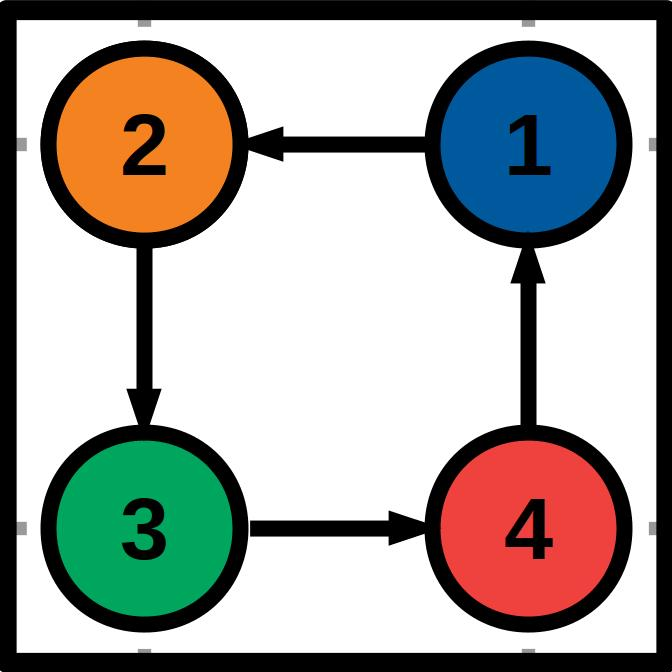
\includegraphics[width=0.09\textwidth]{IEEEtran/cyclic/c2.jpg}}
 {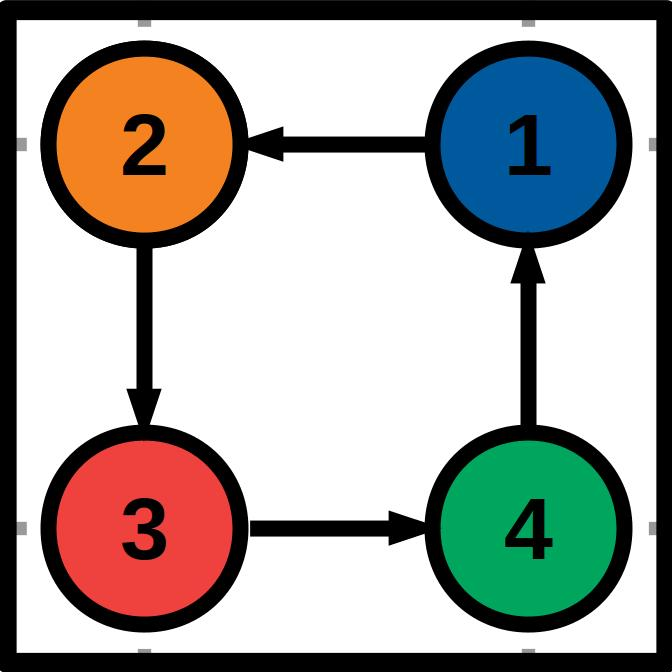
\includegraphics[width=0.09\textwidth]{IEEEtran/cyclic/c3.jpg}}
 {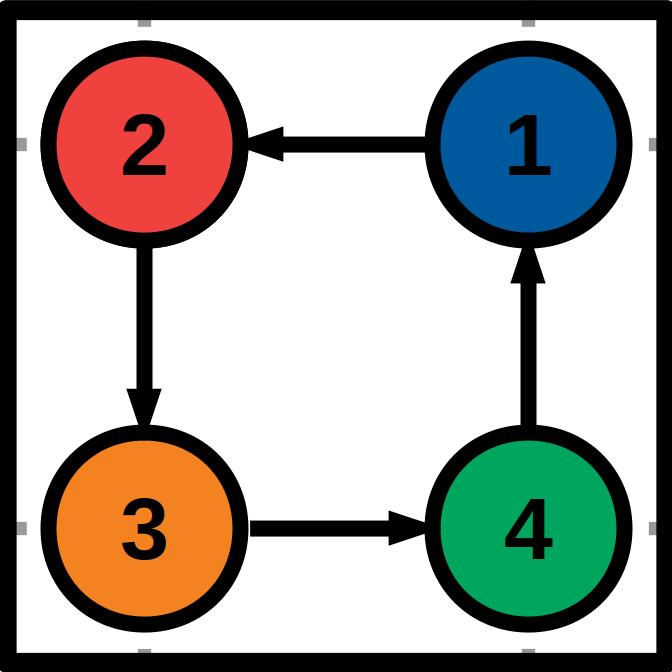
\includegraphics[width=0.09\textwidth]{IEEEtran/cyclic/c4.jpg}}
\caption{From left to right: A shape that contains 4 goal points; a sequence of events where $J_1$ strictly decreases. The frames of this sequence of events are ordered from left to right. All the information is encoded in the same way as Fig. \ref{fig:grid}.}
\label{fig:cyclic}
\end{figure}


\begin{itemize}
\item $\textit{\textbf{Case 2. The graph $\mathcal{G}_t$ is acyclic:}}$
\end{itemize}

If the $\mathcal{G}_t$ is acyclic, we can find at least one node whose out degree is 0 using vertex ordering. We call this type of nodes the \textit{head} agents. The \textit{head} agent can either be an agent that already arrived at the goal, or an agent that is still moving to the goal. If at least one \textit{head} has not arrived at its goal yet, $J_1$ will decrease by one because its next waypoint is open. Otherwise, if all the \textit{head}s have already arrived at their goal, then there is at least one agent who is blocked by a \textit{head} agent. Using \textit{Lemma} \ref{fact1}, we have that the blocked agent can make progress witha  non-zero probability by swapping with the \textit{head} that has already arrived at its goal. This action will either form a cycle, as shown in Fig. \ref{fig:acyclic} (\textit{right}), or generate a \textit{head} that hasn't reached its goal, shown in Fig. \ref{fig:acyclic} (\textit{left}), with at most $|A| - 1$ swaps. Hence in case 2, $J_1$ will decrease within a finite amount of time with non-zero probability as well.

\begin{figure}[H]
 \centering
{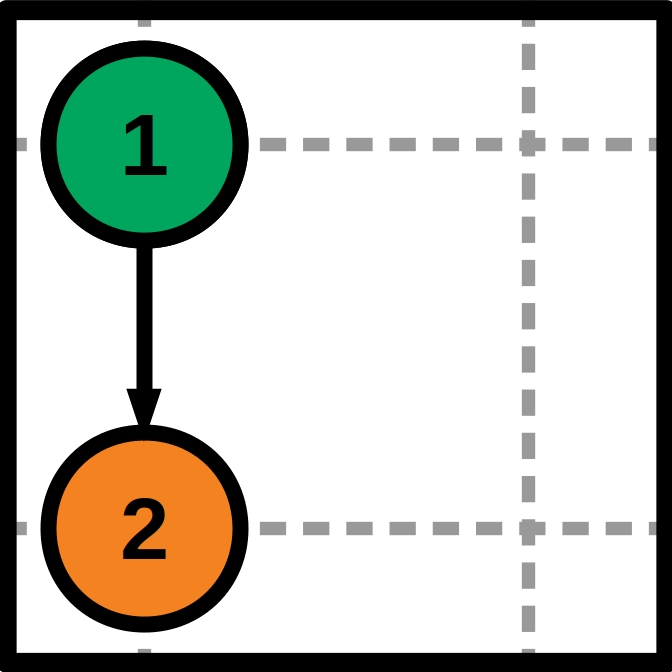
\includegraphics[width=0.09\textwidth]{acyclic/0.jpg}}
{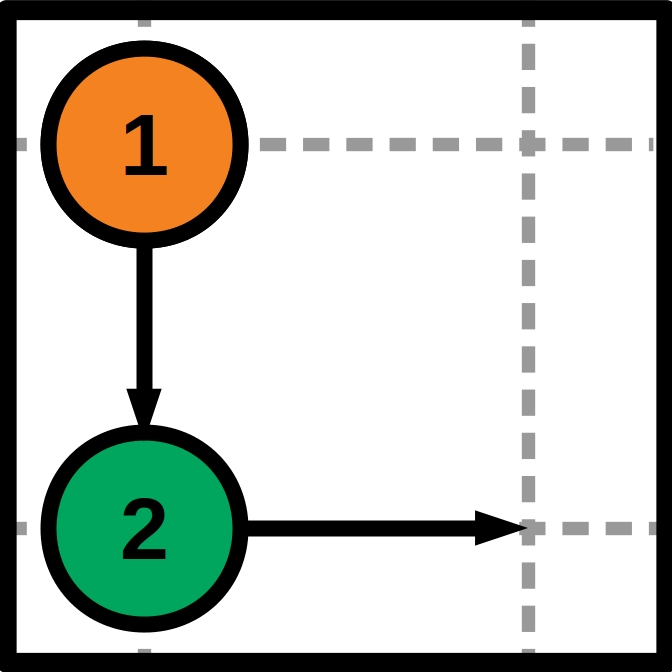
\includegraphics[width=0.09\textwidth]{acyclic/1.jpg}}\hfill
{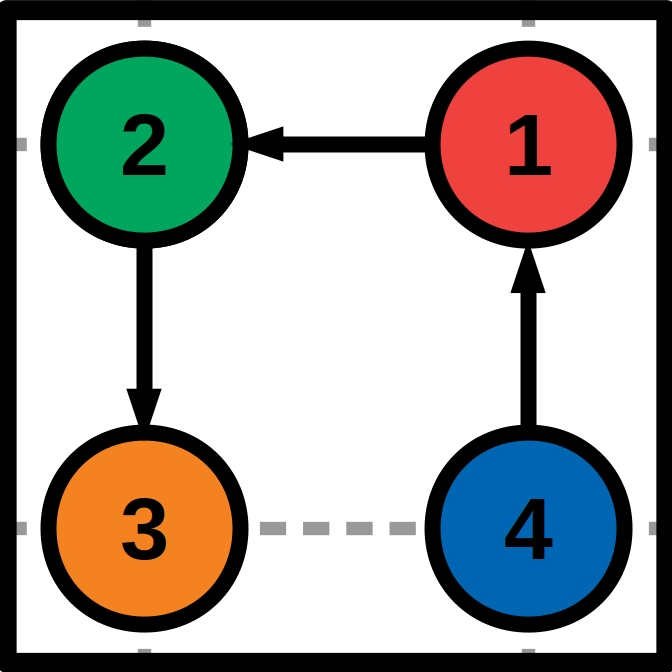
\includegraphics[width=0.09\textwidth]{acyclic/2.jpg}}
{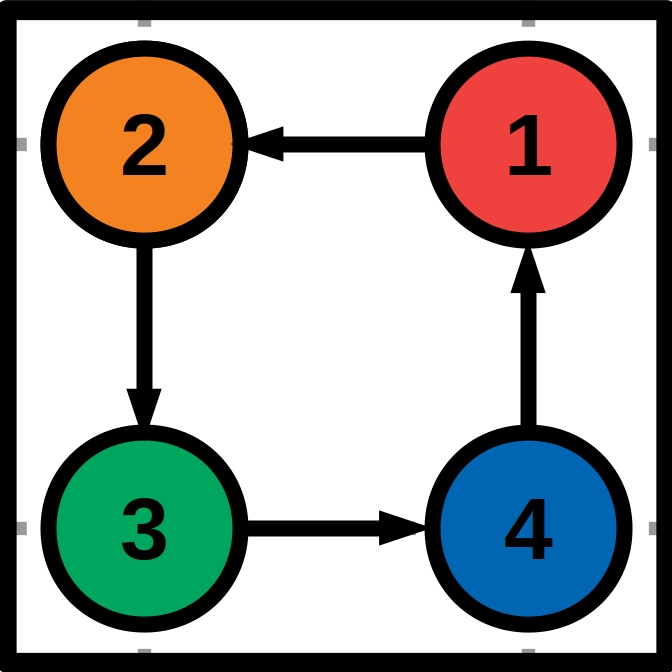
\includegraphics[width=0.09\textwidth]{acyclic/3.jpg}}
\caption{Illustration of two possible cases (shown by a sequence of two figures on the left and a sequence of two figures on the right) where \textit{head} has already arrived at its goal. The goal shape is shown in Fig. \ref{fig:cyclic} (\textit{left}). All the information is encoded in the same way as Fig. \ref{fig:grid}.}
\label{fig:acyclic}
\end{figure}
\end{proof}

\begin{lemma} 
The \textit{motion planner} will make the position of each assigned goal's owner to greedily move toward the position of the goal point with non-zero probability, regardless of the swarm's configuration.
\label{moves}
\end{lemma}
\begin{proof}
We prove this lemma via case analysis. At time $t$, for any agent $a$, let $q$ be $T_{a}(t)$, i.e., agent $a$'s target at time $t$. We here exhaustively outline all two possible cases:


\begin{itemize}
\item \textit{\textbf{Case 1. $a$ has not arrived at $q$:}}
\end{itemize}

If $a$ has not arrived at $q$, $a$ will intend to move to the next waypoint to get closer to $q$. If the waypoint is unoccupied, then $a$ moves one step closer to $q$. Otherwise, if the waypoint is occupied, using \textit{Lemma} \ref{fact1}, $q$ will be passed to the agent that is occupying the waypoint with non-zero probability. In either of these two cases, the distance between position of $q$'s owner and $q$ decreases by one with non-zero probability. 


\begin{itemize}
\item \textit{\textbf{Case 2. $a$ is already at $q$:}}
\end{itemize}

If $a$ is already at $q$, then $a$ can stay at $q$ with non-zero probability, completing the proof. 
\end{proof}
\begin{lemma}
If $J_2 \neq 0$, then the event that: two agents that are holding the same goal at the same time are located within distance $R$, will occur within a finite amount of time with non-zero probability. Namely, at time $\overline{t}$, if $J_2 \neq 0$, then $\exists ~\overline{\tau}, \overline{\epsilon} > 0, a_i \neq a_j,$ such that:
$$Pr\{||p_{a_i}(\overline{t} + \overline{\tau}) - p_{a_j}(\overline{t} + \overline{\tau})||\leq R, T_{ai}(\overline{t} + \overline{\tau}) = T_{aj}(\overline{t} + \overline{\tau})\} \geq \overline{\epsilon}$$
\label{lemmameet}
\end{lemma}

\begin{proof}\vskip -20pt
If $J_2\neq 0$, then at least two agents are holding the same goal point. Let $q_d$ be a goal which is assigned to more than one agent. \textit{Lemma} \ref{moves} is sufficient to show that two of $q_d$'s owners can concurrently keep moving greedily to $q_d$ with non-zero probability, shown in Fig. \ref{fig:meet} (\textit{left}), unless one of $q_d$'s owners blocks the other owner's way in the trip, shown in Fig. \ref{fig:meet} (\textit{right}). However, one agent being blocked by the other implies that the distance between two agents is one grid length, which is smaller than $R$, completing the proof.

\begin{figure}[h]
 \centering
 {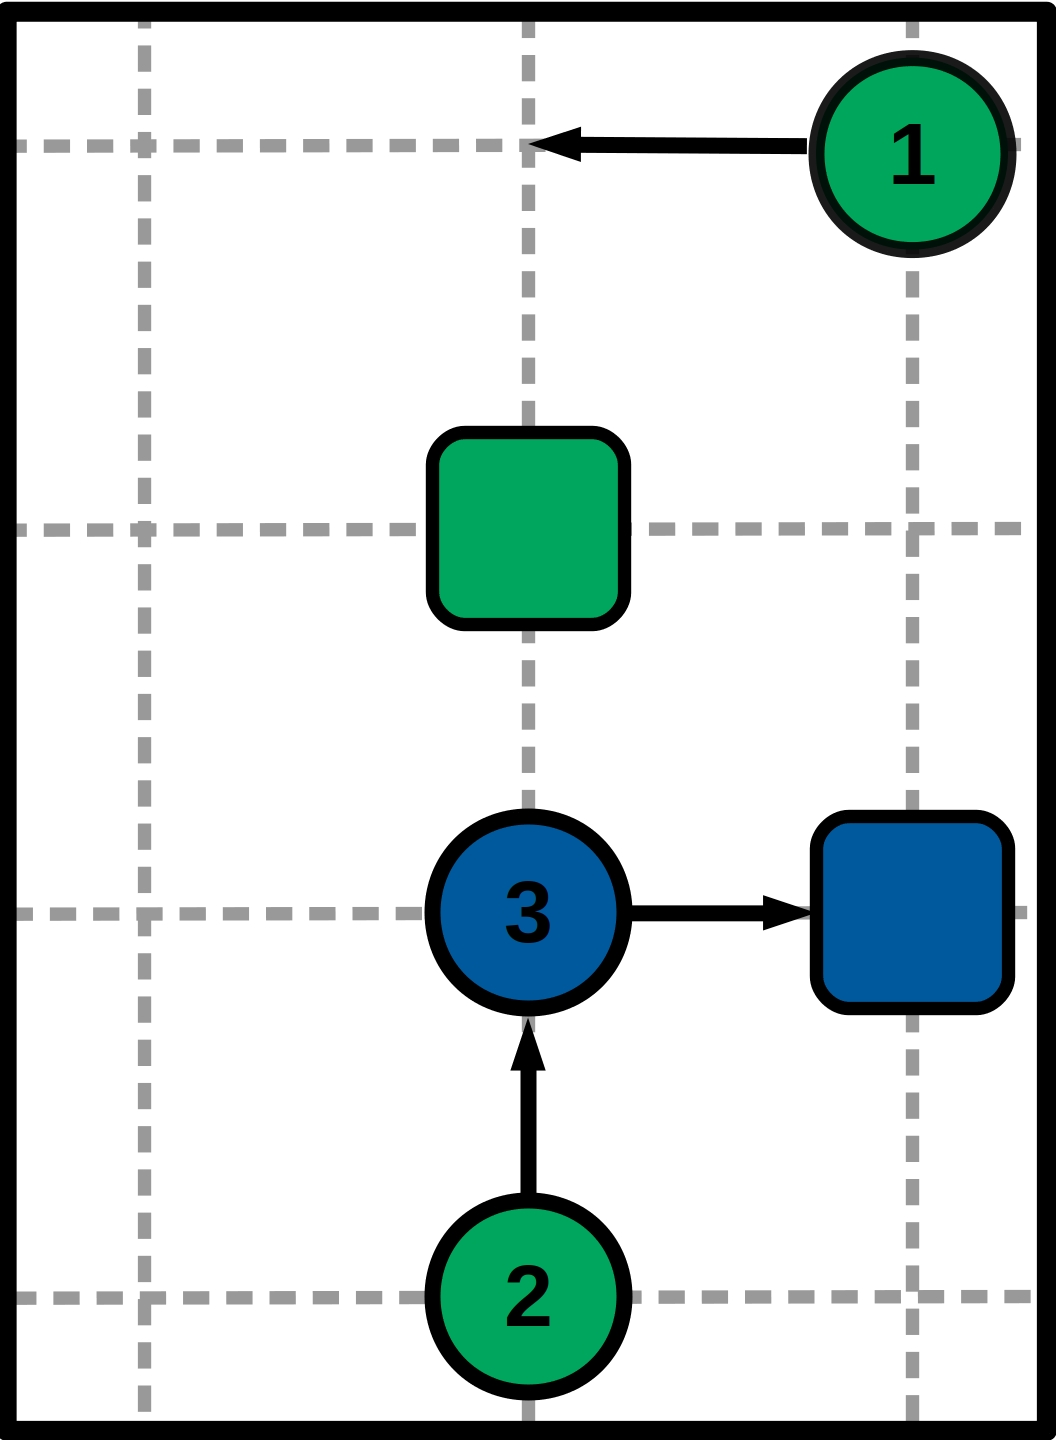
\includegraphics[width=0.135\textwidth]{meet/00.jpg}}
{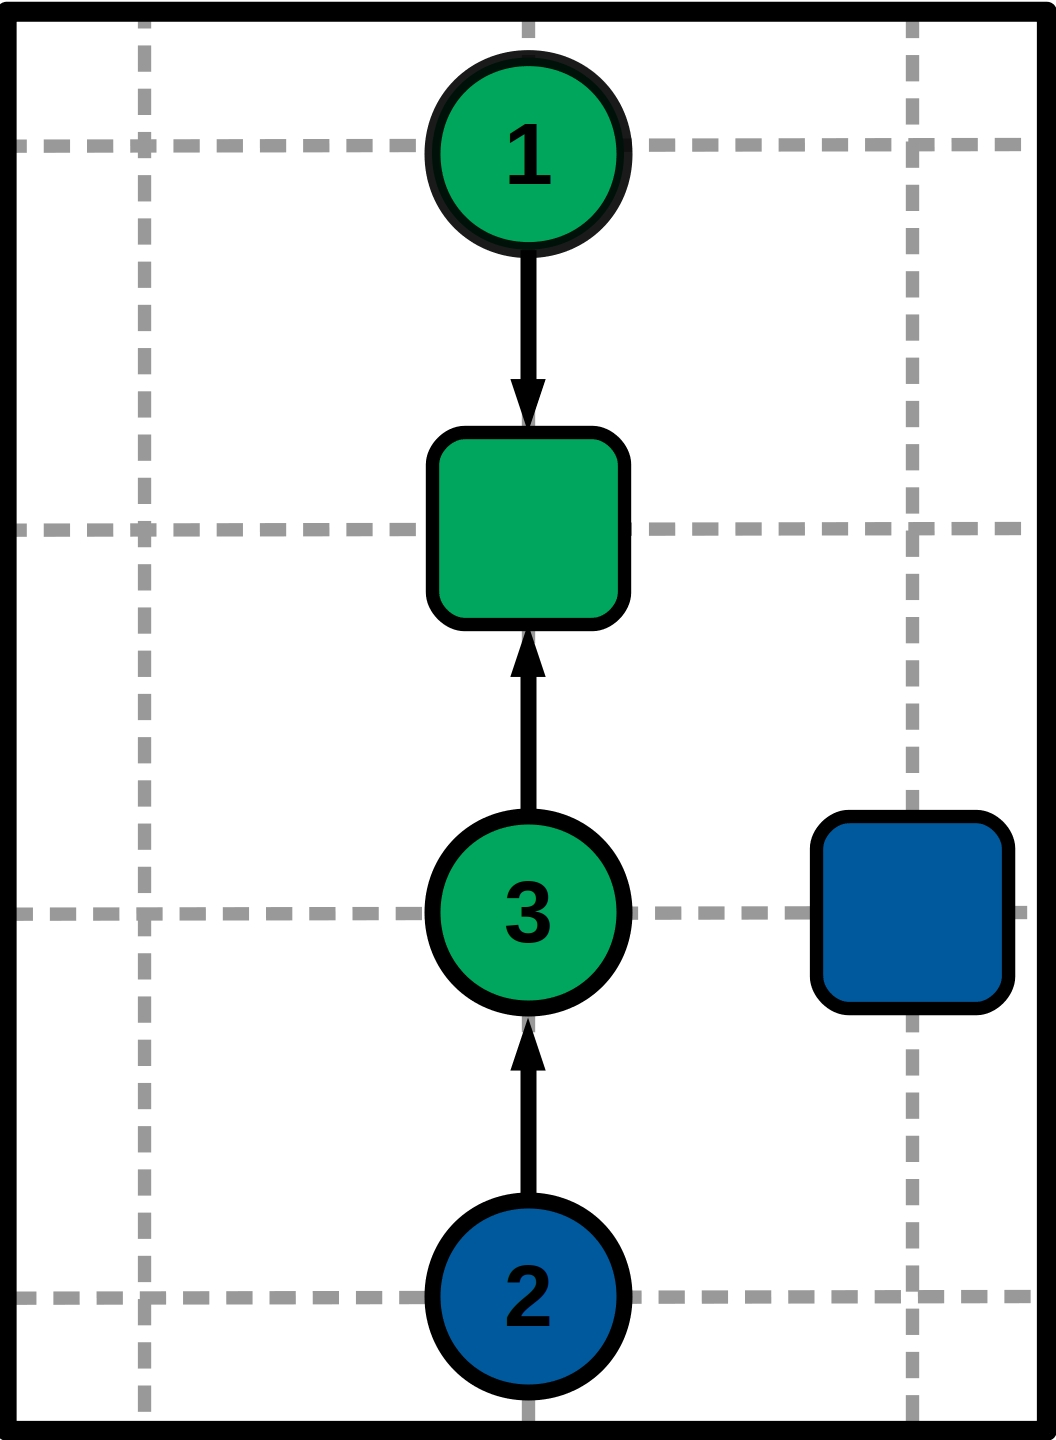
\includegraphics[width=0.135\textwidth]{meet/01.jpg}}\hfill\hfill\hfill\hfill
{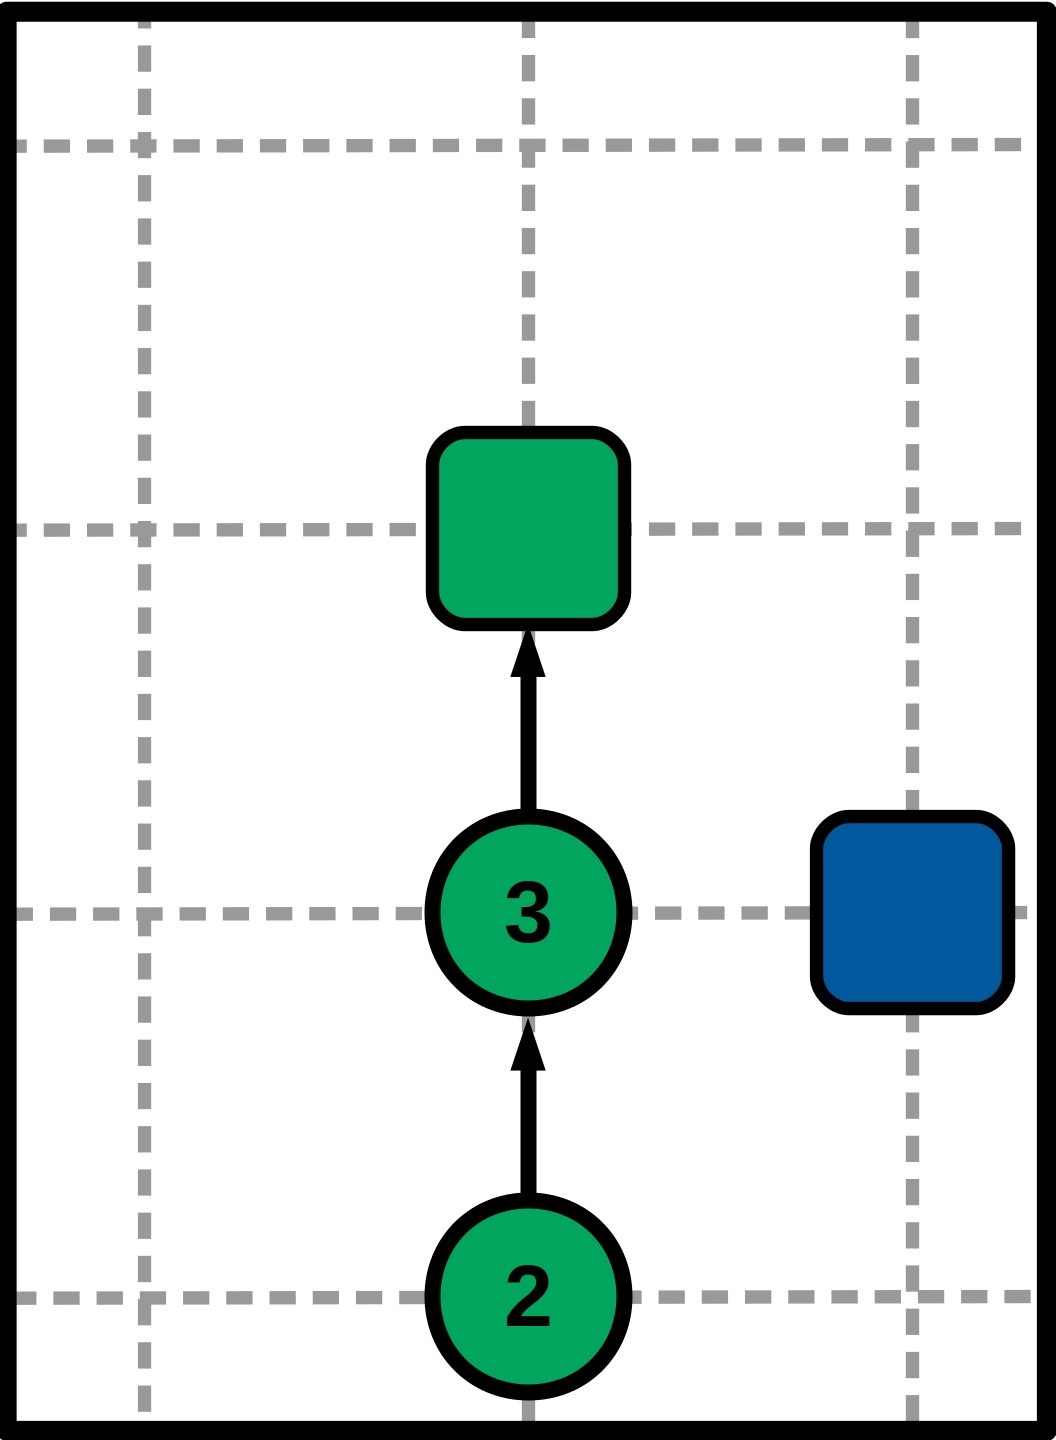
\includegraphics[width=0.135\textwidth]{meet/02.jpg}}
\caption{Illustration of two possible cases (shown by a sequence of three figures on the left and a single figure on the right) where two of $q_d$'s owners (circles in green) meet each other. All the information is encoded in the same way as Fig. \ref{fig:grid}.}
\label{fig:meet}
\end{figure}
\end{proof}

\begin{lemma} 
Let $\alpha$ be the probability that \textit{new goal selector} can pick a valid new goal point. If $J_2 \neq 0$ and $\alpha > 0$, then $J_2$ will decrease by at least one within a finite amount of time with non-zero probability, independent of the history.
\label{lemma4}
\end{lemma}

\begin{proof}
\textit{Lemma} \ref{lemmameet} suggests that if $J_2\neq 0$, then two agents holding the same goal will meet each other within a finite amount of time with non-zero probability, which means \textit{new goal selector} will be triggered within a finite amount of time with non-zero probability. Additionally, once \textit{new goal selector} is triggered, if $\alpha > 0$, then $J_2$ will decrease with non-zero probability, completing the proof. 
\end{proof}


\begin{theorem} 
Both $J_1$ and $J_2$ will almost surely converge to 0, regardless of the swarm's initial configuration.
\end{theorem}

\begin{proof}
Using \textit{Lemma} \ref{lemma1}, \ref{lemma2}, \ref{lemma3}, \ref{lemma4}, we can show that both $J_1$ and $J_2$ satisfy all three conditions proposed in \textit{Proposition} \ref{root}. Hence both $J_1$ and $J_2$ will almost surely converge to 0, regardless of the initialization of the swarm.
\end{proof}

\subsection{Complexity}
In the section, we study the cost of implementation of the algorithm using proposed in \ref{implementaion} with respect to its time complexity, memory complexity, and communication complexity. 

First, we study the time complexity for each agent planning their action, i.e., the time complexity for executing \textit{alg. \ref{alg:main} \textit{Line 9-35}}. One can see that the time cost is dominated by the time complexity for looping through all the messages received in last $\frac{2}{f_{comm}}$ amount of time. In the \textit{msg\_buff}, there will be at most $2|N_{a_i}(t)|$ amount of the messages, on the other hand, each agent can have at most $\lfloor{\frac{2R}{l}}\rfloor^2$ amount of neighbors in communication range, where $R$ is agent's communication range, $l$ is the grid length. This suffices to show that the time complexity for the decision making is $\mathcal{O}(\lfloor{\frac{R}{l}}\rfloor^2)$. 

Next, the algorithm's memory footprint is dominated by the memory to store the input point set, as a result, the algorithm's memory complexity is $\mathcal{O}(|Q|)$.

As to the communication complexity, in a unit of time, all the data that an agent $a_i$ needs to transmit to its neighbors is: $f_{comm}$ amount of broadcasting messages, and the data to swap the goal (communication cost for 2-way handshake). During a unit of time, one agent can broadcast $f_{comm}$ amount of messages and execute at most $f_{comm}|N_{a_i}(t)|$ amount of handshakes. This suffices to show that the amount of data transmitted during a unit of time is $\mathcal{O}(\lfloor{\frac{R}{l}}\rfloor^2 f_{comm})$, where $R$ is agent's communication range, $l$ is the grid length. 

\section{performance evaluation}
To demonstrate the correctness and performance of the algorithm presented in this paper, we implemented and tested it in both simulated and physical experiments. For all experimental tests, the shape was successfully formed.  We also compared the performance of our proposed algorithm with the centralized algorithm proposed in \cite{centralized}. In this centralized approach, every agent is initially assigned a unique goal.  In addition, this assignment minimizes the total traveling distance. It is shown in \cite{centralized} that with such optimal initial assignment, the agents' paths will form a acyclic direct graph (DAG), and the each agent's motion can be then scheduled via vertex ordering. Despite that the centralized method can produce the distance-optimal solution, which outperforms our method, it could suffer from a single-point of failure and therefore is less robust than our method.

\subsection{Simulation}

In simulation, each agent is modeled as an omni-directional robot equipped with GPS and a compass. We treat each agent as a circle with a radius of $0.05m$.  Agents are able to communicate with any other agent who lies within its communication range of $0.6m$, and travel at a speed of $0.05m/s$. These values match the physical robot described in section \ref{hardware}. 

In each test, the goal shape is given to the swarm in the form of a binary figure, i.e. a black and white image. The figure is scaled to make the number of goal pixels on the figure approximately equal to (always bigger than) the number of agents.  Example input images and corresponding shapes formed by the collective are shown in Fig. \ref{fig:tranform}. See Fig. \ref{fig:sim} for images from one simulation where 1024 agents formed the letters ``N" and ``U" in sequence.

\begin{figure}
{
\includegraphics[width=0.12\textwidth]{editor/grids/0.jpeg}}\hfill
{
\includegraphics[width=0.12\textwidth]{editor/grids/2.jpeg}}\hfill
{
\includegraphics[width=0.12\textwidth]{editor/grids/1.jpeg}}\hfill
{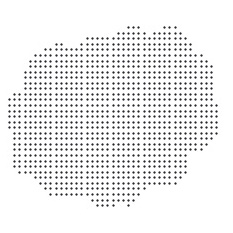
\includegraphics[width=0.12\textwidth]{editor/grids/3.jpeg}}

{
\includegraphics[width=0.12\textwidth]{editor/grids/test4.png}}\hfill
{
\includegraphics[width=0.12\textwidth]{editor/grids/test1.png}}\hfill
{
\includegraphics[width=0.12\textwidth]{editor/grids/test3.png}}\hfill
{
\includegraphics[width=0.12\textwidth]{editor/grids/test2.png}}\hfill
\caption{1024 agents form four user-defined shapes. (Bottom) example input binary images and (top) corresponding collective formations.}
\label{fig:tranform}
\end{figure}



\begin{figure*}[t]
 \centering
 \subfloat[T = 0s\label{fig:frame1}]{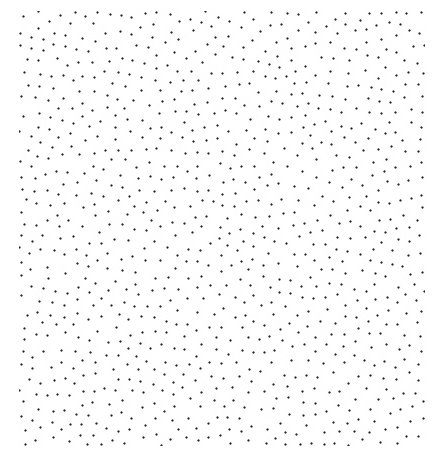
\includegraphics[width=0.245\textwidth]{frames/0.jpeg}}\hfill
\subfloat[T = 99s\label{fig:frame2}]{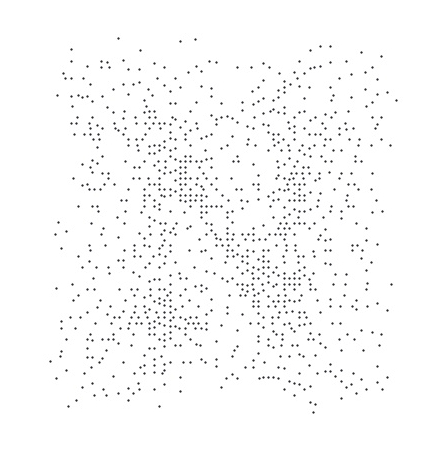
\includegraphics[width=0.245\textwidth]{frames/99.jpeg}}\hfill
\subfloat[T = 147s\label{fig:frame3}]{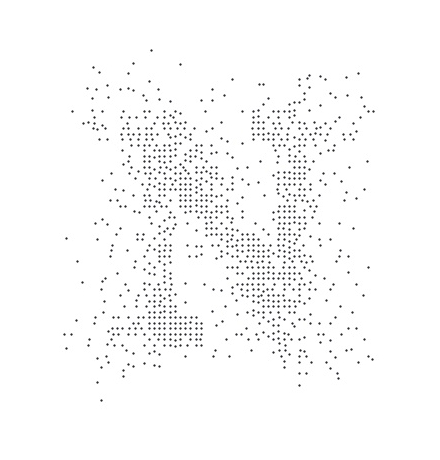
\includegraphics[width=0.245\textwidth]{frames/147.jpeg}}\hfill
\subfloat[T = 838s\label{fig:frame4}]{
\includegraphics[width=0.245\textwidth]{frames/838.jpeg}}
\\
\subfloat[T = 877s\label{fig:frame5}]{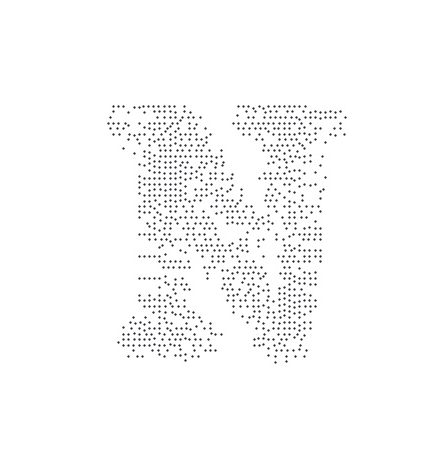
\includegraphics[ width=0.245\textwidth]{frames/877.jpeg}}\hfill
\subfloat[T = 888s\label{fig:frame6}]{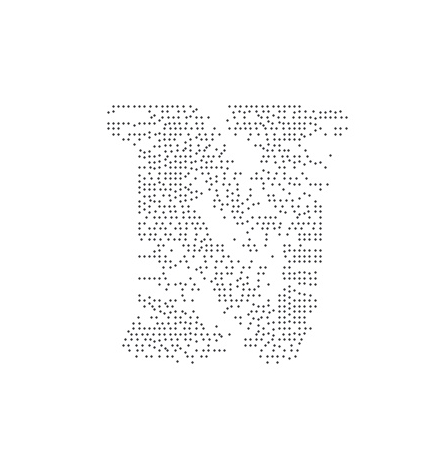
\includegraphics[width=0.245\textwidth]{frames/888.jpeg}}\hfill
\subfloat[T = 906s\label{fig:frame7}]{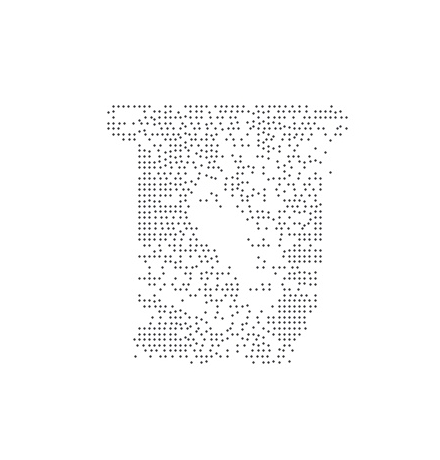
\includegraphics[width=0.245\textwidth]{frames/906.jpeg}}\hfill
\subfloat[T = 1031s\label{fig:frame8}]{
\includegraphics[width=0.245\textwidth]{frames/1031.jpeg}}\hfill

\caption{Still images from simulation where 1024 agents try to form two different shapes in a row. In this simulation, a swarm of 1024 agents first form a letter "N", then switch to a letter "U" when it is detected that all robots have reached an goal.}
\label{fig:sim}
\end{figure*}

First, the simulation is used to investigate the effect of the swarm size on the algorithm's convergence time, i.e. the total time it takes for the swarm to complete shape formation, as well as average robot travel distance, i.e., the total distance traveled by all robots normalized by the number of robots. In this task, swarms of size 16 to 529 agents formed a given target configuration from a random initialization. For every swarm size, 200 trials were run, and in each trial the target shape is randomly generated as a set of connected random positions. The large number of trials are able to eliminate the bias on the final result that is introduced by the target shape, since in each trial the target shape is randomly generated. Fig. \ref{fig:mesh1} shows the distributions of convergence time as well as the average distance traveled for different swarm sizes, and a comparison to the centralized method  \cite{centralized}. One counter-intuitive observation here is that the convergence time for centralized methods does not monotonically increase over the swarm size, sometimes even goes down. It is shown in \cite{centralized} that the worst case convergence time for centralized method is $|A|+d_{max}-1$ where $|A|$ is the number of agents, and $d_{max}$ is the maximal individual travel distance (the distance from one agent's initial position to its goal) amongst swarm. On the other hand, in simulations, the swarm moved in a fixed-size arena, hence when swarm size $|A|$ increases, i.e., the density of the swarm increases, the $d_{max}$ will decrease, as a result, the convergence time for centralized methods will not necessarily increase over the swarm size. The fact that agents move in a fixed-size arena can also help to explain the trend of the total distance plots. As the $|A|$ goes up, the swarm's initial position will be ``closer" to the target positions (one can consider an extreme case where number of the agents equals to the number of the vertices in arena, in this case, the average distance traveled will be 0), hence the overall trend of the distance plot is that the average distance traveled goes down as number of agents goes up. In these plots, we can see that the distance traveled incurred by our method is only around $20\%$ more than the one that is incurred by the centralized method. Moreover, when the density of the swarm is low ($\leq$ 225 agents in arena), the difference on convergence times for both methods are considerably small. When the density of the swarm increase, the convergence time for our method sharply increases, this is because in this case, the random goal swaps, i.e., the goal swaps to resolve the deadlock, will more likely happen, as a result, the algorithm will converge slower.  





\begin{figure}[h!]
    \centering
    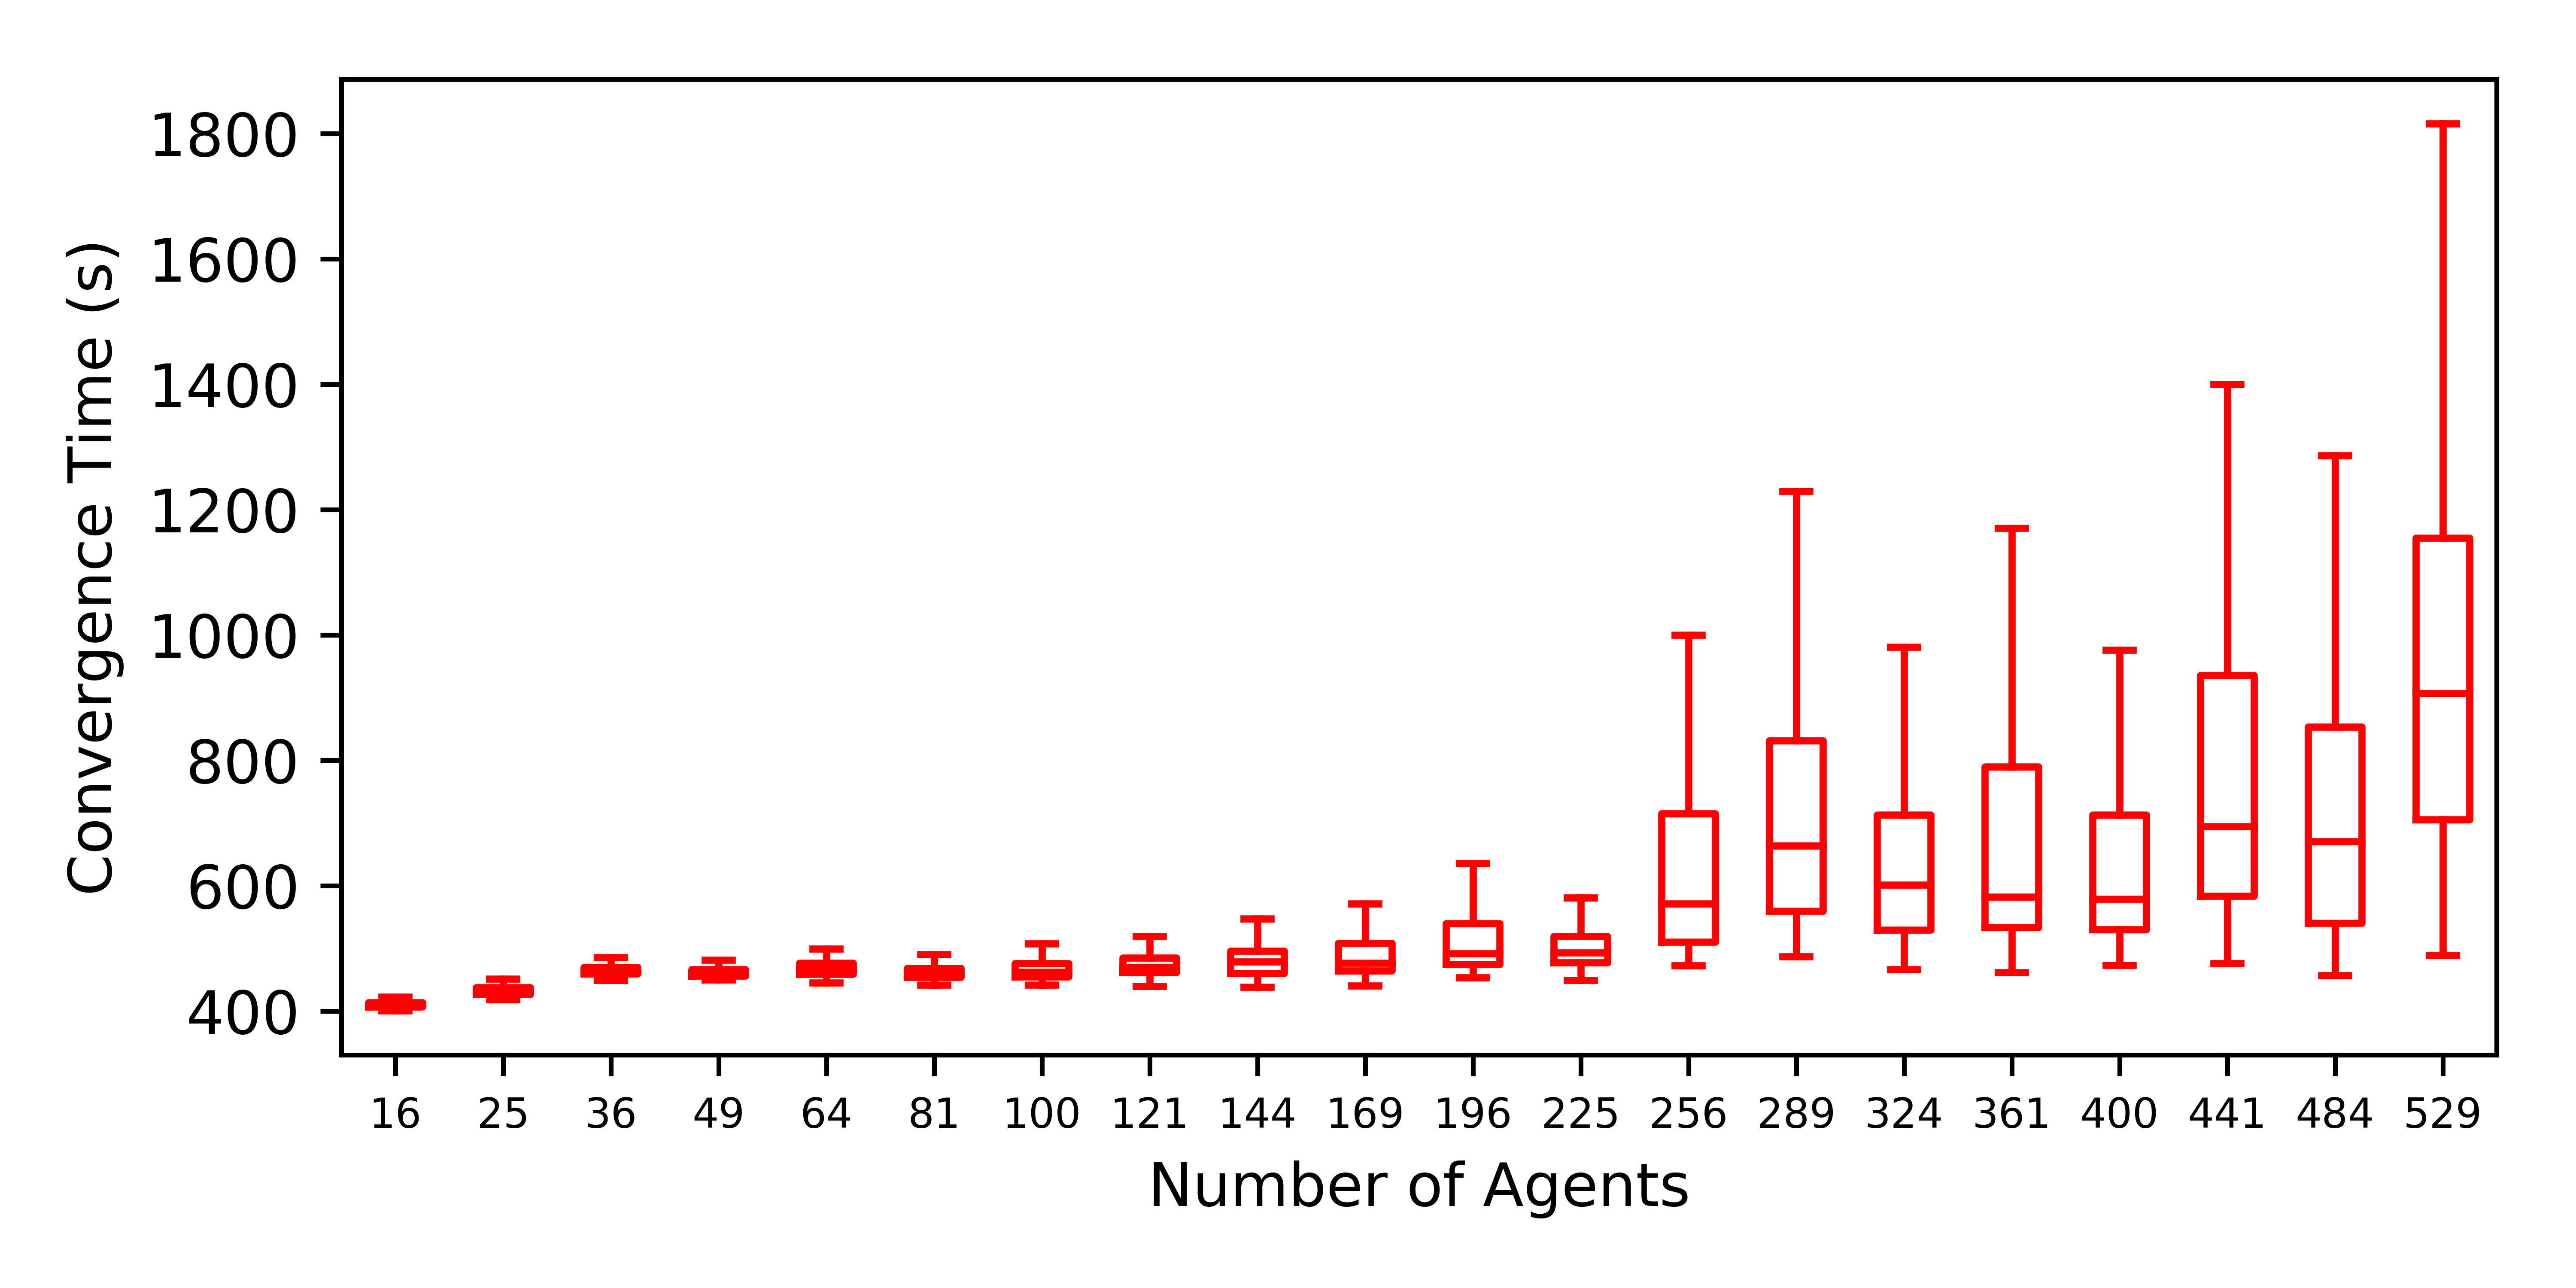
\includegraphics[trim=11pt 10pt 10pt 8pt, clip, width=0.48\textwidth]{variance/time_our.png}
    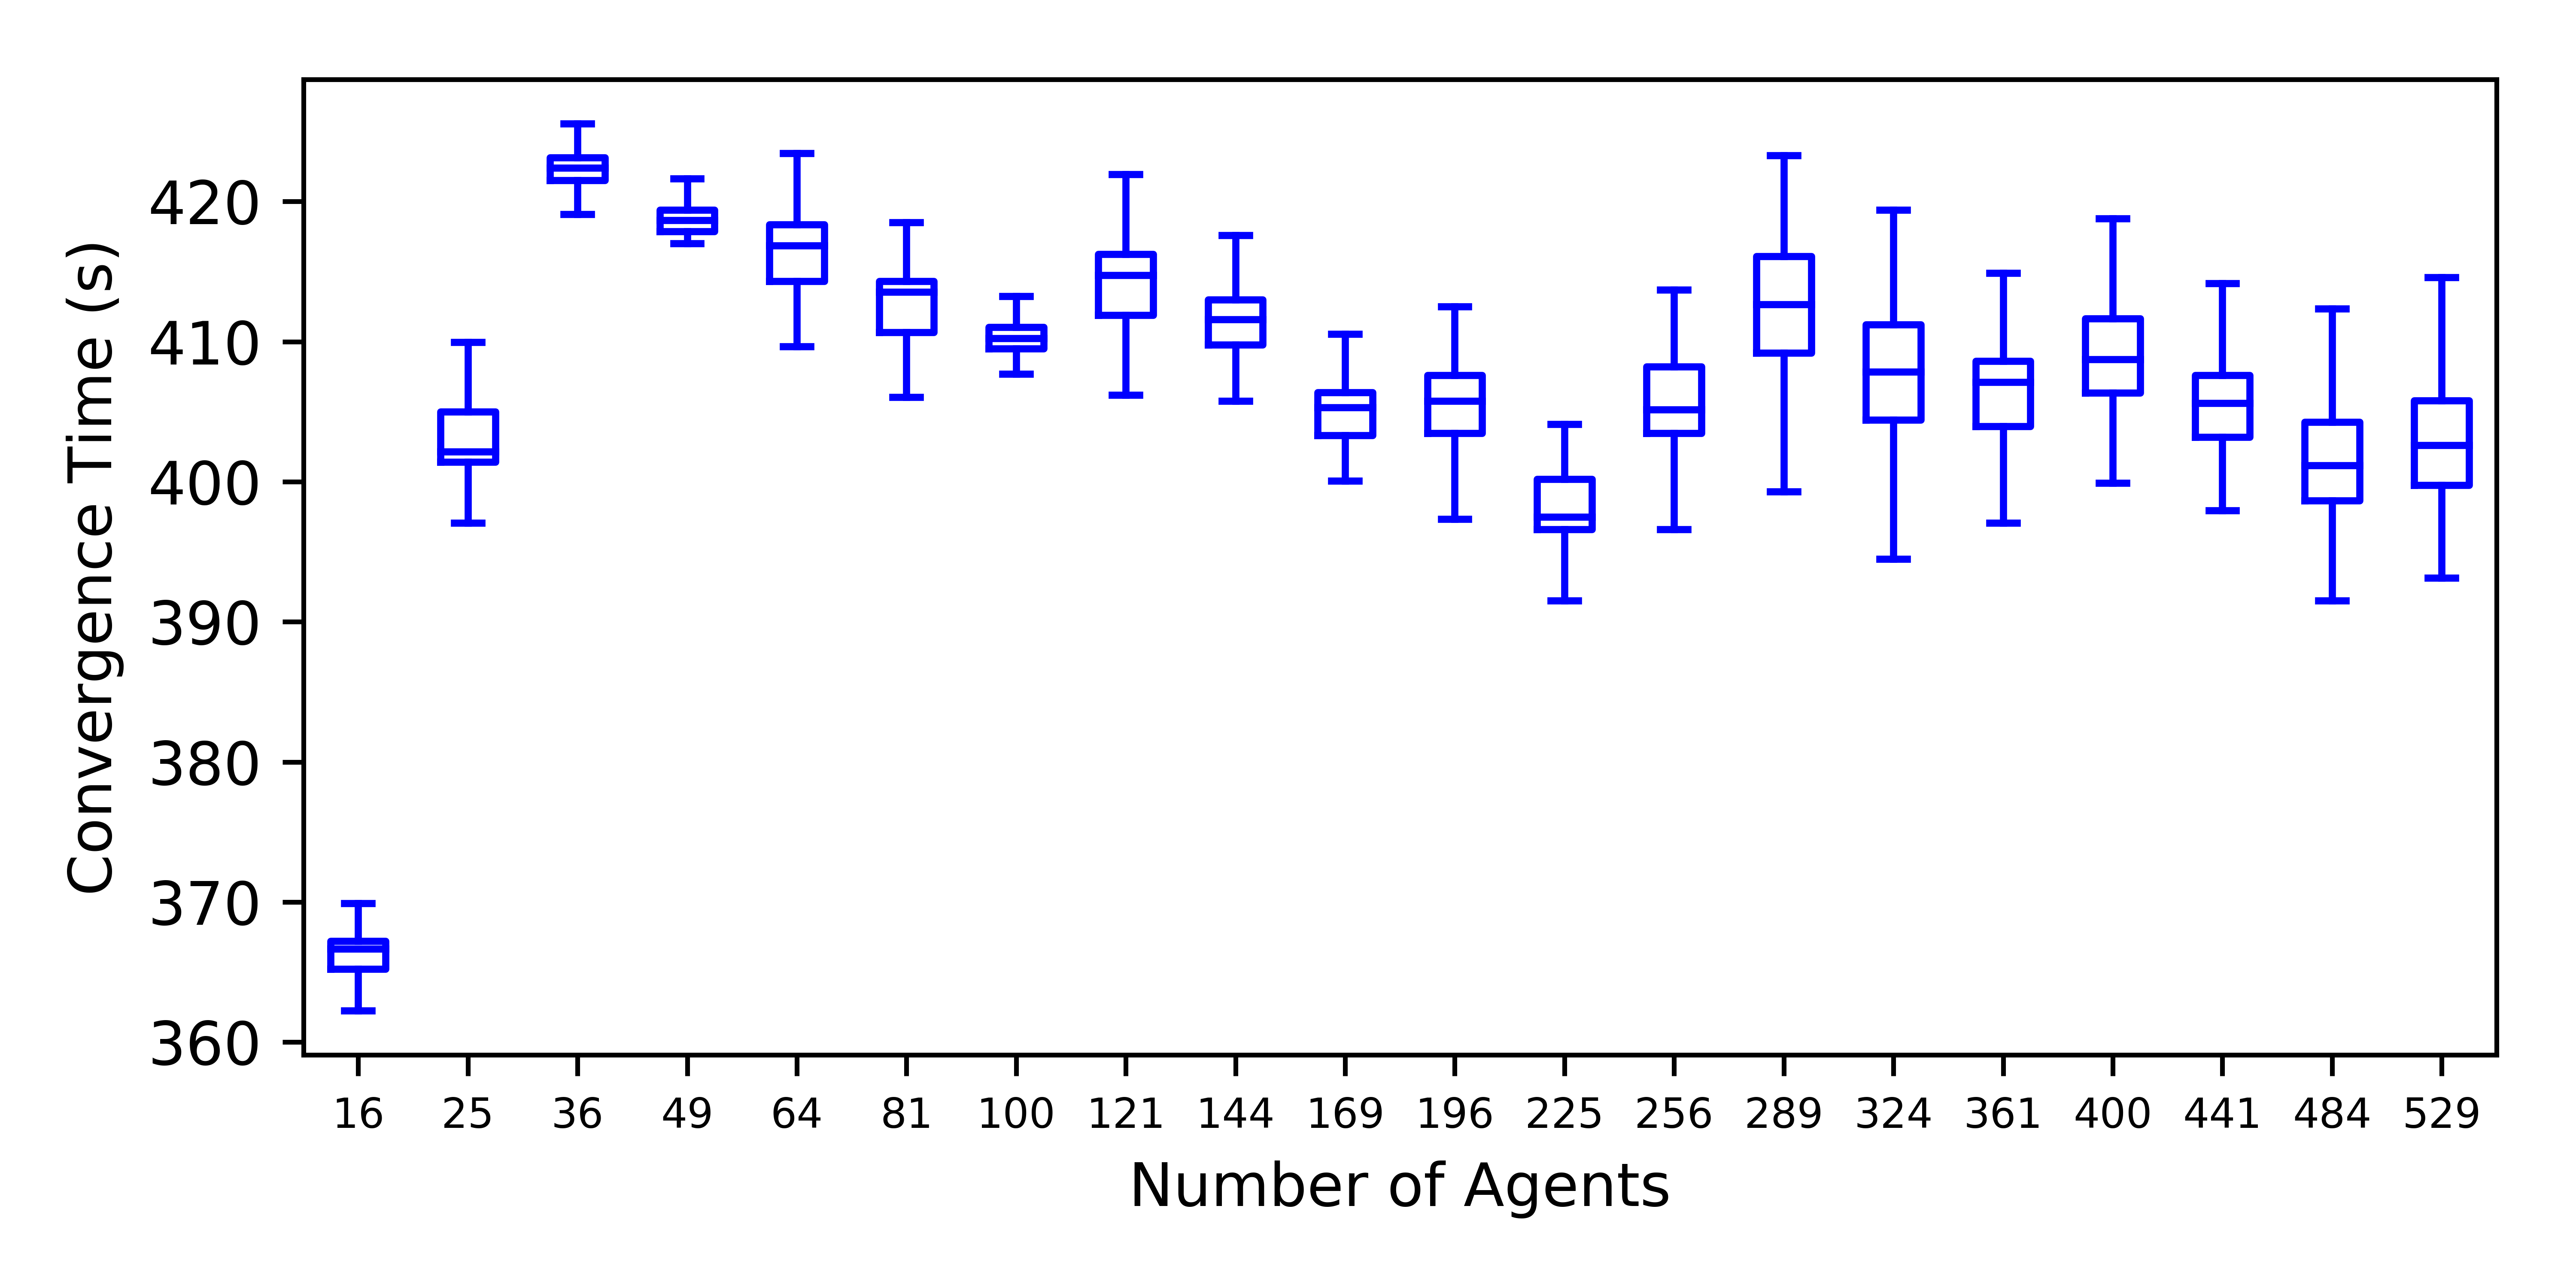
\includegraphics[trim=10pt 10pt 10pt 5pt, clip,width=0.48\textwidth]{variance/time_opt.png}
    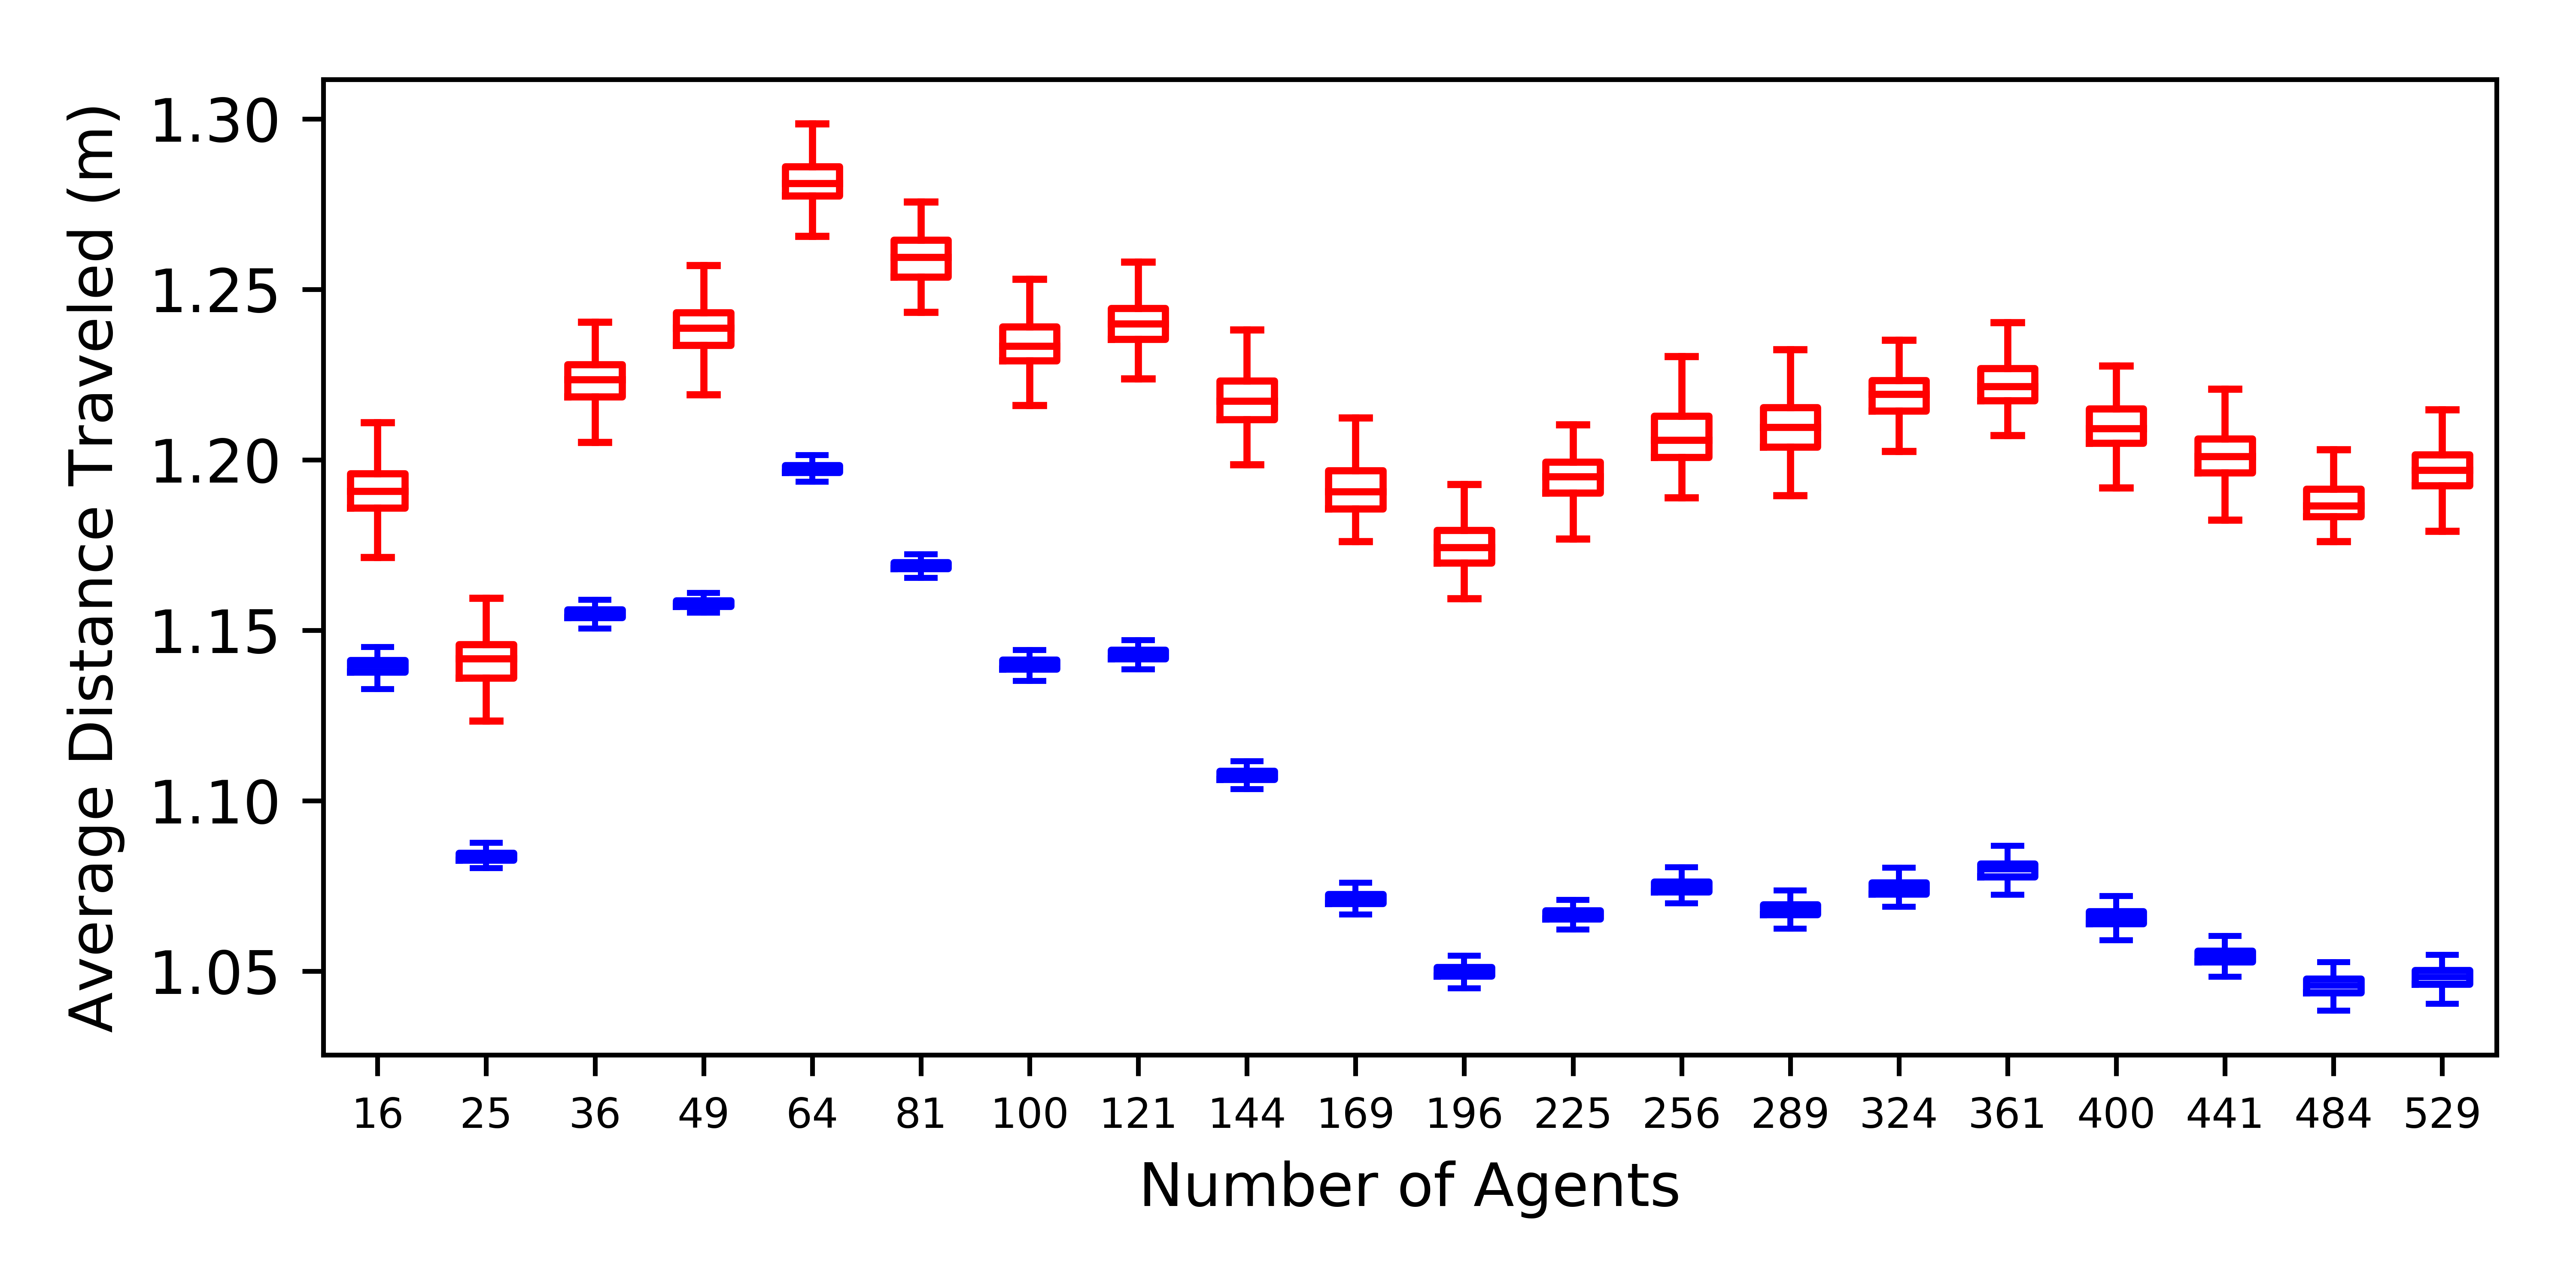
\includegraphics[trim=10pt 10pt 10pt 5pt, clip,width=0.48\textwidth]{variance/distance_our.png}
    \caption{Simulation results for both our method and the centralized method \cite{centralized} in standard box-plot format. The data in red is from our method and the data in blue is from the centralized method. For each number of agents, 200 trials were run, and in each trial the target shape was randomly generated. }
    \label{fig:mesh1}
\end{figure}

A second test compares the two approaches for \textit{new goal selector}.  It measures the convergence rate as well as the total distance traveled by a fixed-size swarm. In this experiment, 400 agents try to form 200 different randomly generated shapes. For each shape, the swarm executes the formation algorithm 200 times, giving a total of 40,000 simulation runs.  For each of these runs, agents are initialized with a uniform random distribution centered at the shape's center of mass. For every time step, we measure the average completion rate , the average distance traveled, and the confidence interval at a confidence level of $2\sigma$ for both convergence and distance travel, at that time for all 40,000 runs. The results are shown in Fig. \ref{fig:mesh2}. In these plots, we can see that the gradient based selector can dramatically increases the algorithm's convergence rate and helps to eliminate the long tail of convergence incurred by the random goal selector. Besides that, unsurprisingly, the gradient based goal selector can also help to make the algorithm more deterministic. 

\begin{figure}[h!]
{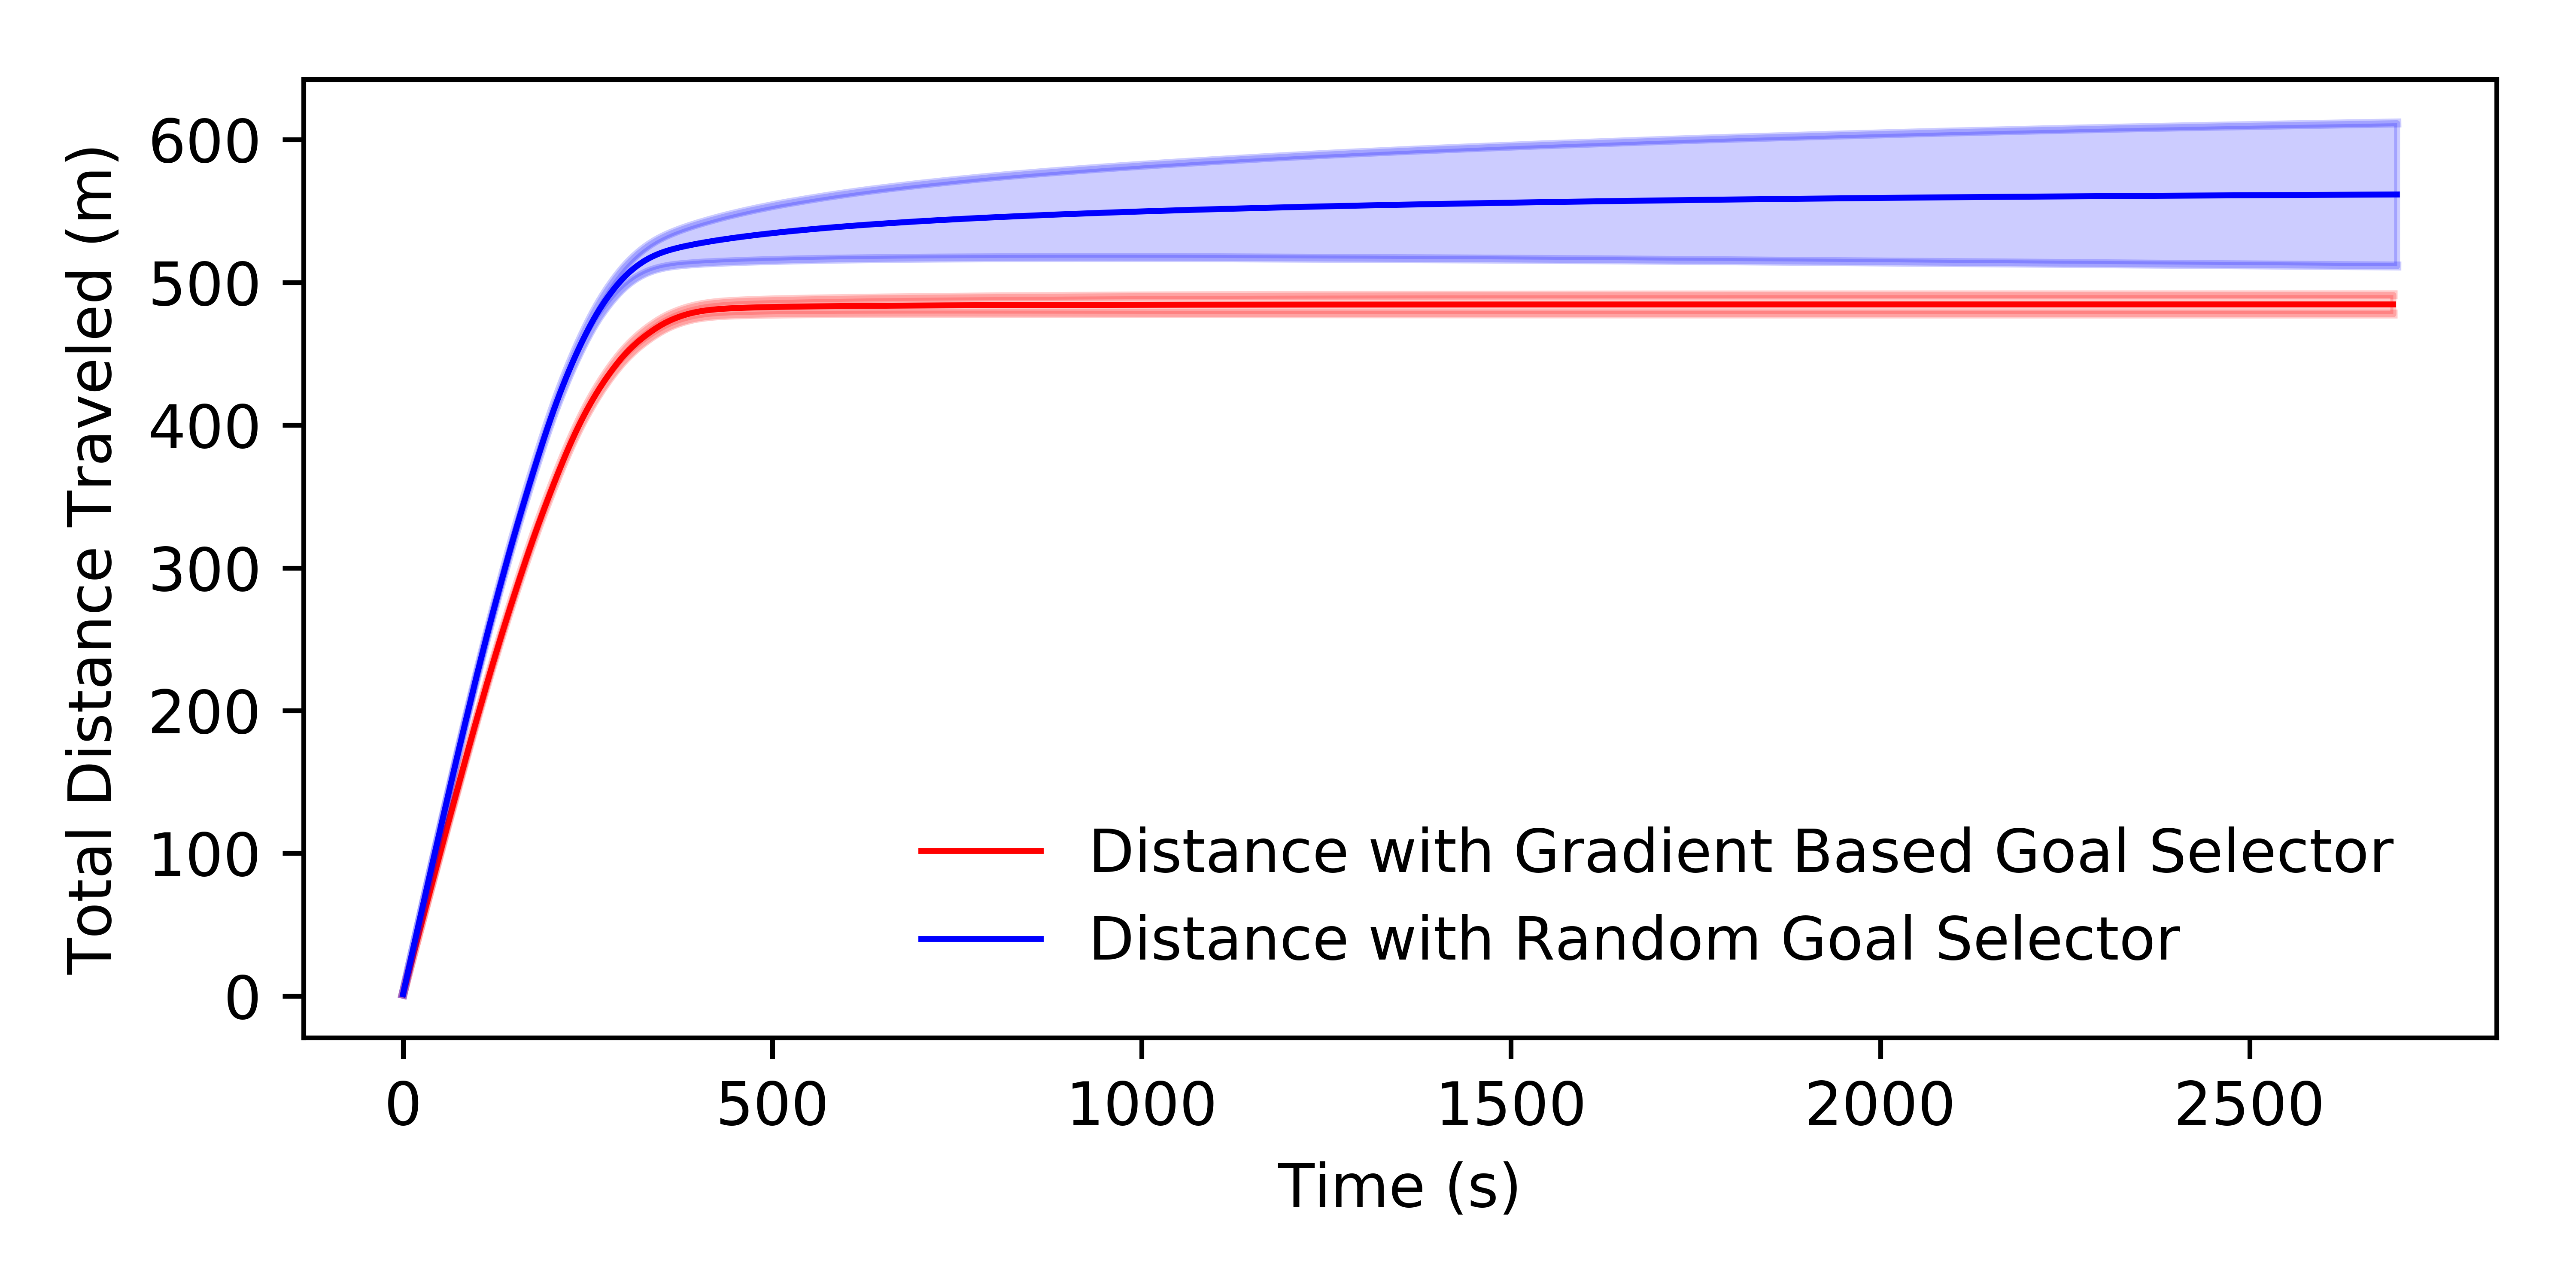
\includegraphics[trim=10pt 10pt 10pt 5pt, clip,width=0.48\textwidth]{IEEEtran/comparison/random/comparison_random_tro_dis.png}
\\
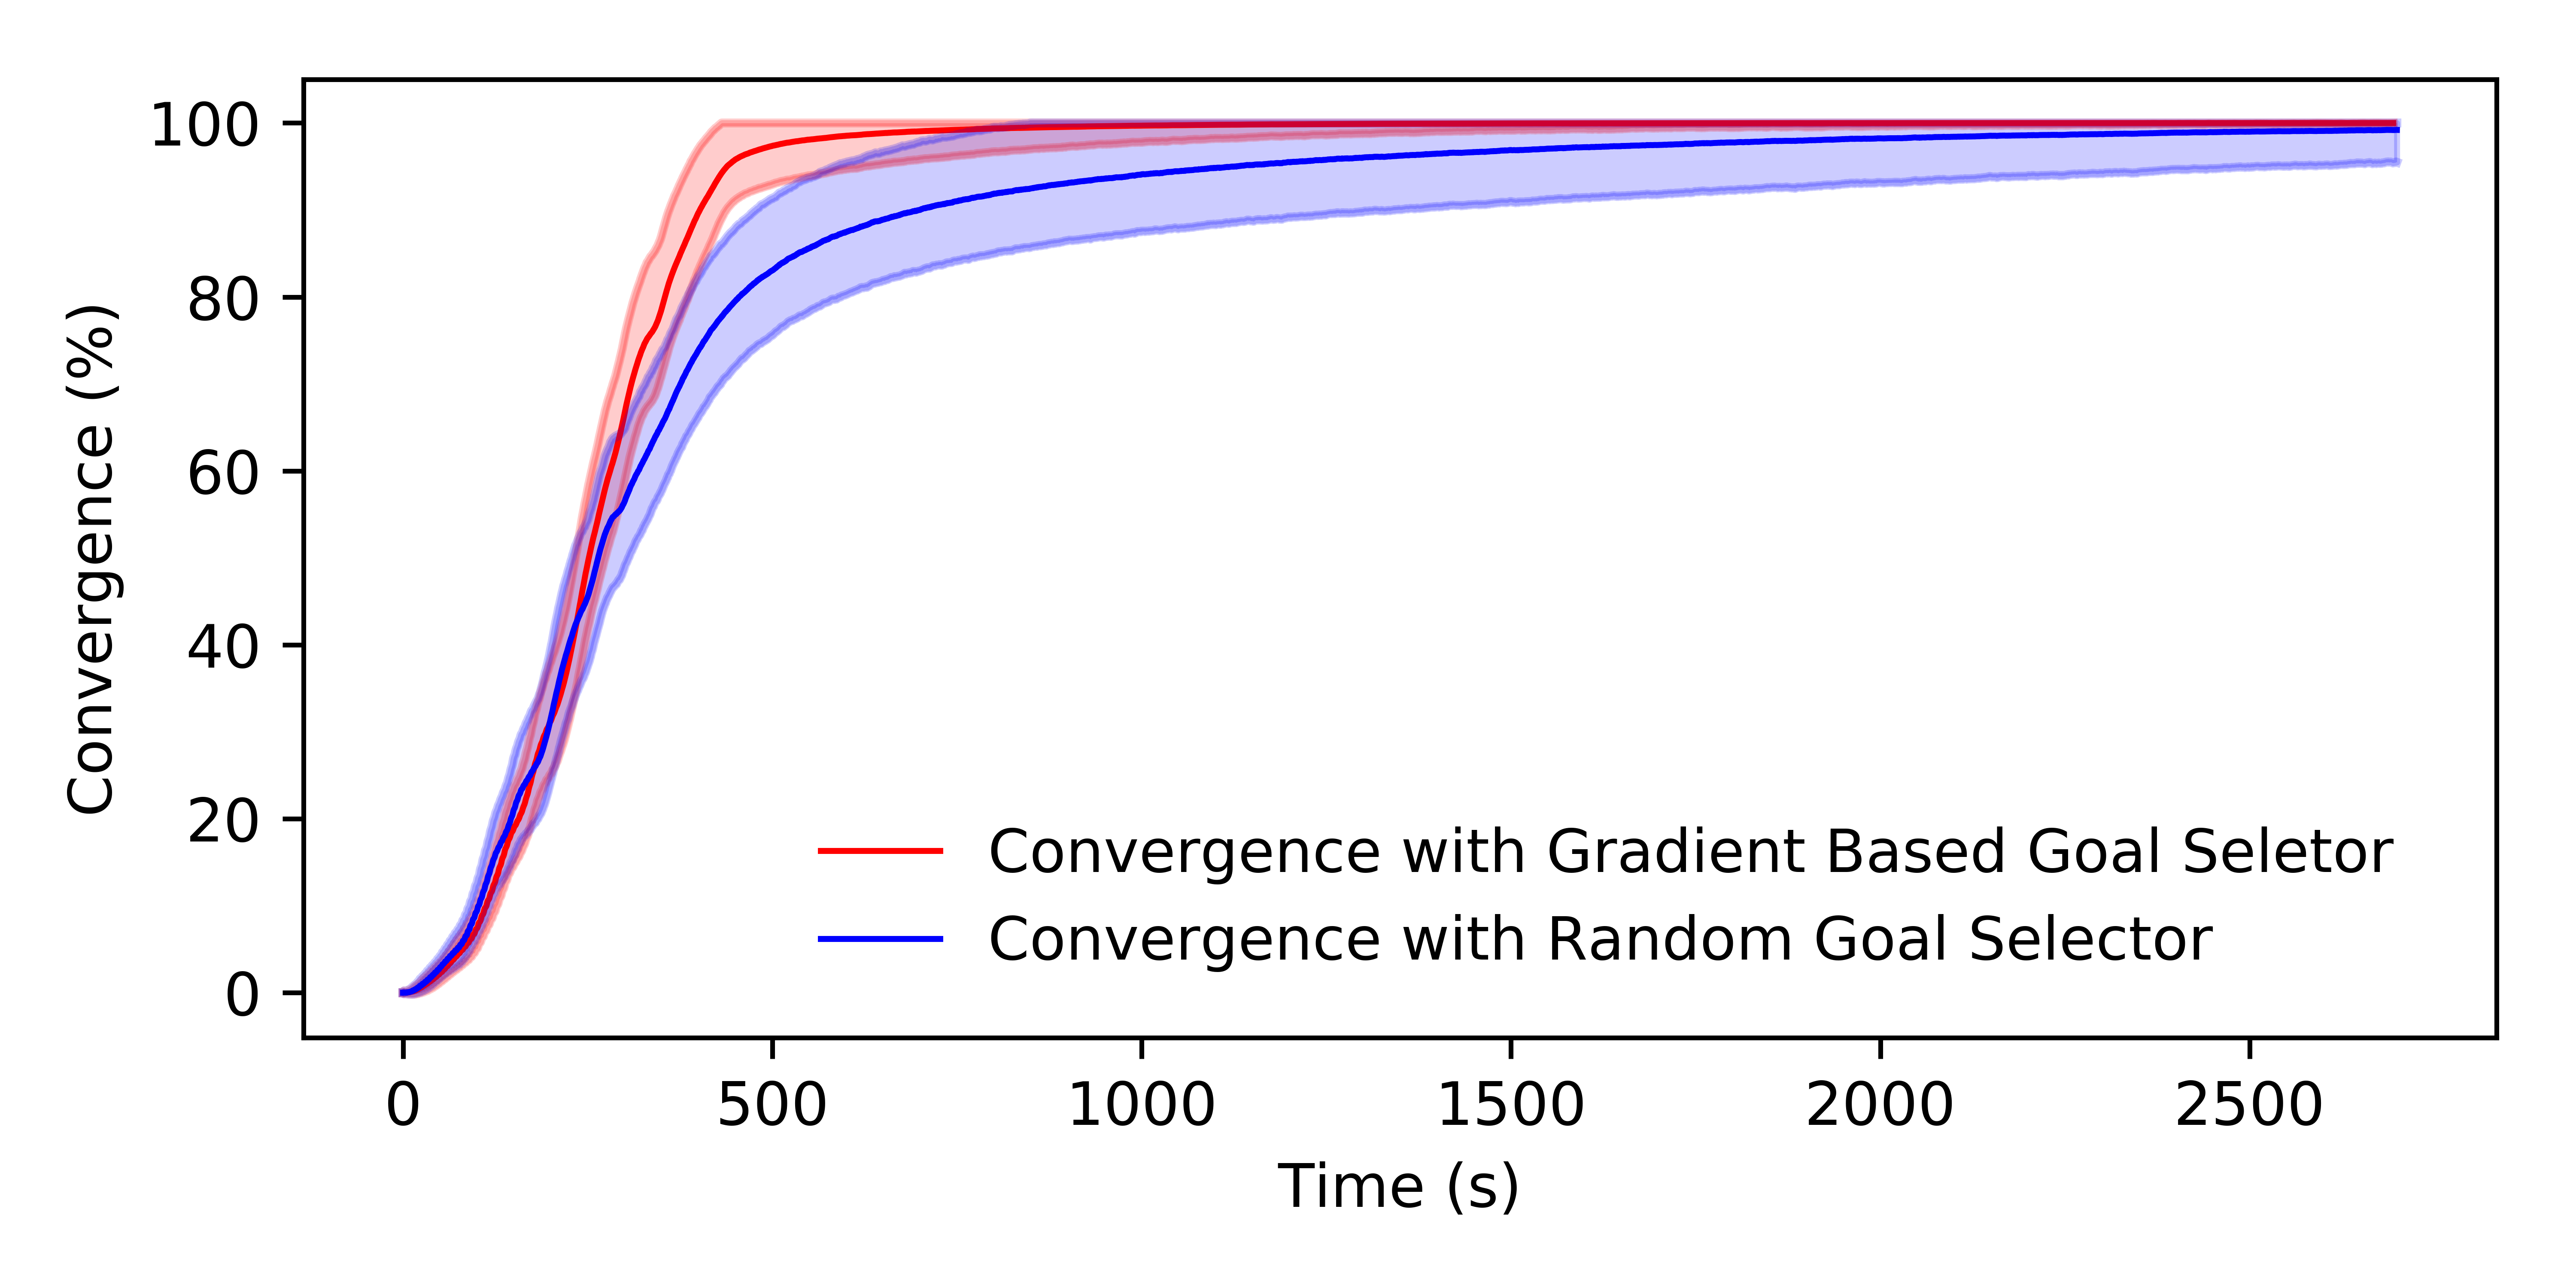
\includegraphics[trim=10pt 10pt 10pt 5pt, clip, width=0.48\textwidth]{IEEEtran/comparison/random/comparison_random_tro.png}
}
 \caption{
 Illustration of the improvement made by the gradient based selector on the algorithm convergence rate and total distance traveled compared to using a random selector. Each solid line in the plot is the average result from 40,000 simulations of 400 agents, and the colored shade areas show the confidence interval for convergence and total distance traveled over time at a confidence level of 2$\sigma$ (two standard deviations above or below the average).}
 \label{fig:mesh2}
\end{figure}

Simulation was also used to compare the convergence rate as well as swarm's total traveled distance for both our method and the centralized one. The experiment contains 40,000 trials; in every trial, 400 agents tried to drive toward a set of randomly generated goal points. First, agents were initialized with random starting locations. Next, either our method or the centralized method was used to drive the agents to the goal points. The simulation results of our method and the centralized method are shown in the Fig. \ref{fig:1222}. The difference between Fig. \ref{fig:1222} and Fig. \ref{fig:mesh1} is that: Fig. \ref{fig:mesh1} shows the statistics of final solution's quality, i.e., the total distance and convergence time, whereas the Fig. \ref{fig:1222} helps us to understand how does the algorithm's convergence and distance traveled change over time. The plot shows average result and the confidence interval with a confidence level of $2\sigma$ for both the convergence rates and total distance traveled for both methods. Note that at the beginning, from time 0s to 80s, our algorithm makes faster progress than the centralized method.  This is because in the centralized method, agents take goals located in the inner area of the shape first so they will not block other moving agents' paths, while in our method, agents initially choose goals at random.  Therefore our method gets a short-term win at the beginning.

\begin{figure}[h!]
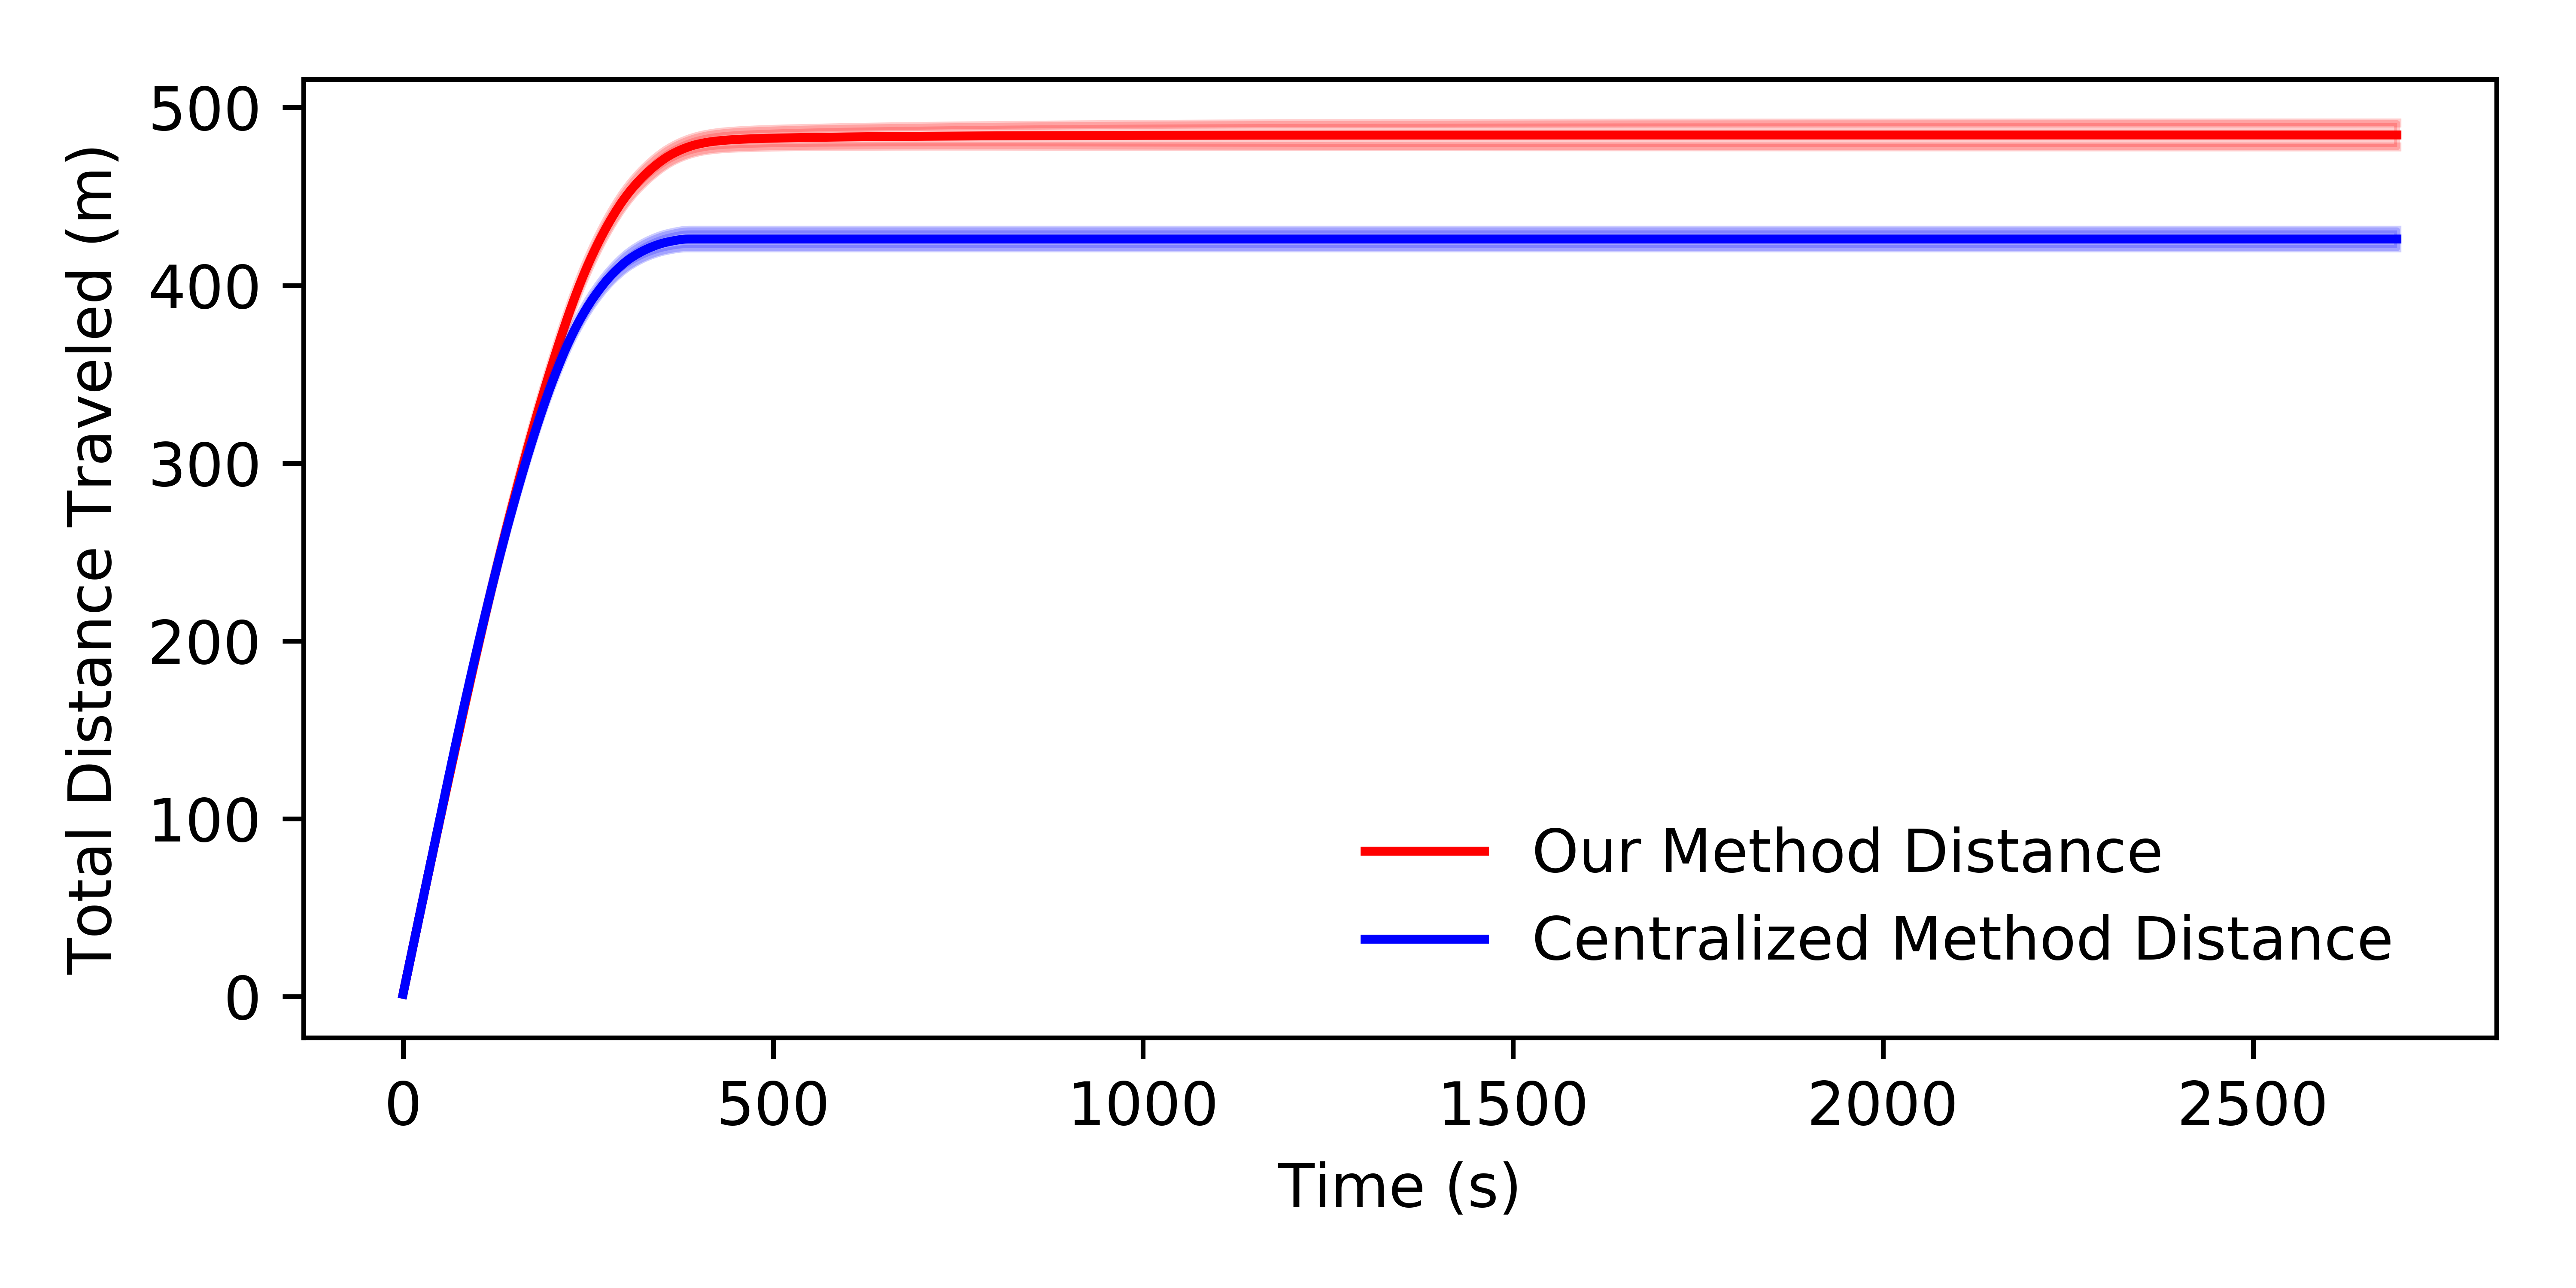
\includegraphics[trim=10pt 10pt 10pt 5pt, clip,width=0.48\textwidth]{IEEEtran/comparison/comparison_tro_dis.png}\\
\includegraphics[trim=10pt 10pt 10pt 5pt, clip,width=0.48\textwidth]{IEEEtran/comparison/comparison_tro.png}
\caption{Performance comparison between our method (red line) and centralized method (blue line). Each solid line in the plot is the average result from 40,000 simulations of 400 agents, and the colored shade areas show the confidence interval for convergence and total distance traveled over time at a confidence level of 2$\sigma$ (two standard deviations above or below the average).}
\label{fig:1222}
\end{figure}

\subsection{Experiments}

\begin{figure*}[t]
\centering
\includegraphics[width=1.0\textwidth]{variance/all_v.jpg}
\caption{Illustration of hardware used in experiments. \textbf{(\textit{1})} Key components of the \textit{Coachbot V2.0} swarm system: (1 \textit{Left}) Robot used in the experiments. The robot is in a cylinder shape with a height of 0.12m and a radius of 0.05m.  Key components are: ($a$) Localization system based on the HTC Vive, ($b$) Raspberry PI b+ computer, ($c$) electronics mother board, ($d$) rechargeable battery. (1 \textit{Right}) Robot arena used in experiments: ($e$) overhead camera (only used for recording videos), ($f$) overhead HTC Vive base station, ($g$) swarm of 100 robots. \textbf{(\textit{2})} Illustration of the \textit{Coachbot V2.0} swarm communication network. The green link is an ethernet connection between the base station and the Wi-Fi router.  The blue links are TCP/IP connections, and the black links are layer 2 broadcasting connections. \textbf{(\textit{3})} The swarm of 100 robots. \textbf{(\textit{4})} The robots charging by connecting to two metal strips attached to the wall. }
\label{fig:robot}
\end{figure*}



To validate the correctness and efficiency of our algorithm beyond simulation, we performed several physical experiments using the \textit{Coachbot V2.0} swarm system, a custom-made swarm of 100 differential-drive wheeled robots shown in Fig. \ref{fig:robot}.  

\subsubsection{Hardware}
\label{hardware}

There are two key components in the swarm's hardware design: the robot itself, and the base station used to manage and operate the swarm.

The design of \textit{Coachbot V2.0} consists of four key components: a main computer, localization module, power module, and locomotion module. The main computer is a Raspberry Pi 3b+ with a 1.4GHz 64-bit quad-core CPU, 1GB RAM, and dual-band 802.11ac wireless LAN (2.4GHz and 5GHz). The localization module, shown in Fig.\ref{fig:robot}, is a custom PCB consisting of two TS3633-CM1 sensors and an Atmel attiny87 microprocessor.  The two sensors receive infrared signals from the ceiling mounted \textit{HTC vive} lighthouse which emits a time-varying infrared pattern, allowing the sensors to determine their position.  The microprocessor calculates the positions of the two TS3633-CM1 sensors at an update rate of 30Hz, and sends the sensors' positions to the Raspberry Pi via the UART.  With this information, the main board can calculate the robot's orientation and position accurate up to $15^{\circ}$ and $0.04m$. The robot is powered by a 2.5Ah lithium-ion rechargeable battery, which is used to power the entire robot.  Additionally, a Bluetooth low energy module can disconnect the battery power from the rest of the robot.  This allows a user to send a Bluetooth command to put robots into a low-energy sleep mode as well as wake robots up from this sleep mode. With a fully charged battery robots can operate for approximately four hours, or sleep for three months. The robot drives across a flat surface using two wheels driven by DC motors.  An H-bridge controls the speed and direction of each motor independently, allowing for differential drive. Each robot has a height of 0.12m and a radius of 0.05m. 

A computer workstation manages all robots in the swarm at once, allowing a single person to easily operate the entire swarm without any direct interaction. However, the workstation does not control robots during experiments. The workstation can communicate with all robots using Wi-Fi, and can power the robots on and off using Bluetooth. Custom-made software on the workstation uses these capabilities to monitor the status of all robots, update the code executed on the swarm, start/stop the robots' program, turn them on/off, and collect the data from experiments.


\subsubsection{Software}
Software running in a modified version of raspbian operating system is running on board each robot's Raspberry Pi, controlling the robot's basic behaviors, robot-to-robot communication, and interaction with the base station. 

There are two separate communication channels in the system: a star network between base station and robots, and a mesh network among the robots. These two communication channels serve two separate tasks, see Fig. \ref{fig:robot} (\textit{2}).  Both channels make use of the Wi-Fi capabilities of the on-board Raspberry Pi. The star network is mainly used for transferring files between the base station and robots, i.e. uploading the user programs to the robots, while the other channel will support robot-to-robot communication used for the user programs.  The star network is implemented by connecting the robots to the base station's Wi-Fi router.  Communication along this channel uses standard TCP/IP protocol to ensure the reliable transfer of data and files.  For the robot-to-robot channel, communication uses layer 2 broadcasting, i.e. MAC address based broadcasting.  This allows robots to communicate with other robots directly, without use of the base station router.  By embedding the robot's position in the data packet, the robots' communication range in experiments can be artificially limited to a desired value by actively discarding messages which originate outside the desired communication range. In this papers experiments, the robots' communication range is limited to 0.4m. 


A custom coordination system makes use of the communication on the star network to operate and manage the swarm in a easy, scalable way \cite{swarmish, kilobot}. This system has three software components: a FTP server, a monitor module, and a broadcaster module. The FTP server is used to update the code running on the robots.  It can push new software to all robots at once.  The monitor module is used to monitor the status of all robots, which is transmitted from each robot to the base station.  It monitors information such as battery voltage, firmware version, etc. and displays it to the operator.  The broadcaster module is used to send commands to the swarm which help in its operation, such as starting and stopping execution of the user code, turning the robots on/off, and moving robots to a charging station.  The broadcaster module makes use of both Wi-Fi and Bluetooth communication. 

\subsubsection{Dealing with real-world non-idealities}
\label{experi}
In reality, some assumptions proposed in section \ref{assumptions} are difficult to be guaranteed in real robot hardware. To compensate the real-world non-idealities such as communication errors, imperfect robot motion, etc, we here relax the assumptions about proposed in section \ref{assumptions} as follows:

\begin{enumerate}[label=(\alph*), leftmargin=*]
   \item  For any agent, the frequency of its clock is bounded, specifically: $\exists f_{clock}^{max}, f_{clock}^{min}$ s.t. for any agent $a_i$, we have $f_{clock}^{min}\leq f_{clock}^i\leq f_{clock}^{max}$.

   \item  Note that for each agent $a_i$, its communication rate $f_{comm}^i$ is defined according to its on-board clock, i.e. the clock that is with frequency $f_{clock}^i$. As a result, even though each agent is programmed to broadcast at the same frequency $f_{comm}$ \textit{(alg. \ref{com module} Line 4)}, from a global observer's perspective, their communication rate could be still different due to the difference on clock's frequency $f_{clock}^i$. 

\item   The inter-agent communication packet loss rate is small enough such that: for each robot, if it sends the same message \textbf{\textit{m}} times in a row, it is guaranteed that this message can be received by all its neighbors in communication range.
 \item For any agent $a_i$, the speed $v_m^i$ at which it moves on a grid edge is bounded, namely: $\exists v_{max}, v_{min}$ s.t. for any agent $a_i$, we have $v_{min}\leq v_m^i\leq v_{max}$.
\end{enumerate}

First, note that as shown in section \ref{safety}, the proof of theorem \ref{collision free}, \ref{collision free2} does not rely on any assumption about robot's physical speed, in the other words, only the relaxation of assumption (a), (b), (c) will effect the correctness of theorem \ref{collision free}, \ref{collision free2}. To preserve the correctness of theorem \ref{collision free}, \ref{collision free2}, in practice, we extend $\Delta t$ to make the robot to act more conservatively, so as to compensate the difference on robots' clock frequency and packet loss. To be specific, we extend $\Delta t$ such that:

\begin{center}$\Delta t \geq \frac{2m}{f_{comm}}\frac{f_{clock}^{max}}{f_{clock}^{min}}$. \end{center}


One can observe that there are two terms on right hand side, the first term $\frac{2m}{f_{comm}^{min}}$ is for accommodating the communication loss, and the second term $\frac{f_{clock}^{max}}{f_{clock}^{min}}$ is for compensating the difference on robots' clock frequency. The reason for having the second term is that: when one agent executes \textit{alg. \ref{alg:main} Line 30} and \textit{alg. \ref{com module} Line 4}, it will use the on board clock to do the calculation, and different clock frequency will yield different results. Therefore, we add the second term to guarantee that: for the robot that is with the fastest clock, it will wait long enough to accommodate the one with the slowest clock. 

So far, we showed that the correctness of theorem \ref{collision free}, \ref{collision free2} can be preserved when the assumptions proposed in section \ref{assumptions} are relaxed. To guarantee the collision avoidance in practice, the next step is to come up with a strategy to accommodate the difference on robot's physical speeds, that is: when two agent $a_i, a_j$ move on two adjacent edges at the same time, let $v_m^i, v_m^j$ be the these two agents' speeds, if $v_{min}\leq v_m^i, v_m^j\leq v_{max}$, then no collision happens. Our strategy is stretching the grid length $l$ to give robots some ``buffered space" to compensate the difference on their speeds. Specifically, we want the $l$ large enough such that:
\begin{itemize}

    \item When two robots move on two orthogonal adjacent edges, no collision happens, that is: 
    
    \centering$\min_{t\leq \frac{l}{v_{max}}}\sqrt{(l-v_{max}t)^2 + (v_{min}t)^2} \geq 2r$,


\item \raggedright When two robots move on two collinear adjacent edges, no collision happens, that is: 

\centering$\min_{t\leq \frac{l}{v_{max}}}(l-v_{max}t + v_{min}t) \geq 2r$.

\end{itemize}

Solving those two inequalities above, we have:

\begin{center}{ $l\geq 2\frac{\sqrt{v_{max}^2 + v_{min}^2}}{v_{min}}r$.}\end{center} 


Additionally, in the algorithm, we have the assumption that the robot can move in any direction directly, which does not hold for the \textit{Coachbot V2.0}, as \textit{Coachbot V2.0} is a differential driven robots. When a \textit{Coachbot V2.0} moves from one waypoint $wp_{a}$ to another waypoint $wp_{b}$, it will first spin at waypoint $wp_{a}$ to adjust its orientation to be parallel with the grid edge connecting $wp_{a}$ and $wp_{b}$, before moving to $wp_{b}$. Note that for each step, the robot may change its orientation by $0$ \textit{rads} or $\frac{\pi}{2}$ \textit{rads} (because a differential driven robot can move both forwards and backwards, hence it does not need to adjust its orientation by more than $\pi$ \textit{rads}), to compensate this difference on the adjustments of the robot's heading, we introduce another type of  ``buffered space" to grid length, that is to say, assume the robot's minimal spin speed is $\omega^*$, we enforce the grid length $l$ to be:

\begin{center}{ $l\geq 2\frac{\sqrt{v_{max}^2 + v_{min}^2}}{v_{min}}r + v_{max}\frac{\pi}{2\omega^*}$.}\end{center} 




\subsubsection{Results}

In these physical experiments, we demonstrate that our algorithm can be easily implemented on a relatively large scale physical swarm, and it can provide reliable performance.  Additionally it is robust to real-world noise in both communication, sensing, and motion. In this experiment, 100 robots start randomly dispersed and form the letters ``N", ``U" in sequence.  With the help of hop-count information, robots can detect when the first letter is completed and then switch to form the second shape, an ``U".  Images from one of these experiments using our algorithm is shown in Fig. \ref{fig:frames1}.
We also compared the real-world performance between our algorithm and the centralized approach. A shape was formed 15 times with both approaches, and we compared the average convergence rate and average total distance traveled for both approaches. In all these 30 experiments,  the shape formation successfully completed. The results from this comparison experiment are shown in Fig. \ref{fig:experi}.


\begin{figure}[h!]
\centering
\includegraphics[trim=10pt 10pt 10pt 5pt, clip,width=0.48\textwidth]{IEEEtran/comparison/experi/comparison_experi_con.png}\\
\includegraphics[trim=10pt 10pt 10pt 5pt, clip,width=0.48\textwidth]{IEEEtran/comparison/experi/comparison_experi_dis.png}
\caption{Illustration of average performance comparison between our method (red line) and the centralized method (blue line). Each solid line is the average result from 15 physical experiments of 100 robots, and the colored shade areas show the confidence interval for convergence and total distance traveled over time at a confidence level of 2$\sigma$ (two standard deviations above or below the average)}
\label{fig:experi}
\end{figure}

In these plots, we can observe that the our method gets a short-term win
at the beginning compared to the centralized method, which is consistent with the simulation result. On the other hand, one observation here is that in the simulation plots (Fig. \ref{fig:1222}), both the convergence and the distance traveled monotonically increase over time, whereas in Fig. \ref{fig:frames1}, during the first 20 seconds, the convergence plot is sharply fluctuated. This is because in simulation the agents are tasked to form a set of random shapes from a random initialization of positions whereas in all physical experiments the robots are tasked to form the same shape, letter ``N", which will introduce the bias to the final result. Besides that, in the reality, there will be noise in robot's motion, communication, and sensing, which can not be captured by the simulation very well, and the number of trials are not large enough to eliminate the noise's effect on the convergence rate, as a result, the convergence plot for physical experiment is not monotonically increasing over time. 




To be implemented in the real world, our methods requires the robots to be able to measure its own position and orientation in a global coordination system. Moreover, since the robot moves in a grid world, there will be a lot of twists and brakings, which makes the robot's motion not very efficient. 

\section{Conclusion}

In this paper, we introduced a fully distributed shape formation algorithm which enables a swarm of robots to move and form a user-specified shape quickly and without collision. With this algorithm, agents take an array of goal points as input, then use the local information to distribute the goals among the swarm and schedule the collision-free paths concurrently. To demonstrate the correctness and performance of our algorithm, we executed our algorithm on a swarm of up to 1024 simulated robots, and 100 real robots.  The result of these experiments shows that this algorithm can reliably converge to all robots forming the desired shape. Additionally, the large numbers of simulation trials as well the real robot experiments showed that it can do so with only a small difference, around $25\%$ to be specific, in travel distances when compared to an optimal centralized approach. 


\printbibliography
% If you have an EPS/PDF photo (graphicx package needed) extra braces are
% needed around the contents of the optional argument to biography to prevent
% the LaTeX parser from getting confused when it sees the complicated
% \includegraphics command within an optional argument. (You could create
% your own custom macro containing the \includegraphics command to make things
% simpler here.)
%\begin{IEEEbiography}[{\includegraphics[width=1in,height=1.25in,clip,keepaspectratio]{mshell}}]{Michael Shell}
% or if you just want to reserve a space for a photo:
\begin{IEEEbiography}[{\includegraphics[width=1in,height=1.25in,clip,keepaspectratio]{hanlin.png}}]{Hanlin Wang}
is currently a Ph.D candidate in the department of computer science at Northwestern University.
He received the B.S. degree in mechanical engineering from Shanghai Jiao Tong University, Shanghai, China, in 2015. His research interests include multi-robot systems, distributed computation systems, and robotics.
\end{IEEEbiography}
\begin{IEEEbiography}[{\includegraphics[width=1in,height=1.25in,clip,keepaspectratio]{mike.jpg}}]{Michael Rubenstein}
is currently a assistant professor 
working on swarm robotics and control in the department of computer science as well as department of mechanical engineering at Northwestern University.
He received his Ph.D. from the University of Southern
California. His research interests include robot swarms and multi-robot systems.
\end{IEEEbiography}
\begin{comment}
% if you will not have a photo at all:
\begin{IEEEbiographynophoto}{John Doe}
Biography text here.
\end{IEEEbiographynophoto}

% insert where needed to balance the two columns on the last page with
% biographies
%\newpage

\begin{IEEEbiographynophoto}{Jane Doe}
Biography text here.
\end{IEEEbiographynophoto}
\end{comment}
% You can push biographies down or up by placing
% a \vfill before or after them. The appropriate
% use of \vfill depends on what kind of text is
% on the last page and whether or not the columns
% are being equalized.

%\vfill

% Can be used to pull up biographies so that the bottom of the last one
% is flush with the other column.
%\enlargethispage{-5in}



% that's all folks
\end{document}


